\chapter{Article : Three-Dimensional Multilayer Ice Accretion Using a Level-Set Method}\label{sec:lsArticle}

\textit
{
This chapter presents a continuous level-set framework for simulating 3D ice accretion within a quasi-steady, multilayer approach. In contrast to traditional Lagrangian surface-node displacement methods, which may suffer from mesh distortion and topological limitations, the proposed method relies on an implicit interface-capturing formulation that naturally represents complex geometric features and topological changes. The continuous level-set equation is solved on adapted meshes using a conservative formulation combined with a semi-implicit Rosenbrock-Wanner time integration scheme. A local interface-reconstruction procedure is introduced to monitor and control the accreted ice volume without requiring full surface extraction. The zero level set is then extracted using an external library (\textup{\textsc{MMG}}) to generate a conformal surface mesh. To reduce numerical oscillations while preserving the overall ice shape and volume, a smoothing filter is applied to the extracted surface. The proposed methodology is assessed on representative icing configurations, including a manufactured test case and experimental cases from the first Ice Prediction Workshop (IPW1). The results demonstrate good agreement with reference and experimental data.
}

\par\vspace{0.5cm}

\noindent\textit{Submitted to Computers \& Fluids on 22 June 2026 (under review).}

\section{Introduction}
\label{sec:introduction}
Ice accretion on aircraft components remains a critical challenge for the aerospace industry. The resulting geometrical changes on lifting surfaces can significantly alter the aerodynamic characteristics of the aircraft. In particular, ice accretion leads to a reduction in aerodynamic efficiency, characterized by a decrease in the maximum lift coefficient ($C_{L,\max}$) and an increase in drag \cite{CAO2018353}. In more severe situations, however, ice accumulation can compromise aircraft controllability and potentially endanger flight safety.

To better understand and control these phenomena, numerical tools are increasingly employed. Advances in computational methods and high-performance computing (HPC) have significantly improved the capability of simulation frameworks to capture the complex multiphysics processes involved in ice accretion. As a result, numerical modeling has become an essential component of the aircraft design and certification process, enabling more reliable predictions of ice formation and its aerodynamic consequences \cite{broeren2011aerodynamic}.

Ice accretion is an unsteady and intricate multiphysics phenomenon involving the interaction of aerodynamic flow, droplet dynamics, thermodynamic exchanges, and geometric evolution. However, the characteristic time scales of ice growth are significantly larger than those of the underlying physical processes (e.g. flow fluctuations). As a result, the accretion process can be modeled using a quasi-steady framework in which the total icing exposure time is subdivided into \(N\) successive discrete steps \cite{KIND1998257}. At each step, the governing equations are solved assuming steady-state conditions, after which the geometry is updated. This procedure corresponds to the commonly adopted multilayer approach for ice accretion simulations. Figure~\ref{fig:icing_framework} illustrates a typical icing simulation workflow. The simulation begins with a clean geometry, which can either be meshed to generate a body-fitted computational grid or embedded within a pre-existing background mesh in the case of immersed boundary approaches \cite{pabloIcing}. A flow solver is first used to compute the airflow around the geometry, often using the Reynolds-Averaged Navier-Stokes equations (RANS). This is followed by droplet tracking to determine the distribution of liquid water on the wetted surfaces. Subsequently, thermodynamic exchanges are evaluated to estimate the local ice mass accretion rate. Finally, the geometry is advanced using a time-accurate update algorithm to account for the newly formed ice shape. The resulting modified surface is then used to update the surrounding volume mesh accordingly.

\begin{figure}[htbp] 
    \centering
    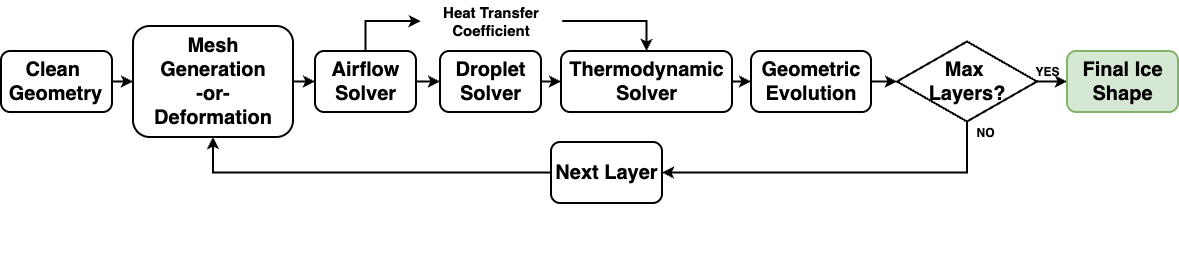
\includegraphics[width=1.0\textwidth]{FIGURES/LEVELSET_ARTICLE/icingFramework.png}
\caption{Schematic of the multilayer ice accretion framework.}
    \label{fig:icing_framework}
\end{figure}

Although all these steps remain active areas of research, the present work focuses on the last stage of the framework: the geometric evolution required to represent the accreted ice shape. This aspect has received considerable attention in recent years due to the inherent topological challenges associated with ice growth. Early approaches relied on Lagrangian displacement of surface nodes along their local normals \cite{thompsonDeformation}, accompanied by a volume propagation of the deformation. While these methods are computationally efficient and relatively straightforward to implement, they encounter significant difficulties when complex ice shapes develop, particularly in the presence of concave and convex regions where mesh entanglement can occur. Such methods do not inherently resolve these topological issues. Although heuristic strategies can sometimes mitigate these problems in 2D configurations by removing problematic nodes or locally adjusting the geometry, extending these techniques to 3D becomes considerably more challenging due to the complexity of stitching and merging surface regions \cite{glimm2000}.  More recently, surface-wrapping techniques have been used to circumvent some of these topological limitations in complex ice-accretion simulations \cite{Ozcer_2019}.

An increasingly popular alternative is to represent the evolving ice geometry implicitly using interface-capturing methods such as level-set formulations \cite{OSHER2004}. Level-set methods have been widely used to model moving-interface problems across a broad range of applications, including multiphase flows \cite{twoPhaseFlow, multiphaseFlowLS}, shape optimization \cite{ALLAIRE20211}, and forest-fire propagation \cite{MALLET20091089}, to name a few. In this approach, the interface is described by a level-set function $\phi$, whose evolution is governed by an advection equation driven by a velocity field. In the context of aircraft icing, an early use of the level-set method was reported by \cite{HeloiseBeaugendre}, where it was employed to track ice-shedding trajectories rather than to model the accretion process itself. Subsequent developments extended the use of level-set methods to ice accretion. One of the earliest formulations in this direction was proposed by \cite{PENA2016278}, and later extended by \cite{bourgault-coteMultilayerAirfoilIce2019}, who modified the icing velocity field while still relying on explicit Lagrangian tracking of surface nodes to extract the ice shape. These approaches were applied on RANS meshes, where strict mesh-resolution requirements and time-step constraints can limit the effectiveness of level-set evolution. More recently, \cite{alessandroLevelSet} introduced a discrete formulation of the level-set method based on a Lagrangian prediction of the ice shape. While this approach proved effective, conservation of the accreted ice mass remained dependent on the quality of the underlying Lagrangian displacement, which can still suffer from mesh distortion and entanglement.

The present work addresses this gap in the literature by adopting a framework for solving the level-set equations on adapted meshes, thereby alleviating constraints imposed by the computational mesh. In particular, the level-set formulation is solved in its continuous form within a multilayer accretion framework. To the best of the authors' knowledge, this work represents one of the first extensions of a partial-differential-equation-based level-set formulation to 3D multilayer ice accretion. In addition, a robust and efficient time integration strategy, namely the Rosenbrock-Wanner scheme, is employed to accelerate the solution process while maintaining numerical stability. The proposed methodology enables consistent monitoring and control of the accreted ice volume through a local interface-reconstruction procedure, while simultaneously generating a conformal geometry suitable for subsequent simulation layers. Overall, the approach provides a robust, consistent, and scalable framework for 3D ice accretion simulations.

The remainder of this paper is organized as follows. Section~\ref{sec:framework} presents the CHAMPS icing framework and the overall simulation strategy. Section~\ref{sec:level_set_formulation} introduces the level-set formulation, including the governing equations, velocity models, and time integration approach. Section~\ref{sec:geometry_processing} describes the geometry extraction and smoothing procedures used to obtain conformal ice shapes. The proposed methodology is then assessed and discussed in Section~\ref{sec:results} through representative test cases. Finally, conclusions and perspectives are provided in Section~\ref{sec:conclusionsLS}.

\section{CHAMPS Icing Framework}
\label{sec:framework}

The present work is implemented within \textsc{CHAMPS} \cite{champsArticle}, an in-house 3D unstructured cell-centered finite-volume solver developed at Polytechnique Montr\'eal. Under the quasi-steady icing assumption, the total icing exposure time is discretized into \(N\) discrete layers (Fig.~\ref{fig:icing_framework}). For each layer, the flow field is computed using a RANS solver with Roe-based convective fluxes, a weighted least-squares gradient reconstruction, and a Venkatakrishnan limiter.

The aerodynamic solution is followed by Lagrangian droplet tracking \cite{ZAYNI2026112019} in order to determine the water catch distribution $\beta$ on the wetted surfaces. Water droplets are released from an upstream seeding plane located in an unperturbed region of the flow ($u_{\mathrm{local}}/u_{\infty} \approx 0.9$) and tracked until impact with the surface. Rather than assuming a single droplet diameter, a polydispersed droplet cloud is considered to better reproduce the experimental conditions. Multiple droplet size bins are simulated successively and then combined through a weighted procedure to obtain the final impingement distribution $\beta$.

Ice accretion is then computed using an iterative Messinger model \cite{Zhu_2014} that resolves the thermodynamic exchanges at the surface. This model relies on mass and energy balances applied locally at each surface cell and embedded within an iterative loop to determine the incoming and outgoing water fluxes. The resulting solution yields the local ice mass accretion rate, $\dot{m}_{\text{ice}}$, which drives the geometric evolution of the ice layer.

The geometric update can be performed either through a Lagrangian surface displacement approach \cite{thompsonDeformation}, in which the computed ice accretion rate $\dot{m}_{\text{ice}}$ is used to determine the displacement velocity of surface nodes, or through the level-set method \cite{OSHER2004} considered in the present work. In the latter case, the ice interface is tracked implicitly within an unsteady Eulerian framework and subsequently extracted to obtain a conformal surface mesh representing the updated ice geometry.

Finally, to complete the accretion layer, a remeshing stage is performed in order to generate a new volume grid for the subsequent icing step. In 2D, this remeshing stage relies on an in-house hyperbolic mesh generator \cite{bourgault2019ice}. For 3D simulations, the volume mesh is generated using \textsc{Pointwise} scripts \cite{fidelity_pointwise_2025}.


\section{Level-Set Ice Accretion Formulation}
\label{sec:level_set_formulation}

\subsection{Level-Set Governing Equations and Initialization}
\label{subsec:levelset_governing}

The level-set method, introduced by \cite{OSHER198812}, provides a robust framework for tracking moving interfaces through a Hamilton--Jacobi formulation. An illustration of the level-set field is given in Fig.~\ref{fig:IceAirInterface}. Its primary objective is to represent evolving boundaries implicitly within an unsteady Eulerian framework. Following \cite{FROLKOVIC2015214}, the level-set equation can be written in conservative form for the signed distance function $\phi$ (Eq.~\ref{eq:levelSet}):

\begin{equation}
\begin{gathered}
\frac{\partial \phi}{\partial t} 
+ \nabla \cdot (\phi \boldsymbol{V})  
- \phi \nabla \cdot \boldsymbol{V} = 0, \\[6pt]
\phi =
\begin{cases}
< 0 & \text{in the solid (ice) region}, \\
= 0 & \text{at the interface}, \\
> 0 & \text{in the fluid (air) domain}.
\end{cases}
\end{gathered}
\label{eq:levelSet}
\end{equation}

\begin{figure}[htbp] 
    \centering
    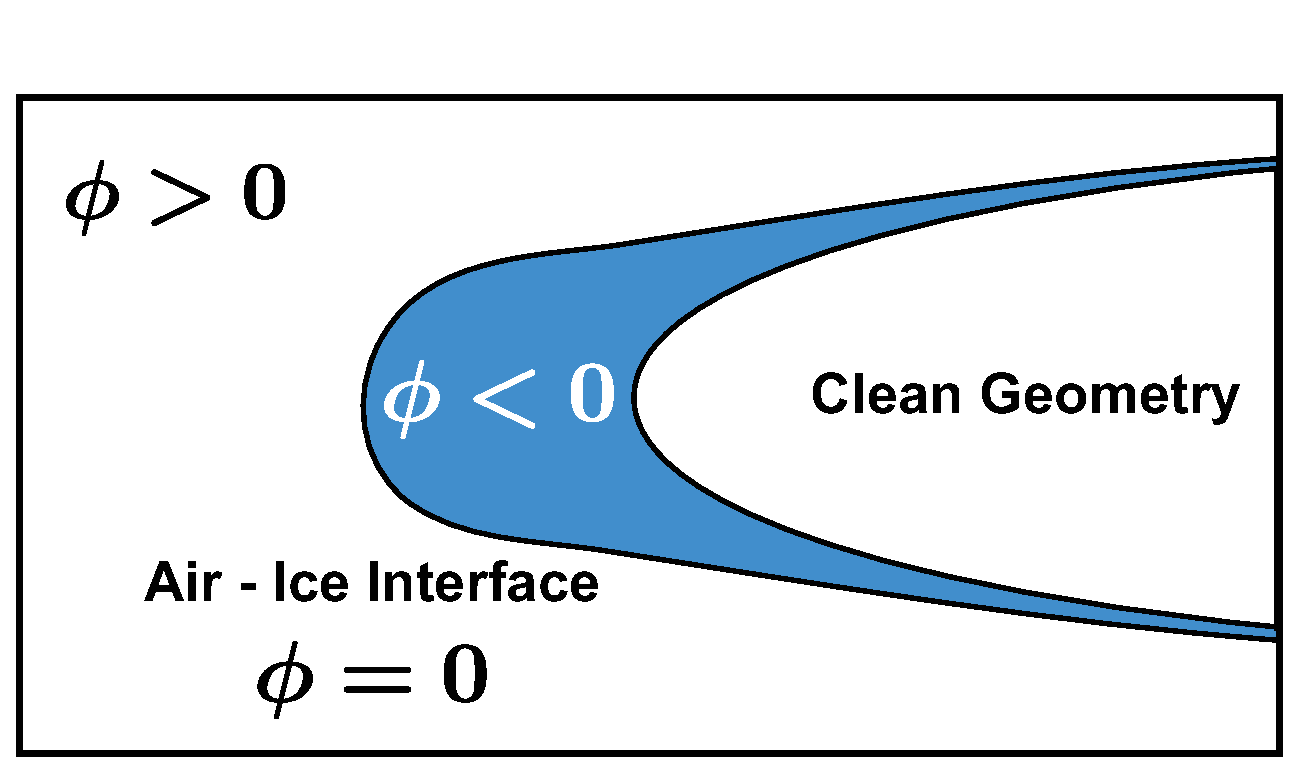
\includegraphics[trim={0cm 0cm 0cm 0cm},clip,width=0.5\textwidth]{FIGURES/LEVELSET_ARTICLE/ICE_AIR_INTERFACE.eps}
    \caption{Representation of the level-set function $\phi$. The ice region is defined by $\phi < 0$ (blue), while the surrounding air corresponds to $\phi > 0$. The interface is implicitly represented by the zero level set $\phi = 0$.}
    \label{fig:IceAirInterface}
\end{figure}

In Eq.~\ref{eq:levelSet}, $t$ denotes the physical time and $\boldsymbol{V}$ represents the interface velocity field. The equation is solved in an unsteady manner. A linear extrapolation boundary condition is applied at all domain boundaries along the level-set unit normal direction, defined as $\boldsymbol{n}_{\phi} = \frac{\nabla \phi}{\|\nabla \phi\|}$. The extrapolated value is obtained using the distance vector between the ghost-cell center and the adjacent interior cell center.

The initial level-set field is defined as a wall-distance field. A natural approach to compute this field consists in solving the steady form of the level-set equation \cite{tuckerEikonal}, commonly referred to as the Eikonal equation (Eq.~\ref{eq:eikonal}). This equation is solved using a pseudo-time \(\tau\) scheme, which vanishes upon convergence. 

\begin{equation}
\frac{\partial \phi}{\partial \tau} + \boldsymbol{n}_{\phi} \cdot \nabla \phi = 1
\label{eq:eikonal}
\end{equation}

\noindent Owing to its unit source term, the Eikonal equation enforces a unit norm of the level-set gradient, thereby ensuring the signed-distance property. In this formulation, the extrapolation boundary condition is replaced by a Dirichlet condition imposed at the wall, \(\phi_{\text{wall}} = 0\). Figure~\ref{fig:EikonalSolution} shows the Eikonal contours around a NACA 23012 airfoil, which represent the resulting wall-distance field.



\begin{figure}[htbp] 
    \centering
    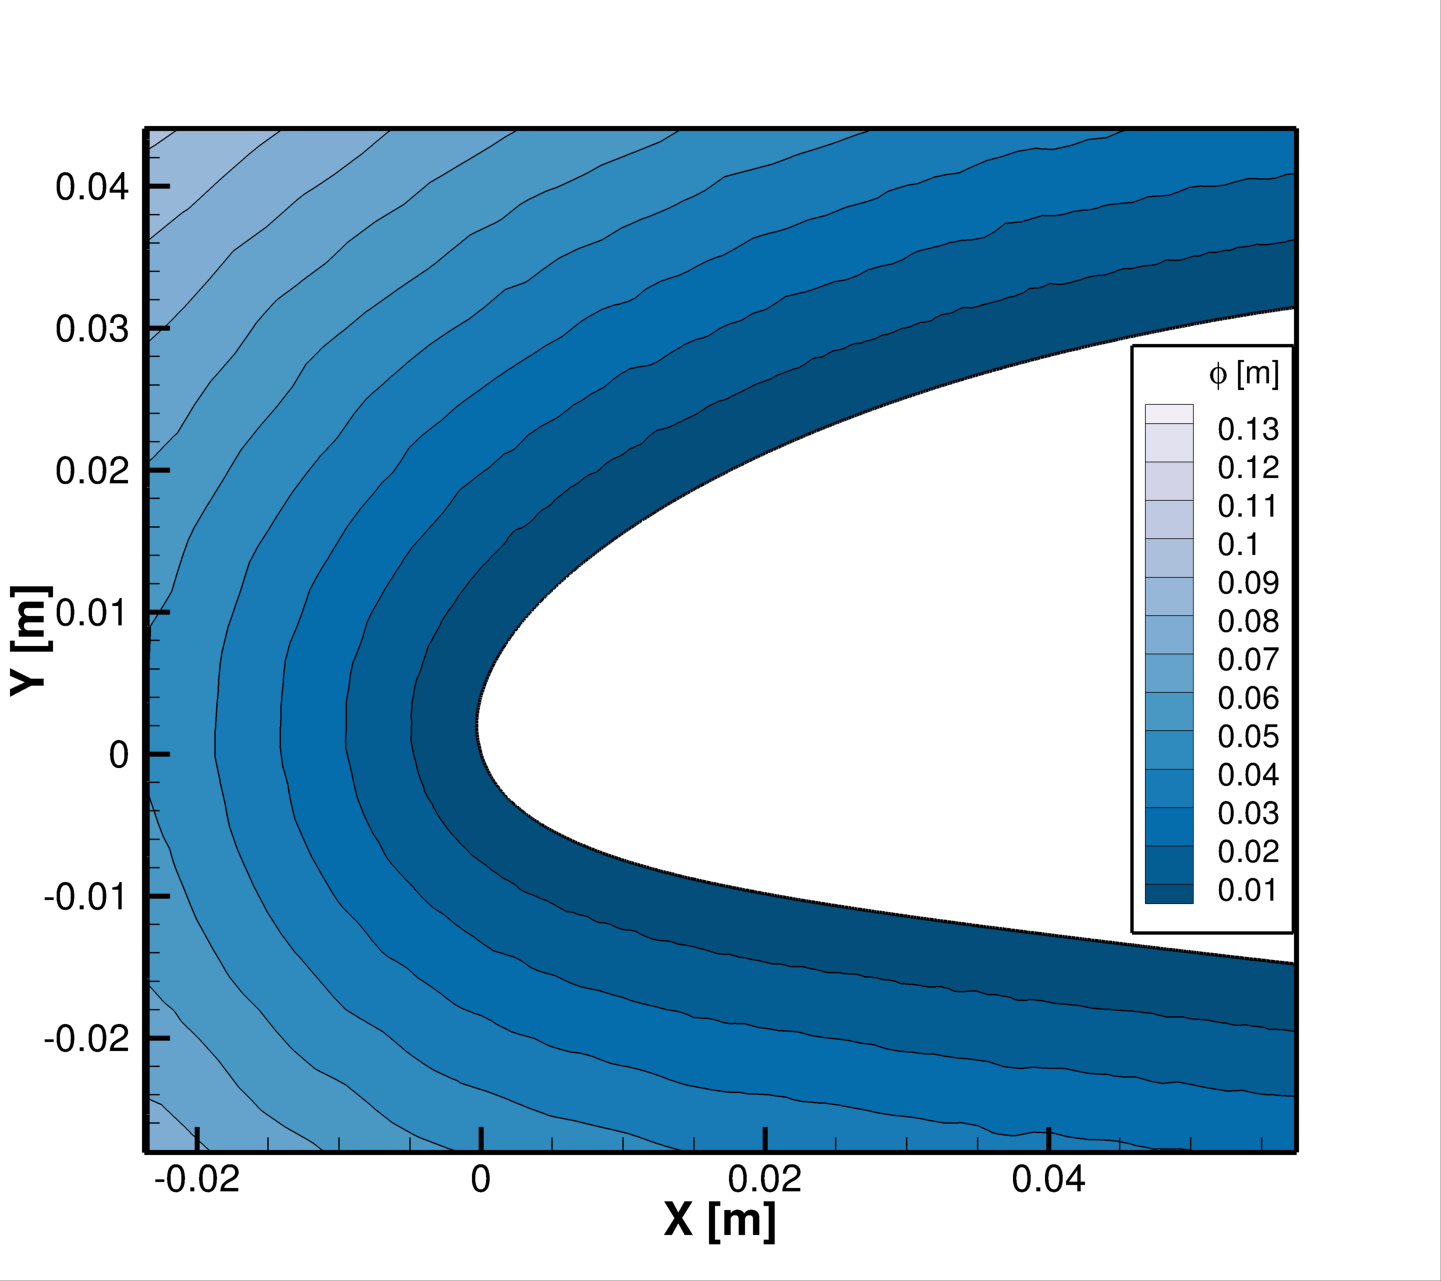
\includegraphics[trim={0cm 1cm 3cm 3cm}, clip, width=0.5\textwidth]{FIGURES/LEVELSET_ARTICLE/EIKONAL.png}
    \caption{Contours of the level-set function $\phi$ obtained from the Eikonal equation, representing the wall-distance field.}
    \label{fig:EikonalSolution}
\end{figure}

\subsection{Level-Set Advection: Velocity Formulation, Surface-Quantity Propagation, and Time Integration}
\label{subsec:icing_velocity}

The velocity field governing interface motion must be related to the ice accretion variables. Three main approaches have been proposed in the literature and are summarized in Table~\ref{tab:velocityFormulation}. The work of \cite{PENA2016278} first introduced a surface-based icing-velocity formulation (Eq.~\ref{eq:IcingVelocityDorian}), in which the interface velocity depends exclusively on surface quantities. In this formulation, the three velocity components computed at the surface must be propagated throughout the level-set computational domain. In Eq.~\ref{eq:IcingVelocityDorian}, $\dot{m}_{ice}$ denotes the ice mass accretion rate and $\rho_{ice}$ the ice density.

\begin{equation}
\boldsymbol{V} = \frac{\dot{m}_{ice}}{\rho_{ice} A_{wall}} \boldsymbol{n}_{wall}
\label{eq:IcingVelocityDorian}
\end{equation}

The approach proposed by \cite{bourgault-coteMultilayerAirfoilIce2019} later pointed out that this formulation introduces an implicit dependency on the local surface area, which should evolve with the deformation of the interface. A flux-based velocity formulation (Eq.~\ref{eq:fluxIcingVelocity}) was therefore proposed, in which the ice accretion rate is first propagated within the volume and then locally adjusted according to a characteristic area. This formulation is intended to improve local volume conservation.

\begin{equation}
\boldsymbol{V} = \frac{\dot{m}_{ice}}{\rho_{ice} \, \Delta A_{local}} \boldsymbol{n}_{\phi}
\label{eq:fluxIcingVelocity}
\end{equation}

\noindent where the projected local area $\Delta A_{local}$ is defined as

\begin{equation}
\Delta A_{local} = \sum_{facets} 
\left| \boldsymbol{n}_f \cdot \boldsymbol{n}_{\phi} \right| \Delta A_{facet}
\label{eq:cellCharacteristic}
\end{equation}

\noindent In Eq.~\ref{eq:cellCharacteristic}, $\boldsymbol{n}_f$ denotes the facet normal and $\Delta A_{facet}$ the corresponding facet area.

The formulation introduced by \cite{lavoieLevelSet} constitutes a further improvement over that of \cite{PENA2016278}. In this approach, the velocity magnitude remains constant and is propagated along the $\phi$-normals, while its direction is computed locally from the initial $\phi$-normals. This feature is particularly attractive in the present context, as it helps preserve the signed-distance property of the level-set field and thereby limits the need for re-initialization \cite{FROLKOVIC2015214}. For this reason, this formulation is adopted in the present work.

\begin{equation}
\begin{aligned}
\boldsymbol{V} &= \frac{h_{ice}}{\Delta t_{icing}} \boldsymbol{n}_{\phi}
= \frac{\dot{m}_{ice}}{\rho_{ice} A_{wall}} \boldsymbol{n}_{\phi}, \\
h_{ice} &= \frac{\Delta t_{icing} \, \dot{m}_{ice}}{\rho_{ice} \, A_{wall}}.
\end{aligned}
\label{eq:distanceIcingVelocity}
\end{equation}

\begin{table}[ht]
\centering
\caption{Icing Velocity Formulations}
\begin{tabular}{ccc}
\hline \hline
Icing Velocity & Norm & Direction \\ 
\hline
Pena et al. \cite{PENA2016278} & $\dot{m}_{ice} / (\rho_{ice} A_{wall})$ & $\boldsymbol{n}_{wall}$ \\ 
Bourgeault-Côté et al. \cite{bourgault2019ice} & $\dot{m}_{ice} / (\rho_{ice} \, \Delta A_{local})$ & $\boldsymbol{n}_{\phi}$ \\ 
Lavoie et al. \cite{lavoieLevelSet} & $h_{ice} / \Delta t_{icing}$ & $\boldsymbol{n}_{\phi}$ \\ 
\hline \hline
\end{tabular}
\label{tab:velocityFormulation}
\end{table}

Since the chosen interface velocity is defined from surface quantities, such as $\dot{m}_{ice}$ and $h_{ice}$, these must be extended into the volume. This is achieved by solving a convection equation \cite{bourgault2019ice} that propagates the variable along the $\phi$-normals:

\begin{equation}
\frac{\partial \varphi}{\partial \tau} + \nabla \cdot (\varphi \boldsymbol{n}_{\phi}) - \varphi \nabla \cdot \boldsymbol{n}_{\phi} = 0
\label{eq:propagation}
\end{equation}

Here, $\varphi$ denotes the propagated quantity. A Dirichlet boundary condition is imposed at the wall, while a zero-gradient Neumann condition is prescribed at the far field. An example of the resulting propagated field is shown in Fig.~\ref{fig:IceThicknessPropagated}. It should be noted that the Eikonal and propagation equations described above are not the only possible approaches for initializing the level-set field and extending surface information into the volume. In the present study, a geometric wall-distance method based on \cite{schneider2002geometric} was also tested. With this approach, the wall distance is computed in the volume, while the propagated quantity is assigned from the closest wall cell. Both approaches yielded similar results.

\begin{figure}[htbp] 
    \centering
    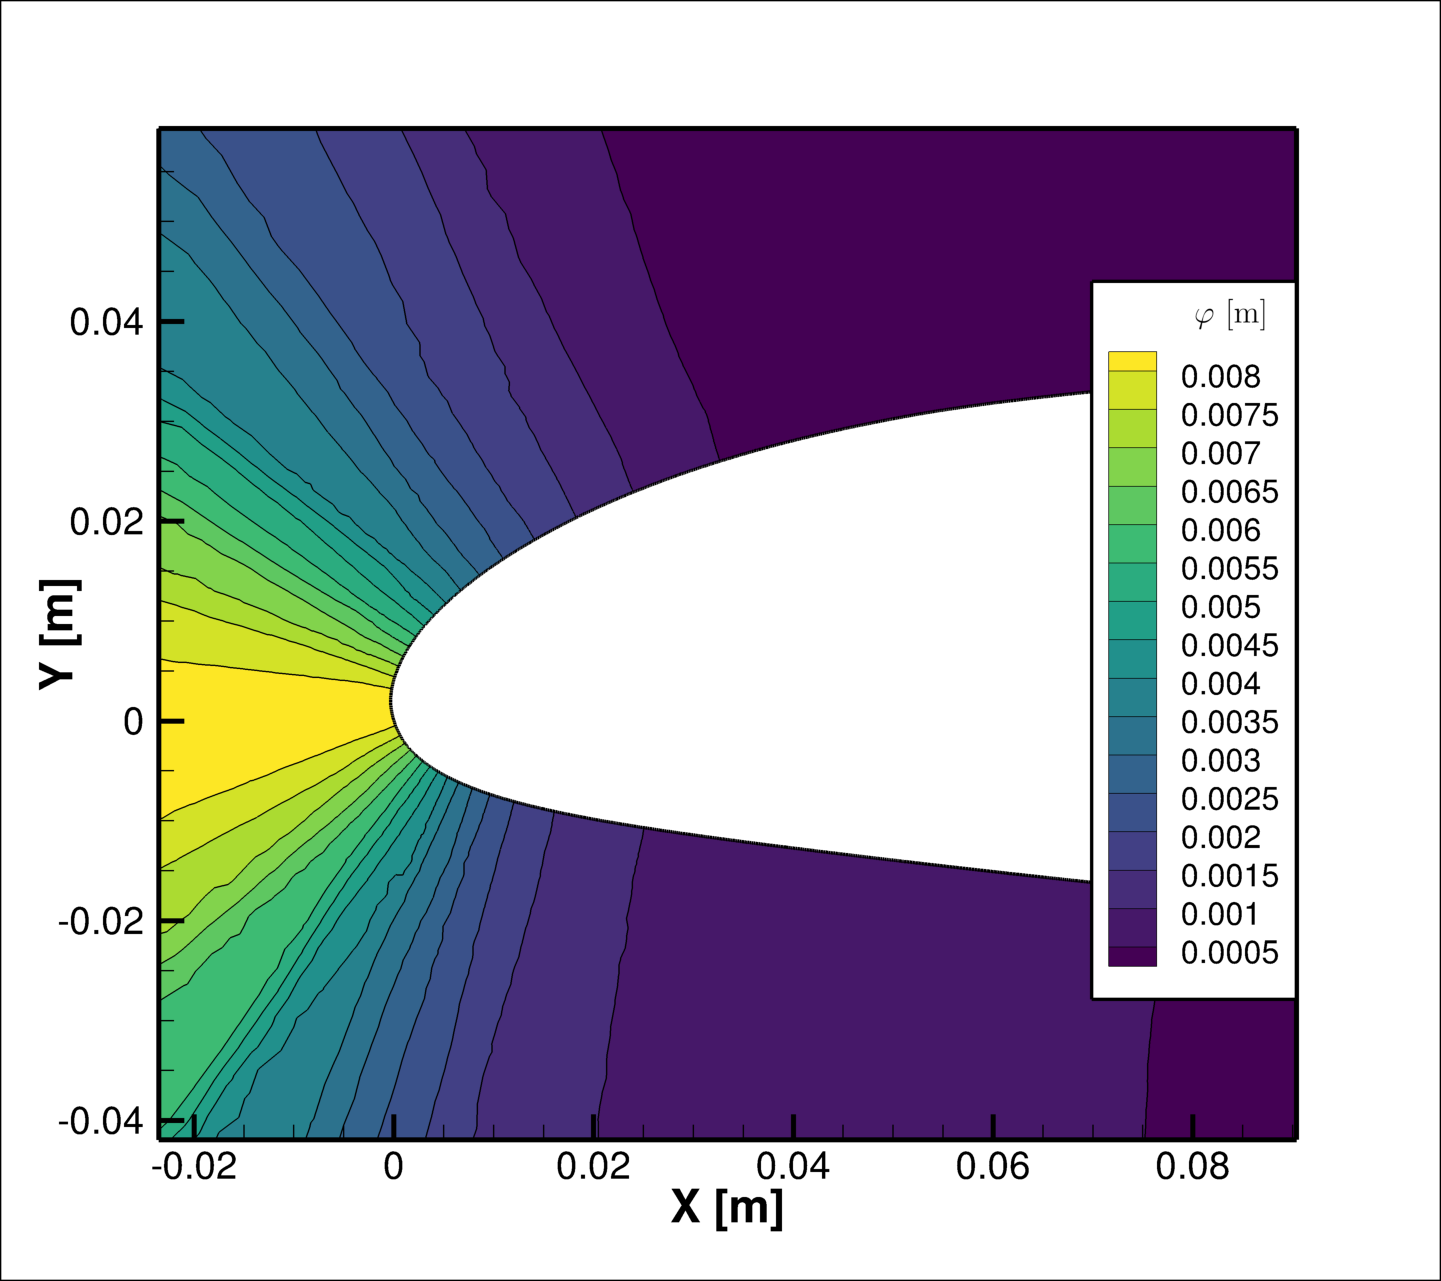
\includegraphics[trim={1cm 1cm 3cm 3cm}, clip, width=0.5\textwidth]{FIGURES/LEVELSET_ARTICLE/PROPAGATION.png}
    \caption{Contours of the propagated scalar field $\varphi$, here representing the ice thickness extended from the clean surface into the volume. The field is transported along the $\phi$-normal direction.}
    \label{fig:IceThicknessPropagated}
\end{figure}

% The choice of interface-velocity formulation is closely related to the time-integration strategy, since both influence the preservation of the signed-distance property, the robustness of the advection step, and the overall computational cost. When the interface velocity varies along the $\phi$-normals, the signed-distance property of the level-set function is no longer preserved during advection. As a result, the gradient of $\phi$ deviates from unity and the level-set field progressively departs from a signed-distance function. This degradation negatively impacts the conditioning of the numerical system and may compromise the accuracy of the solution \cite{OSHER2004}.

% To restore the signed-distance property, a re-initialization step is commonly introduced. This procedure is typically formulated as a modified Eikonal equation involving a Heaviside function $H(\phi)$, which prevents modifications of the solution in the vicinity of the interface:

% \begin{equation}
% \frac{\partial \phi}{\partial \tau} + H(\phi) \boldsymbol{n}_{\phi} \cdot \nabla \phi = H(\phi)
% \label{eq:reinitialization}
% \end{equation}

% Re-initialization must be applied carefully to avoid shifting the interface location \cite{bourgault2019ice}. Furthermore, no consensus exists regarding its optimal frequency. This operation is nevertheless essential in applications where the signed-distance property is required, such as the evaluation of geometric quantities (normals and curvature) or in coupled models including immersed boundary methods and turbulence models, where the distance to the interface directly influences source terms and boundary conditions.

% In ice accretion applications, the interface evolution generally remains smooth and is not characterized by large deformations. In addition, the present work focuses on a multilayer accretion strategy, in which the interface displacement at each step remains small and a significant portion of the geometry remains unchanged. These characteristics reduce the severity of signed-distance degradation. Furthermore, \cite{FROLKOVIC2015214} showed that when the interface velocity remains constant along the level-set normals, the signed-distance property can be preserved more effectively, thereby reducing, or even eliminating, the need for re-initialization. These considerations further support the use of the interface-velocity formulation proposed by \cite{lavoieLevelSet} in the present work.

Beyond the choice of interface-velocity formulation, the time-integration strategy also has a direct impact on robustness and computational efficiency. Most existing level-set-based icing approaches rely on explicit time integration schemes \cite{PENA2016278,lavoieLevelSet}, which impose restrictive stability constraints on the time step, or on dual time stepping methods \cite{bourgault-coteMultilayerAirfoilIce2019}, which require additional pseudo-time iterations and thereby increase computational cost.

In contrast, the present work employs a Rosenbrock--Wanner (ROW) semi-implicit time integration scheme \cite{hairer1996} recently introduced in CHAMPS and presented at the Cambridge Unsteady Flow Symposium (CUFS 2026) \cite{CUFS2026}. This approach improves stability and allows for larger time steps. In the present context, this feature is particularly advantageous since the multilayer ice accretion framework involves only small surface deformations at each accretion step. As a result, the signed-distance property of the level-set field is better preserved, which significantly reduces the need for re-initialization in the accretion cases considered here. The two-stage scheme is given in Eq.~\ref{eq:ROW2}:

\begin{equation}
\begin{gathered}
\phi^{n+1} = \phi^n + \sum^{s}_{j=1} m_j S_j \\[6pt]
\left(\frac{\boldsymbol{I}}{\gamma \Delta t}  + \boldsymbol{J}\right)^n S_i = -R\left(\phi^n + \sum^{i-1}_{j=1} a_{ij} S_j\right) \\[6pt]
\gamma = 1 - \frac{1}{\sqrt{2}} \\[6pt]
\boldsymbol{A} =
\begin{pmatrix}
0 & 0 \\
4 - 8\gamma & 0
\end{pmatrix},
\qquad
\boldsymbol{m}^{T} =
\begin{pmatrix}
\dfrac{1}{\gamma}\left(1 - \dfrac{1}{8\gamma}\right) \\[6pt]
\dfrac{1}{8\gamma^{2}}
\end{pmatrix}.
\end{gathered}
\label{eq:ROW2}
\end{equation}

\noindent where \(R(\phi)\) denotes the spatial residual associated with the semi-discrete level-set equation, \(\boldsymbol{J}=\partial R/\partial \phi\) is the corresponding Jacobian matrix, \(S_i\) are the stage increments. This formulation resembles a two-stage Runge--Kutta scheme, with the distinction that the Jacobian matrix appears on the left-hand side, leading to the solution of a linear system at each stage. In the present work, this system is solved using the Generalized Minimal Residual (GMRES) method \cite{GMRES}.%, and the Jacobian matrix was evaluated analytically.

\subsection{Ice Mass Computation and Local Interface Reconstruction}
\label{subsec:volume_reconstruction}

The global ice mass is evaluated at each time step by integrating the volume of the region where $\phi < 0$, allowing the simulation to terminate at the prescribed total ice mass. In the present work, variable ice density is not currently considered; therefore, the mass is assumed to be directly proportional to the accumulated volume. Cells are first classified according to the sign of $\phi$ at their nodes: cells located entirely within the ice region contribute fully to the volume, whereas intersected cells require a partial volume evaluation. In the latter case, a local interface reconstruction is performed only within the intersected cells, following the different intersection configurations illustrated in Fig.~\ref{fig:LocalExtraction}, thereby avoiding the cost of a full surface extraction. This local treatment is sufficient for volume estimation and remains inexpensive to evaluate at each time step. The reconstruction is carried out on simplicial elements. In 2D, interface intersections within triangles are determined by linear interpolation along the edges, forming a polygon whose area is then evaluated. In 3D, a similar procedure is applied to tetrahedra, where the intersection points define a clipped polyhedron whose volume is computed. The use of simplicial elements, as imposed by the \textsc{MMG} extraction library \cite{DAPOGNY2014358}, also proves advantageous by limiting the number of possible intersection configurations to be considered.

% \begin{figure}[ht!]
% \hspace*{0cm}
%     \centering
%     \subfloat[Three nodes with $\phi < 0$: element is entirely negative.]{%
%     \includegraphics[trim={5cm 9cm 3cm 8cm},clip,width=0.25\textwidth]{TRI_ALL_NEG.png}
%     \label{fig:TriAllNeg}%
%     }
%     \hspace*{0.1cm}
%     \subfloat[Two nodes with $\phi < 0$: the interface intersects 2 edges, producing a quad negative region.]{%
%     \includegraphics[trim={5cm 9cm 3cm 8cm},clip,width=0.25\textwidth]{TRI_TWO_NEG.png}
%     \label{fig:TriTwoNeg}%
%     }
%     \hspace*{0.1cm}
%     \subfloat[One node with $\phi < 0$: the interface intersects 2 edges, yielding a triangular negative region.]{%
%     \includegraphics[trim={5cm 9cm 3cm 8cm},clip,width=0.25\textwidth]{TRI_ONE_NEG.png}
%     \label{fig:TriOneNeg}%
%     }

%     \hspace*{-0.5cm}
%     \subfloat[Four nodes with $\phi < 0$: element is entirely negative.]{%
%     \includegraphics[trim={5cm 3cm 3cm 5cm},clip,width=0.25\textwidth]{TETRA_ALL_NEG.png}
%     \label{fig:TetraAllNeg}%
%     }
%     \hspace*{0.1cm}
%     \subfloat[Three nodes with $\phi < 0$: the interface intersects 3 edges, forming a truncated tetrahedron.]{%
%     \includegraphics[trim={5cm 3cm 3cm 5cm},clip,width=0.25\textwidth]{TETRA_THREE_NEG.png}
%     \label{fig:TetraThreeNeg}%
%     }
%     \hspace*{0.1cm}
%     \subfloat[Two nodes with $\phi < 0$: the interface intersects four edges, generating a polyhedral clipped region with quad and triangular facets.]{%
%     \includegraphics[trim={5cm 3cm 3cm 5cm},clip,width=0.25\textwidth]{TETRA_TWO_NEG.png}
%     \label{fig:TetraTwoNeg}%
%     }
%     \hspace*{0.1cm}
%     \subfloat[One node with $\phi < 0$: the interface isolates a tetrahedral subregion near the negative node.]{%
%     \includegraphics[trim={5cm 3cm 3cm 5cm},clip,width=0.25\textwidth]{TETRA_ONE_NEG.png}
%     \label{fig:TetraOneNeg}%
%     }
%     \caption{Illustration of local interface reconstruction within simplicial elements based on the sign of the level-set function $\phi$. Red nodes denote positive values ($\phi > 0$), whereas blue nodes denote negative values ($\phi < 0$). The interface $\phi = 0$ intersects the element edges and defines clipped subregions corresponding to the negative (ice) domain.}
%     \label{fig:LocalExtraction}
% \end{figure}

\begin{figure}[htbp]
    \centering

    \subfloat[Fully negative triangle.]{%
        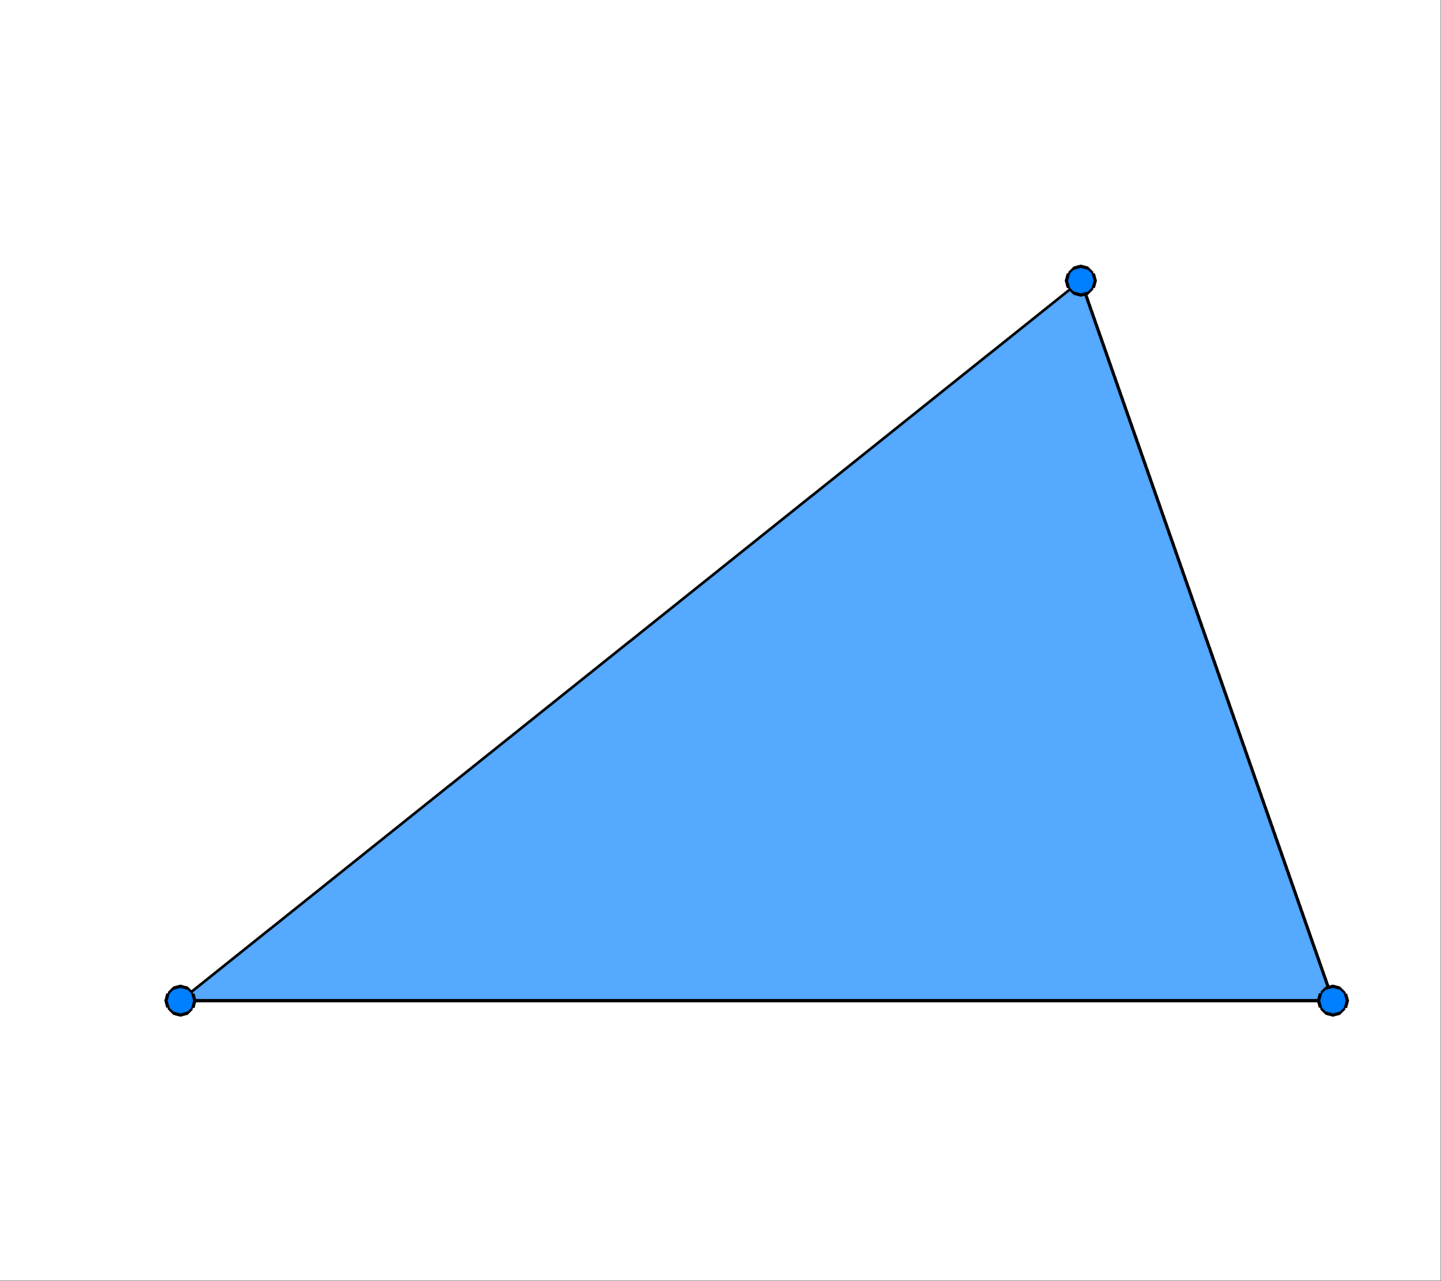
\includegraphics[trim={5cm 9cm 3cm 8cm},clip,width=0.29\textwidth]{FIGURES/LEVELSET_ARTICLE/TRI_ALL_NEG.png}
        \label{fig:TriAllNeg}%
    }
    \hspace{0.02\textwidth}
    \subfloat[2 negative nodes.]{%
        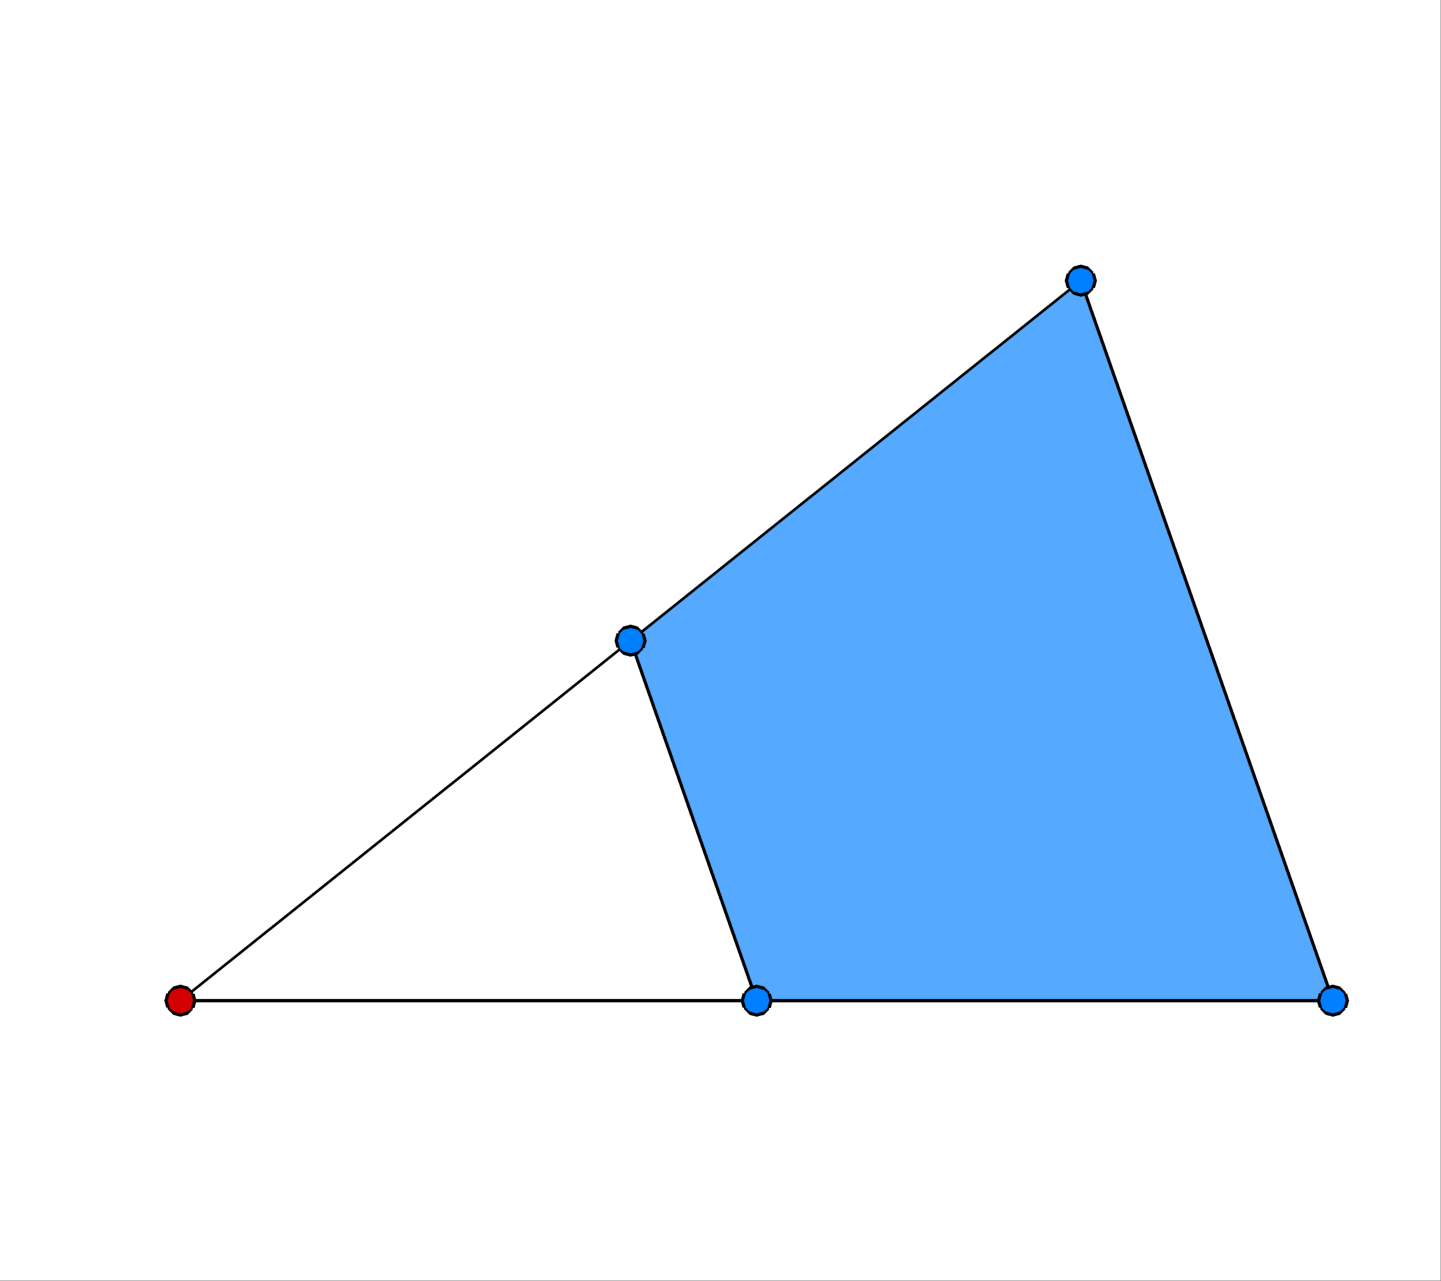
\includegraphics[trim={5cm 9cm 3cm 8cm},clip,width=0.29\textwidth]{FIGURES/LEVELSET_ARTICLE/TRI_TWO_NEG.png}
        \label{fig:TriTwoNeg}%
    }
    \hspace{0.02\textwidth}
    \subfloat[1 negative node.]{%
        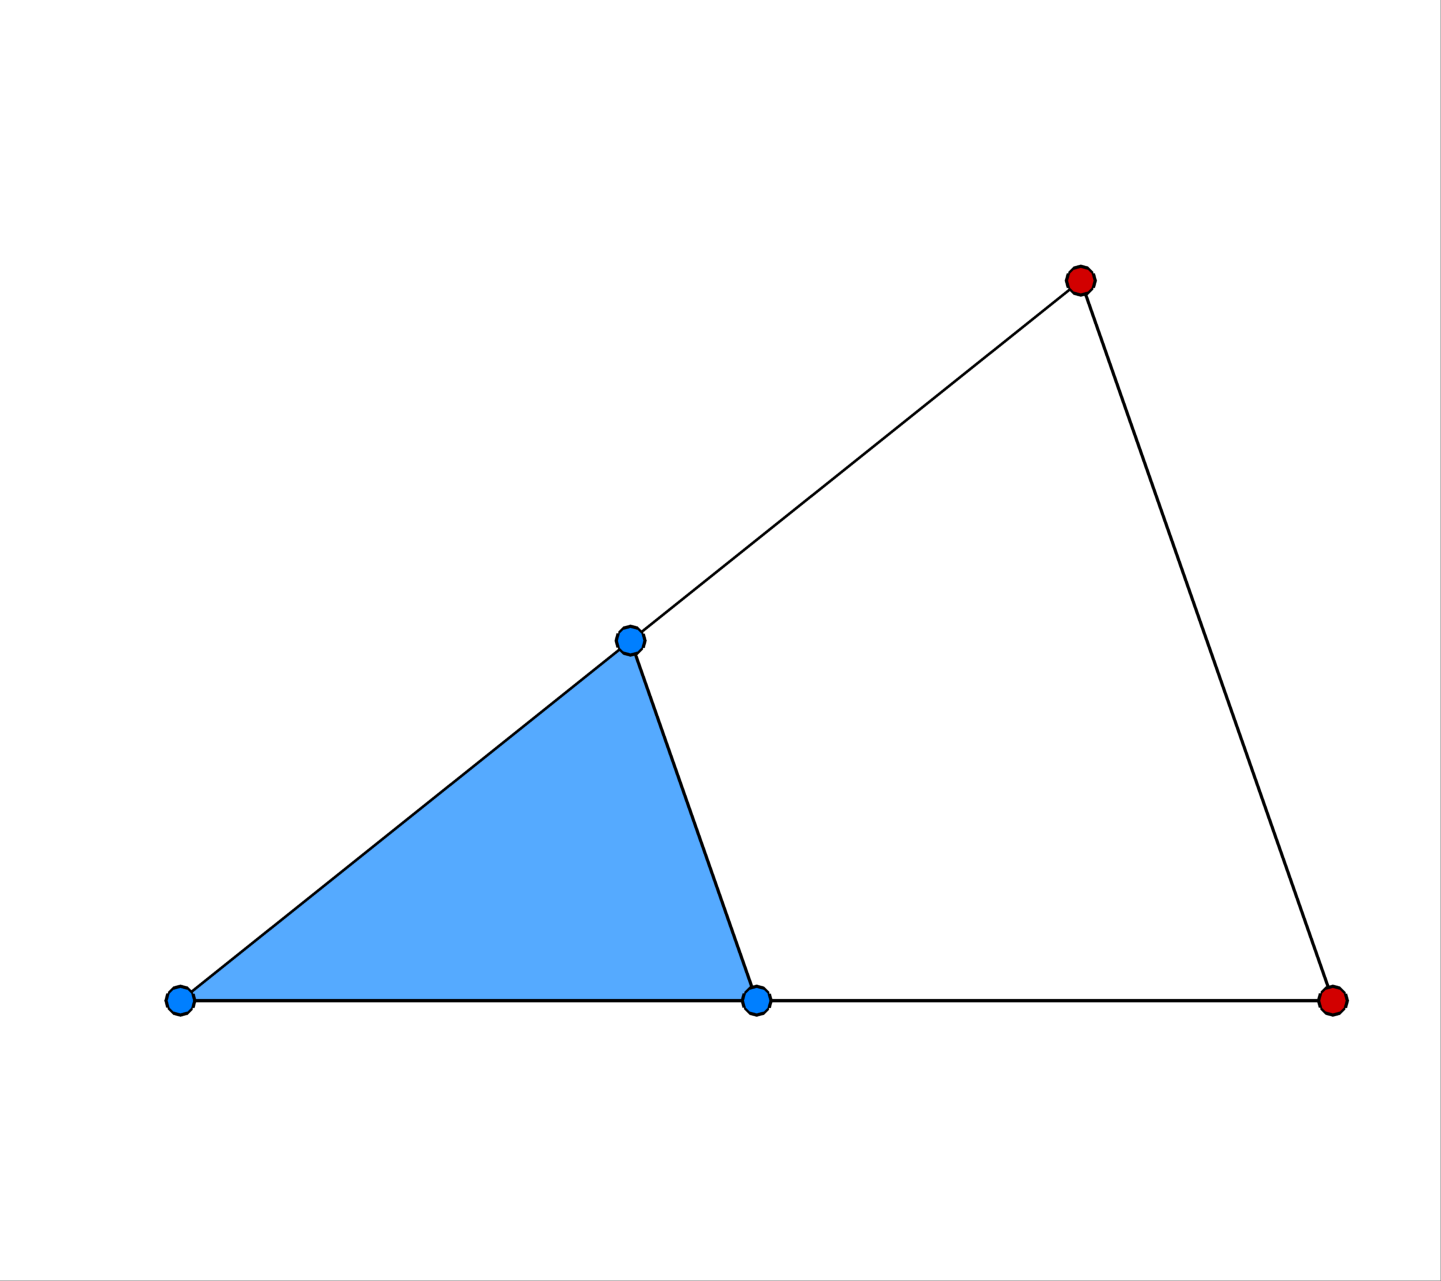
\includegraphics[trim={5cm 9cm 3cm 8cm},clip,width=0.29\textwidth]{FIGURES/LEVELSET_ARTICLE/TRI_ONE_NEG.png}
        \label{fig:TriOneNeg}%
    }

    \vspace{0.4cm}

    \subfloat[Fully negative tetrahedron.]{%
        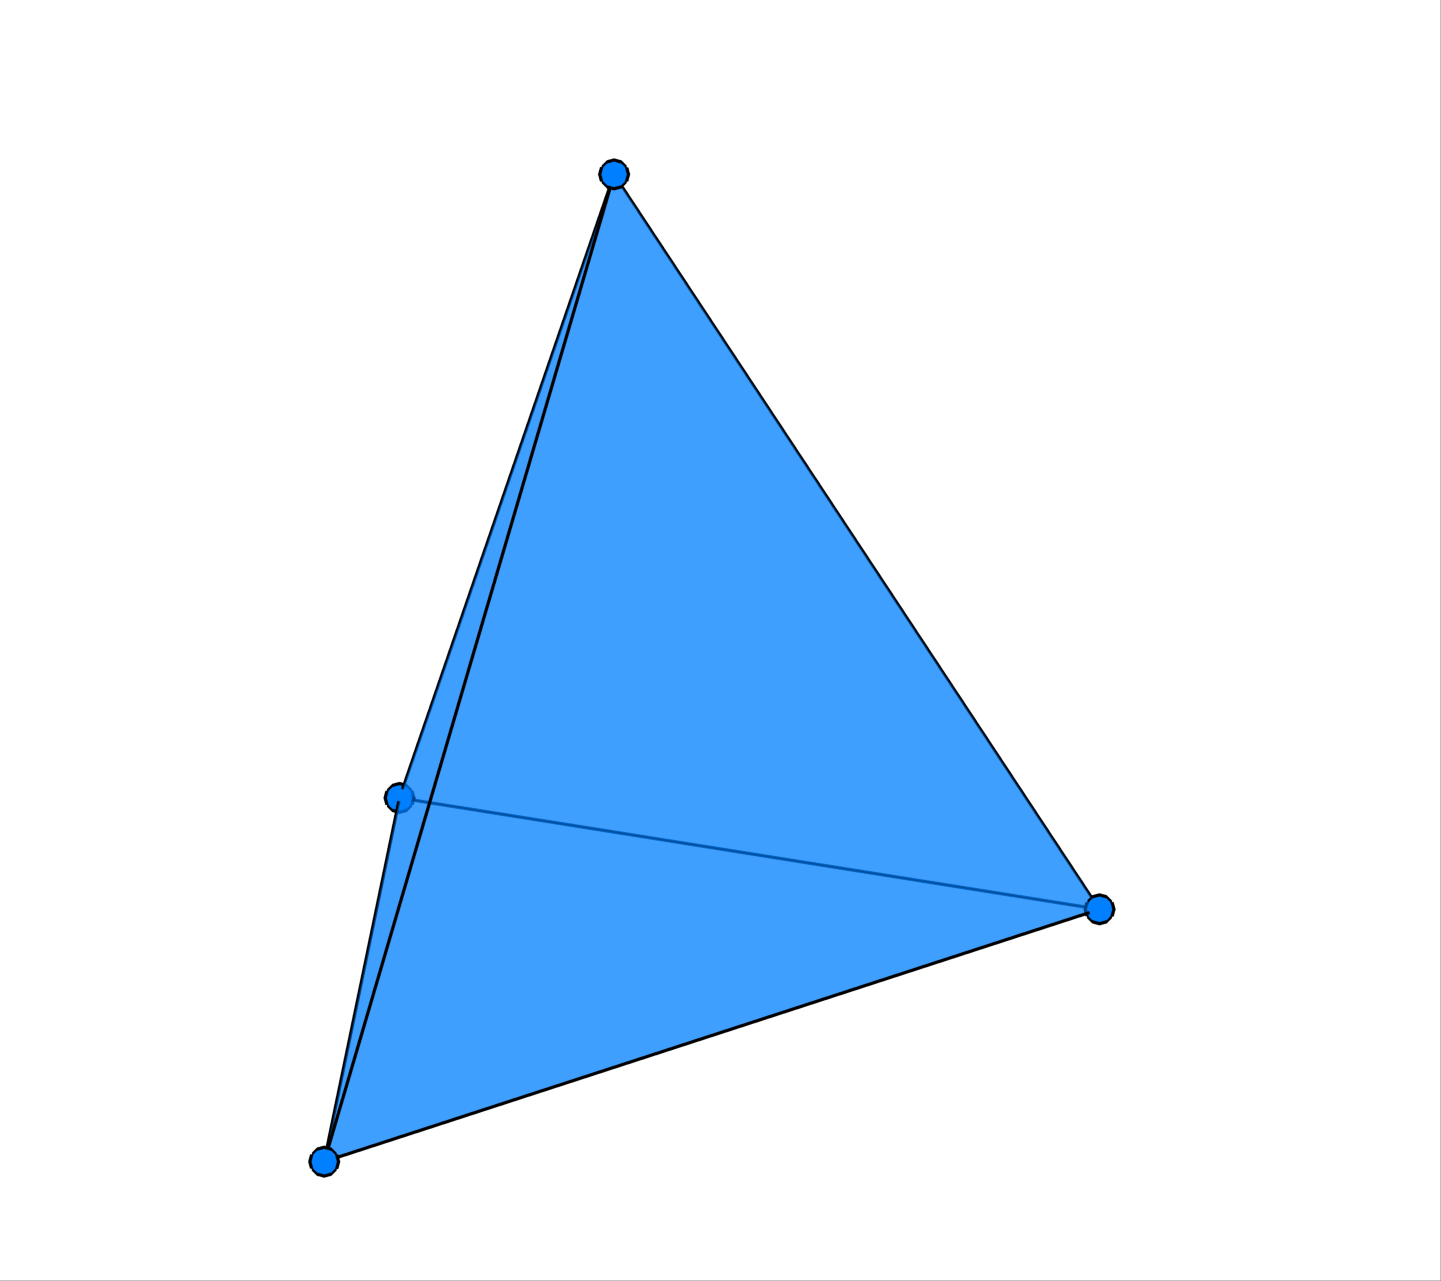
\includegraphics[trim={5cm 3cm 3cm 5cm},clip,width=0.22\textwidth]{FIGURES/LEVELSET_ARTICLE/TETRA_ALL_NEG.png}
        \label{fig:TetraAllNeg}%
    }
    \hspace{0.01\textwidth}
    \subfloat[3 negative nodes.]{%
        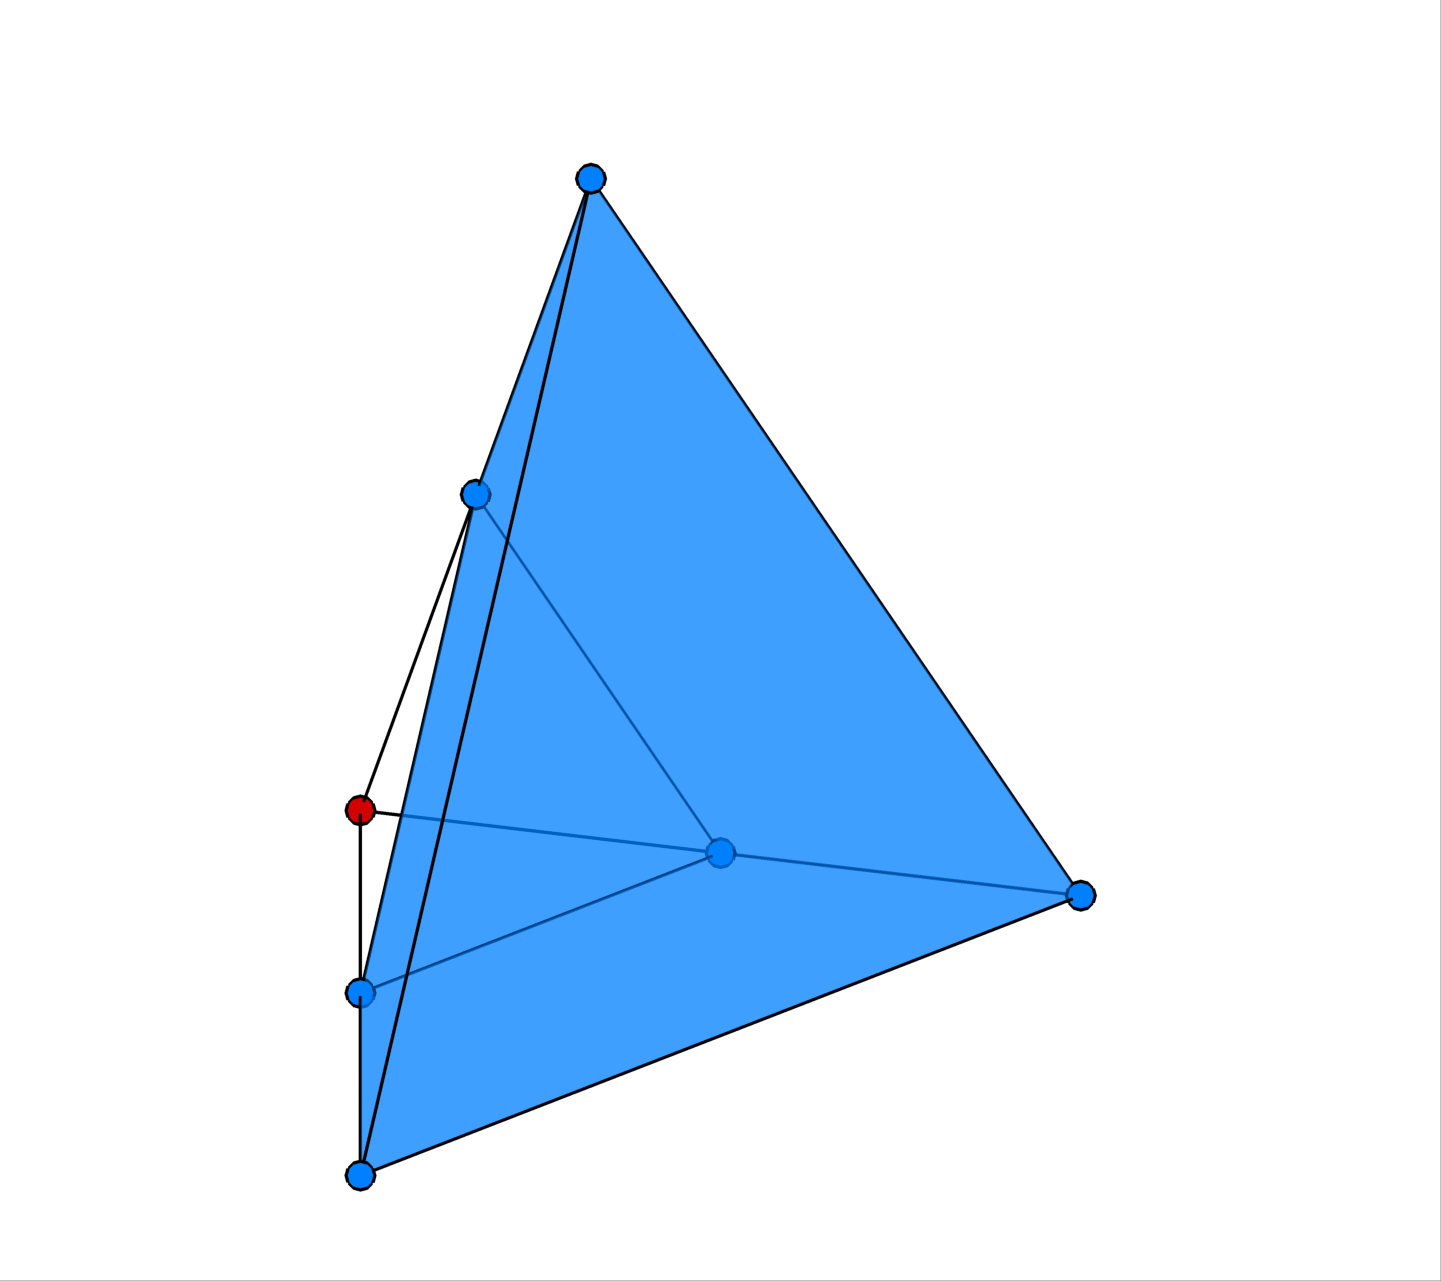
\includegraphics[trim={5cm 3cm 3cm 5cm},clip,width=0.22\textwidth]{FIGURES/LEVELSET_ARTICLE/TETRA_THREE_NEG.png}
        \label{fig:TetraThreeNeg}%
    }
    \hspace{0.01\textwidth}
    \subfloat[2 negative nodes.]{%
        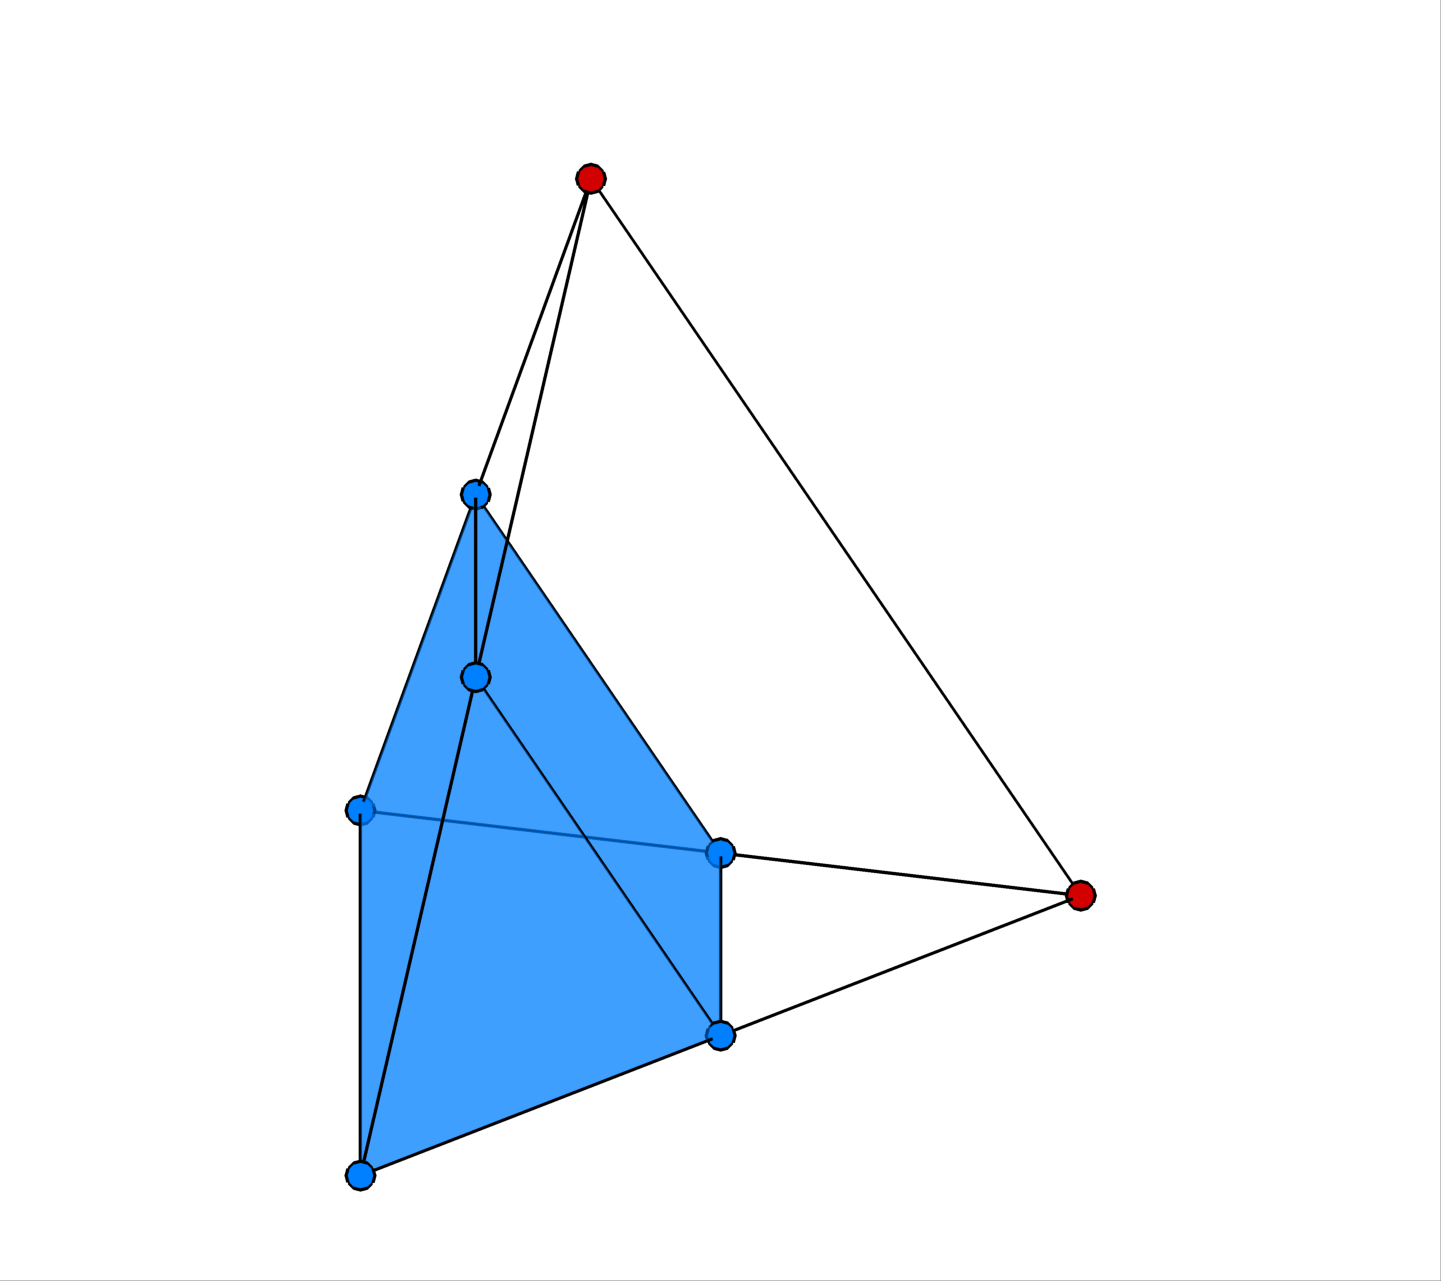
\includegraphics[trim={5cm 3cm 3cm 5cm},clip,width=0.22\textwidth]{FIGURES/LEVELSET_ARTICLE/TETRA_TWO_NEG.png}
        \label{fig:TetraTwoNeg}%
    }
    \hspace{0.01\textwidth}
    \subfloat[1 negative node.]{%
        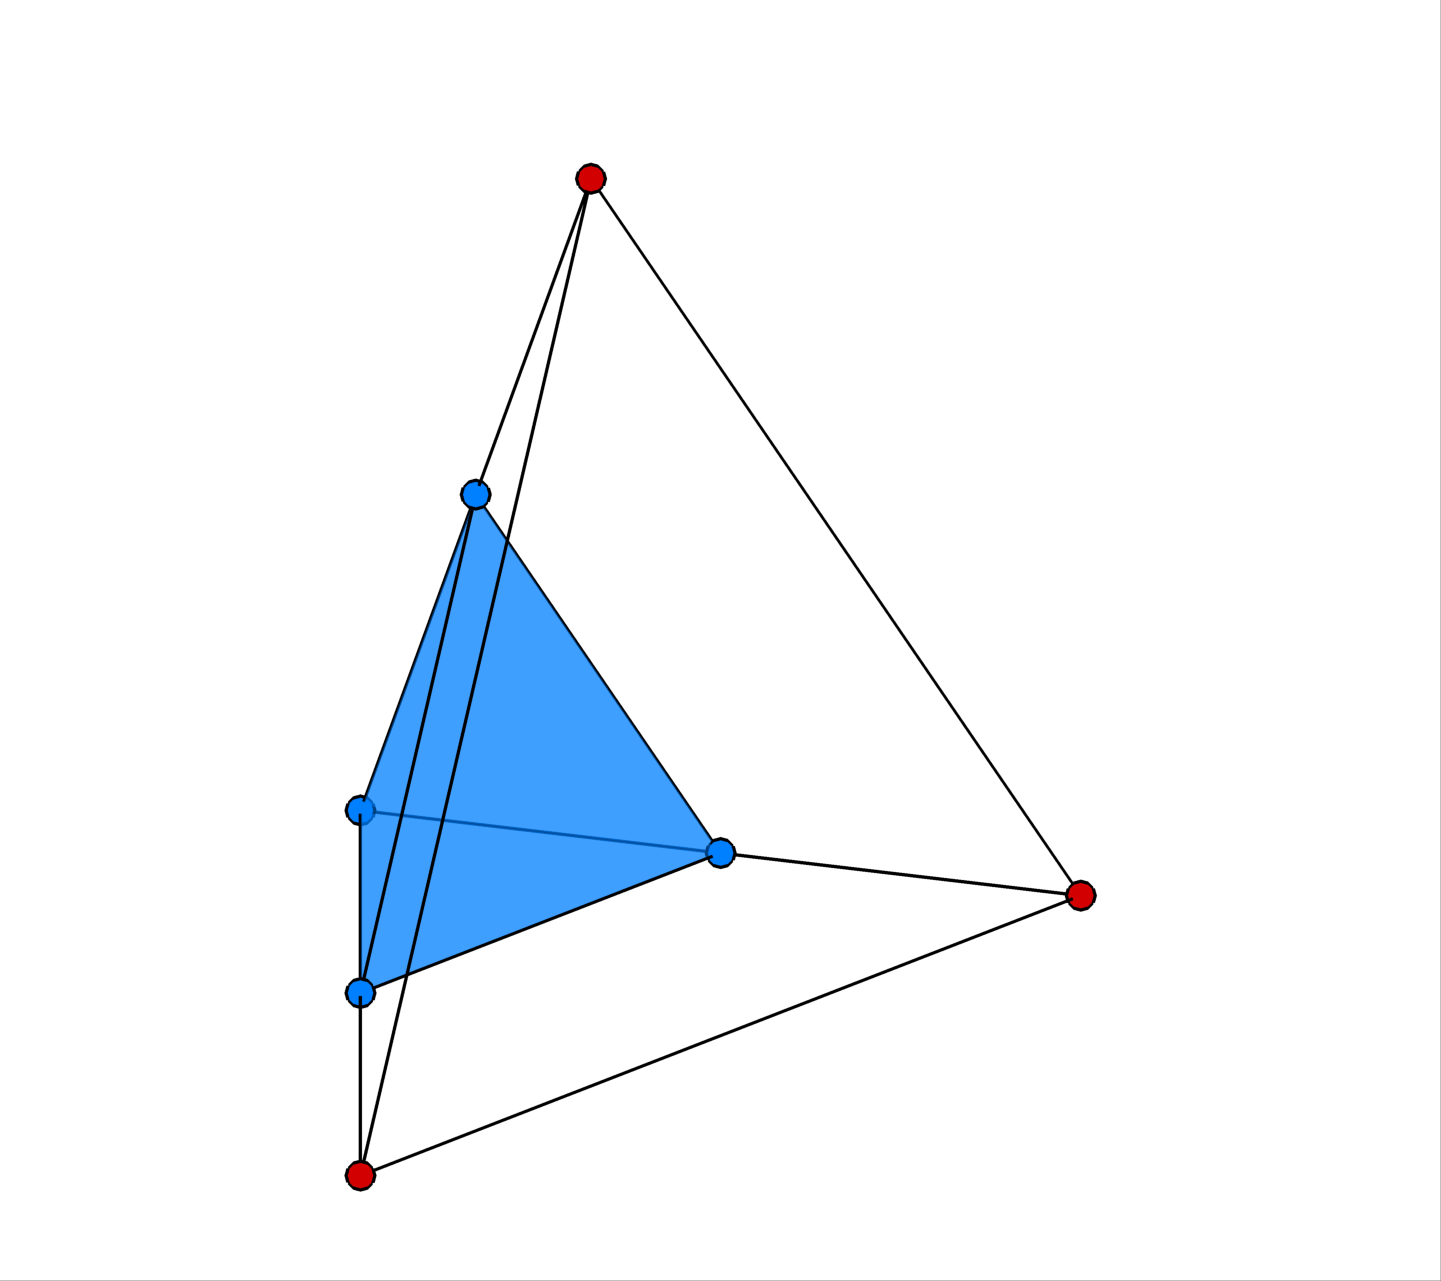
\includegraphics[trim={5cm 3cm 3cm 5cm},clip,width=0.22\textwidth]{FIGURES/LEVELSET_ARTICLE/TETRA_ONE_NEG.png}
        \label{fig:TetraOneNeg}%
    }

    \caption{Illustration of local interface reconstruction within simplicial elements based on the sign of the level-set function $\phi$. Red nodes denote positive values ($\phi>0$), whereas blue nodes denote negative values ($\phi<0$). The interface $\phi=0$ is reconstructed by linear interpolation along the intersected edges. In 2D, the negative subregion is either the full triangle, a quadrilateral, or a triangle. In 3D, the negative subregion is either the full tetrahedron, a truncated tetrahedron, a clipped polyhedron, or a smaller tetrahedral subregion. These clipped regions are used to evaluate the local ice area or volume contribution without requiring a full surface extraction.}
    \label{fig:LocalExtraction}
\end{figure}


\section{Geometry Extraction and Smoothing}
\label{sec:geometry_processing}

One of the main limitations reported in \cite{bourgault2019ice} was related to the RANS mesh, which constituted a restrictive aspect of the level-set simulation framework. Although the mesh was sufficiently refined to satisfy the $y^+ < 1$ requirement of the Spalart–Allmaras turbulence model, it was not well suited for the level-set formulation. In particular, the very fine near-wall cells imposed highly restrictive time-step constraints for the level-set advection, making the evolution of the interface computationally demanding. Furthermore, the geometry tracking was performed using a Lagrangian approach, which required heuristic procedures to handle topological events such as merging or breaking of the interface.

To address these limitations, the present study adopts a framework that generates adapted meshes for solving the level-set formulation. The constructed mesh accounts for both the geometry extents and the maximum ice thickness predicted by the thermodynamic model, thereby limiting the overall element count. In order to improve the accuracy of the continuous level-set tracking and extraction, the mesh is refined in regions where ice accretion occurs to reach a user-prescribed target element size. These regions are identified based on the condition $\dot{m}_{ice} > 0.0$. In addition, a set of transition layers is introduced to ensure a smooth transition between iced and clean regions of the geometry. The auxiliary grid is generated using MMG in 2D cases and through a \textsc{Pointwise} script \cite{fidelity_pointwise_2025} in 3D cases. An example of this adapted mesh is shown in Figure~\ref{fig:adaptedMesh}.

\begin{figure}[htbp] 
    \centering
    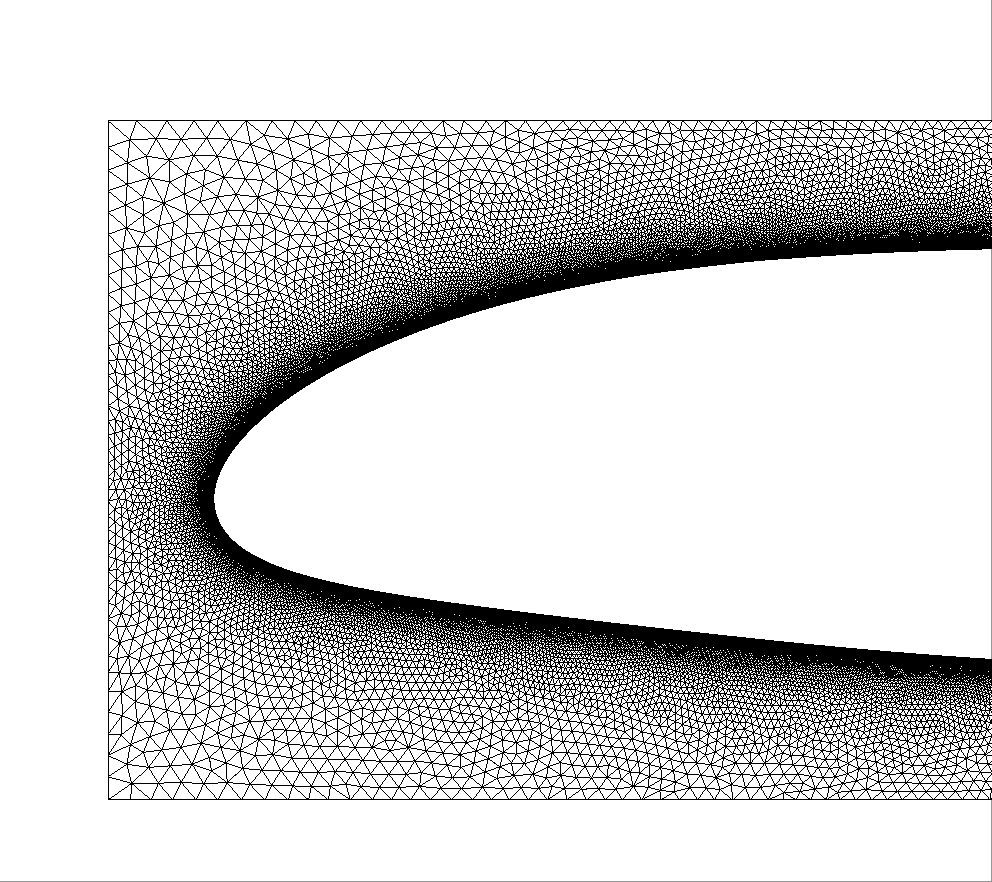
\includegraphics[trim={1cm 1cm 1cm 1cm}, clip, width=0.5\textwidth]{FIGURES/LEVELSET_ARTICLE/MESH_ADAPTATION.png}
    \caption{Adapted unstructured mesh around the iced surface of the geometry, showing local refinement in order to accurately capture the interface in the level-set framework.}
    \label{fig:adaptedMesh}
\end{figure}

An important aspect of the procedure is the preservation of the original clean geometry. Based on the previously defined accretion criterion, nodes and edges belonging to regions without ice accumulation are tagged as required entities so that they remain unaltered during the \textsc{MMG} adaptation/extraction process. Moreover, as the adapted surface mesh does not share the same discretization as the original surface in the iced regions, an interpolation step is required. This is performed using a linear interpolation by locating the closest element on the original surface mesh.

Once this mapping step is completed, the level-set framework is initiated by computing the eikonal $\phi$ and normals, propagating surface variables into the volume along these normals, and subsequently advecting the unsteady level-set field. Prior to extracting the geometry, the level-set values must be defined at mesh nodes since \textsc{MMG} operates on nodal values. Therefore, a final interpolation step is performed to transfer the cell-centered solution of the CHAMPS solver to nodal values. The zero level set is then extracted to obtain the updated surface geometry, which is subsequently used to generate the volume grid for the next accretion layer.

Surface perturbations may arise during several stages of the ice accretion simulation process, including the level-set solution, the geometry extraction procedure, and even during the computation of the droplet collection efficiency. As reported in \cite{pabloThesis}, these perturbations can introduce small geometric oscillations on the extracted interface. If left untreated, such oscillations may amplify during subsequent accretion layers and eventually lead to numerical instabilities or undesirable topological artifacts in the evolving ice geometry.

To mitigate these issues, a smoothing step is applied to regularize the surface while preserving the physically relevant geometric features of the ice shape. In the case of surface variables such as the collection efficiency, the smoothing procedure must also preserve the overall distribution and magnitude of the quantities involved. An effective approach reported in \cite{pabloThesis} is the smoothing filter proposed in \cite{taubinFilter}, which is well suited for this purpose. Unlike classical Gaussian smoothing, which tends to introduce geometric shrinkage and consequently alters the predicted ice volume, the filter reported in \cite{taubinFilter} was specifically designed to minimize such shrinkage effects while still removing high-frequency surface noise. 

This smoothing method can be interpreted as a low-pass filter applied to the mesh geometry. It attenuates high-frequency perturbations while preserving the large-scale structure of the surface. The algorithm operates through two successive passes of Laplacian smoothing. In the first pass, node positions are updated using a positive scaling factor $\lambda$, which produces a smoothing effect similar to standard Laplacian smoothing. In the second pass, a corrective update is applied using a negative factor $\mu$, which counteracts the shrinkage introduced during the first step. The combined effect of these two passes suppresses high-frequency oscillations while maintaining the global shape and volume of the surface. The pass-band frequency controlling the filter behavior is defined as $k_{pb} = \frac{1}{\lambda} + \frac{1}{\mu}$. The same filtering procedure can also be applied to surface fields when regularization of field variables is required. In this work, the pass-band frequency was set to $k_{pb}=0.01$, with $\lambda=0.33$. The number of smoothing iterations ranged from 2 to 50.

Through this two-stage filtering process, this smoothing filter effectively regularizes the extracted surface while preserving the geometric integrity of the predicted ice shape, making it particularly suitable for multilayer ice accretion simulations where accumulated numerical noise could otherwise degrade the solution quality. An example is presented in Figure~\ref{fig:SmoothingEffects}.

\begin{figure}[ht!]
\hspace*{0cm}
    \subfloat[Smoothing effects on the first ice layer.]{%
    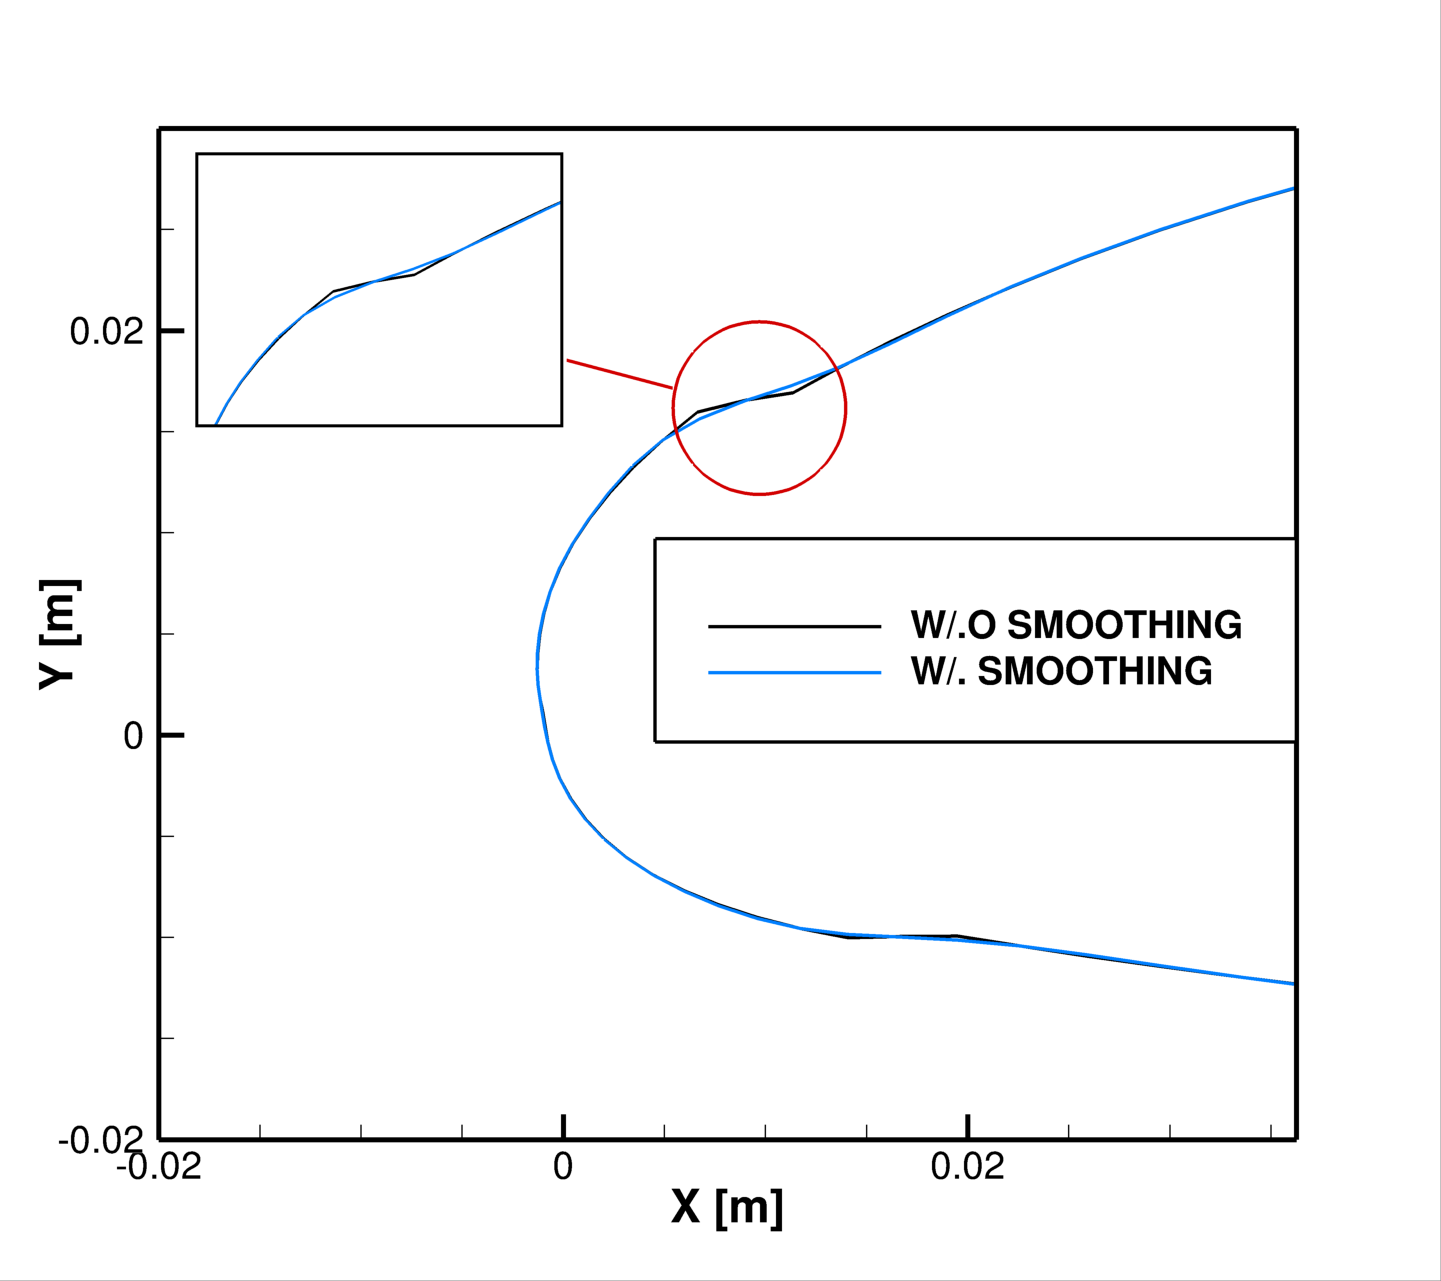
\includegraphics[trim={0cm 0cm 0cm 0cm},clip,width=0.5\textwidth]{FIGURES/LEVELSET_ARTICLE/SMOOTHING_EFFECTS_FIRST_LAYER.png}
    \label{fig:SmoothingEffectsFirstLayer}%
    }
    \hspace*{0.1cm}
    \subfloat[Smoothing effects on the final ice shape.]{%
    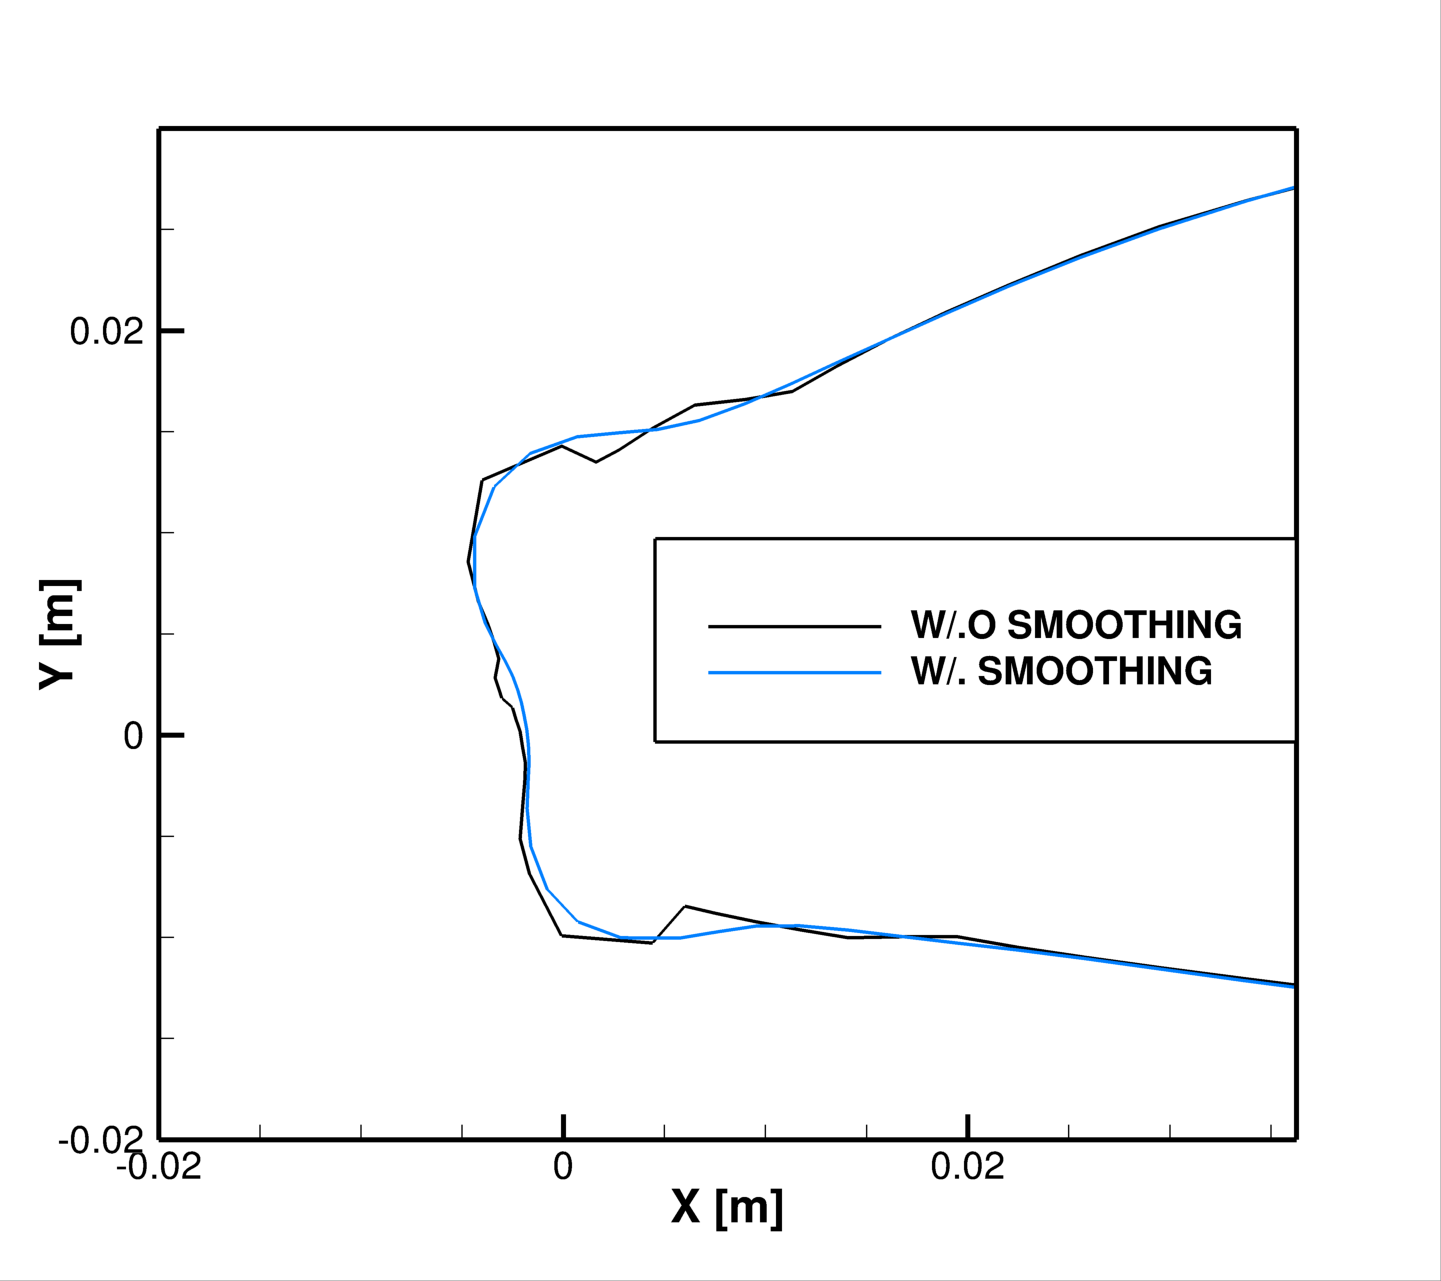
\includegraphics[trim={0cm 0cm 0cm 0cm},clip,width=0.5\textwidth]{FIGURES/LEVELSET_ARTICLE/SMOOTHING_EFFECTS_5_LAYERS.png}
    \label{fig:SmoothingEffects5Layer}%
    }
    \caption{Comparison of the effect of \cite{taubinFilter} smoothing on the extracted ice surface. Smoothing improves interface regularity in the first layer and prevents the accumulation of geometric distortions in the final ice shape.}
    \label{fig:SmoothingEffects}
\end{figure}

\section{Results}
\label{sec:results}

A primary objective of the present study is to assess the proposed level-set-based framework for ice accretion prediction on representative benchmark configurations, while also highlighting its advantages over a Lagrangian node-displacement approach in the presence of complex geometric features. To this end, a manufactured three-horn test case from \cite{lavoieLevelSet} is first considered to illustrate the ability of the level-set formulation to handle intricate interface evolutions and topological complexity that are more difficult to capture with explicit surface-node displacements. The numerical results are then evaluated on four cases drawn from the first Ice Prediction Workshop (IPW1, \cite{laurendeau2022summary}), namely Cases 241, 242, 361, and 362, as summarized in Table~\ref{tab:results}. The Ice Prediction Workshop (IPW) \cite{laurendeau2022summary,laurendeau2024summary} is a major international initiative organized by the American Institute of Aeronautics and Astronautics (AIAA) to evaluate and compare numerical tools for aircraft icing prediction against experimental data. It provides well-documented benchmark cases covering both 2D and 3D geometries under a variety of icing conditions.

Cases 241 and 242 correspond to 2D icing configurations on a NACA 23012 airfoil, whereas Cases 361 and 362 extend the analysis to a 3D configuration involving a swept NACA 0012 wing with a sweep angle of $30^\circ$. Together, these benchmark cases make it possible to evaluate the robustness of the proposed method on both 2D and 3D geometries, as well as its ability to capture a range of ice-shape features under different accretion conditions. Whenever available, the numerical results are compared with the experimental data and reference results provided within the IPW1 database. The experimental results are presented in the form of a maximum combined cross section (MCCS), obtained by extracting streamwise slices from the 3D scanned ice shape at multiple spanwise locations and combining these cross-sections into a single representation \cite{laurendeau2022summary}. Both the 3D scan and the corresponding MCCS data are available on the workshop website.

\begin{table}[ht]
\centering
\caption{Summary of the IPW1 benchmark cases.}
\begin{tabular}{ccccc}
\hline \hline
Parameter & 241 & 242 & 361 & 362 \\ 
\hline
Geometry & \makecell{2D\\NACA 23012} & \makecell{2D\\NACA 23012} & \makecell{3D Swept\\NACA 0012} & \makecell{3D Swept\\NACA 0012} \\
Icing Time [$min$] & 5.0 & 5.0 & 20.0 & 20.0 \\ 
LWC [$g/m^3$] & 0.42 & 0.81 & 0.5 & 0.5 \\ 
MVD [$\mu m$] & 30.0 & 15.0 & 34.7 & 34.7 \\ 
Ma [-] & 0.32 & 0.31 & 0.32  & 0.31 \\ 
AOA [\textdegree] & 2.0 & 2.0 & 0.0 & 0.0 \\ 
C$_{ref}$ [$inch$] & 18 & 18 & 36 & 36 \\ 
$T_{static}$ [$K$] & 250.15 & 266.05 & 257.0  & 266.0 \\  
Re [-] & $3.8 \cdot 10^6$ & $3.4 \cdot 10^6$ & $7.2 \cdot 10^6$ & $6.7 \cdot 10^6$ \\
\hline \hline
\end{tabular}
\label{tab:results}
\end{table}

\subsection{Three-Horns Ice Accretion Case}
\label{subsec:three_horns}

In order to highlight the capabilities of the level-set method, the first test case considered is the three-horns configuration initially introduced in \cite{lavoieThermo}. This manufactured case features three distinct ice horns, producing highly concave and convex regions that challenge interface tracking methods. An ice thickness of $0.02~\mathrm{m}$ is uniformly imposed on all surface nodes with $x < 0.05~\mathrm{m}$.

Figure~\ref{fig:ThreeHorns} compares the interface obtained from level-set contour extraction with that resulting from a Lagrangian node displacement approach. The latter exhibits clear limitations when handling the geometric complexity of the case. In particular, mesh entanglement is observed in regions of strong curvature, leading to local inconsistencies and ice mass loss, which explains the mismatch between the two predicted fronts. In contrast, the level-set method produces a smooth and conformal surface representation that remains robust in highly distorted regions. This allows for a consistent geometry extraction suitable for subsequent accretion layers, even in areas where the horns partially merge.

\begin{figure}[htbp] 
    \centering
    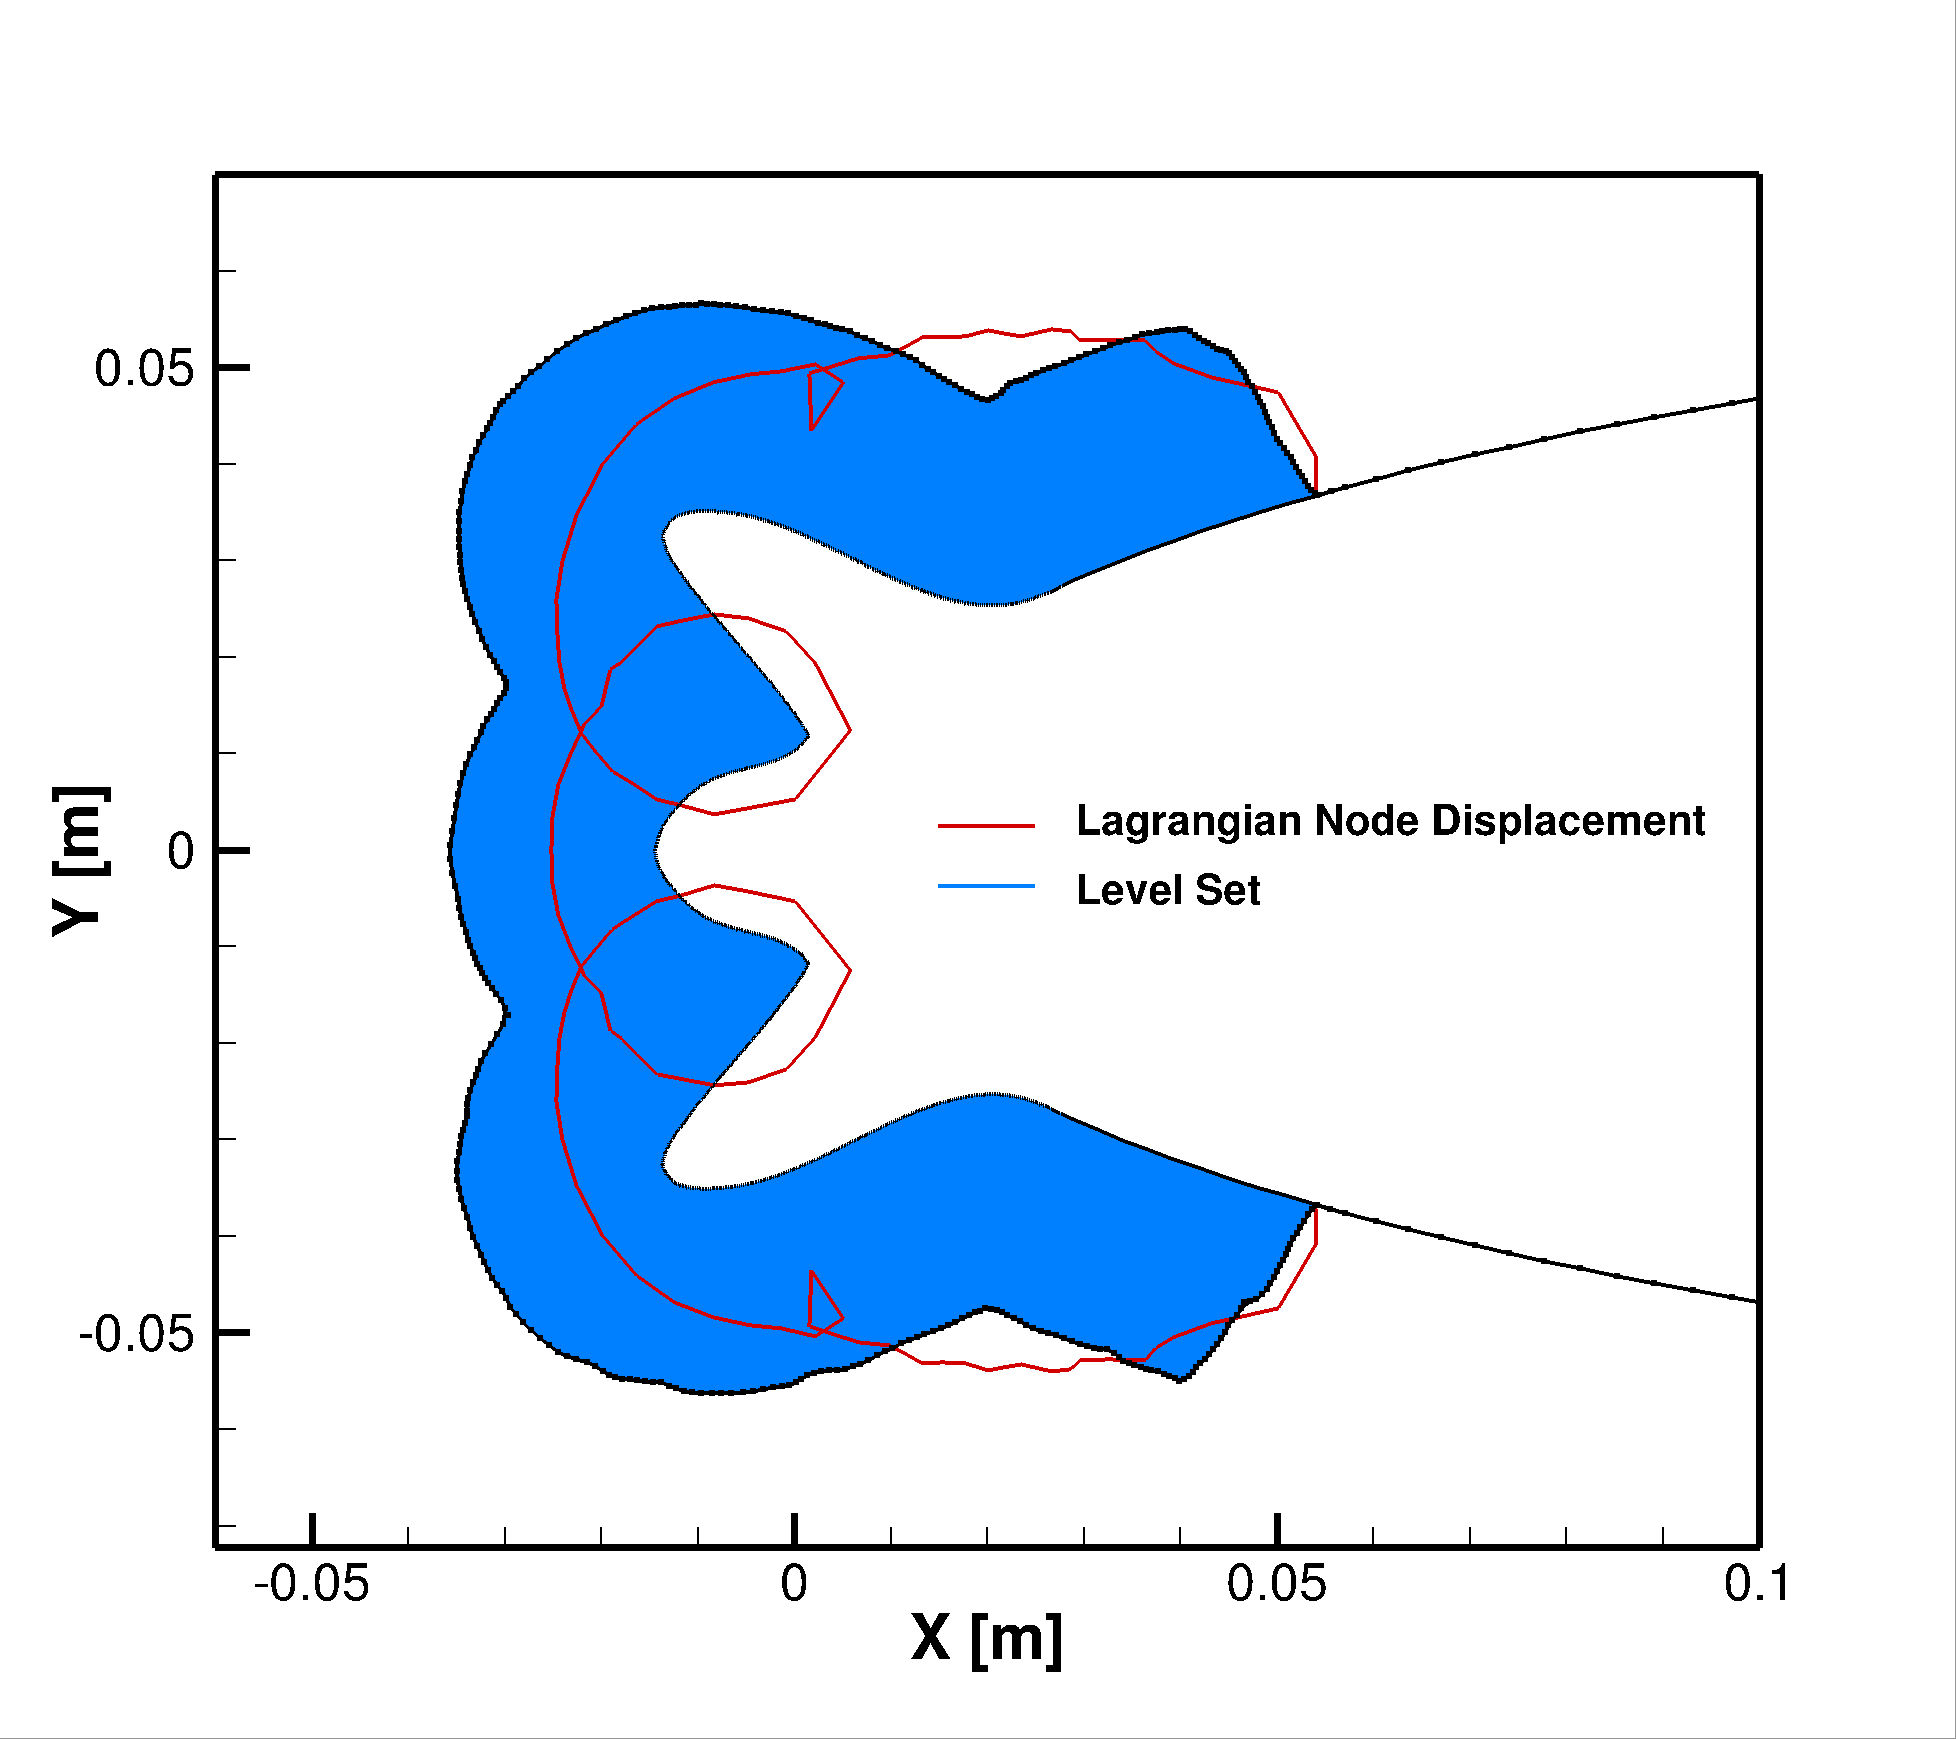
\includegraphics[trim={1cm 1cm 3cm 3cm}, clip, width=0.5\textwidth]{FIGURES/LEVELSET_ARTICLE/THREE_HORNS.png}
    \caption{Comparison of the ice fronts obtained using Lagrangian node displacement and the proposed level-set approach for the manufactured three-horn configuration.}
    \label{fig:ThreeHorns}
\end{figure}

\subsection{Case IPW1 241}
\label{subsec:naca_241}

The second case considered in this study corresponds to a rime ice case from IPW1. Rime ice forms when the temperature is significantly below the freezing point, such that water droplets freeze immediately upon impact. This leads to streamlined ice shapes. Figure~\ref{fig:Case241VariablesResults} presents the icing-related variables and compares them with the IPW1 participant results. Overall, the predicted distributions are in good agreement with the participant envelope. Figure~\ref{fig:Case241IceShape} shows the ice shape obtained for this case, again compared with the IPW1 results and with the experimental MCCS. The level-set solution agrees well with the experimental maximum ice height at the leading edge, with some mismatch on the upper and lower surfaces. These differences may be partly attributed to experimental uncertainties. Stochastic ice-accretion solvers reported in the literature, such as \cite{PAPILLONLAROCHE2023104420}, may provide improved predictions in these regions. Figure~\ref{fig:Case241IceShape} also shows the convergence of the ice shape with an increasing number of accretion layers for the level-set method, using 1, 10, and 20 layers. The solution is seen to converge by 10 layers, while the differences between 10 and 20 layers remain negligible.

\begin{figure}[ht!]
\hspace*{0cm}
    \subfloat[Pressure coefficient.]{%
    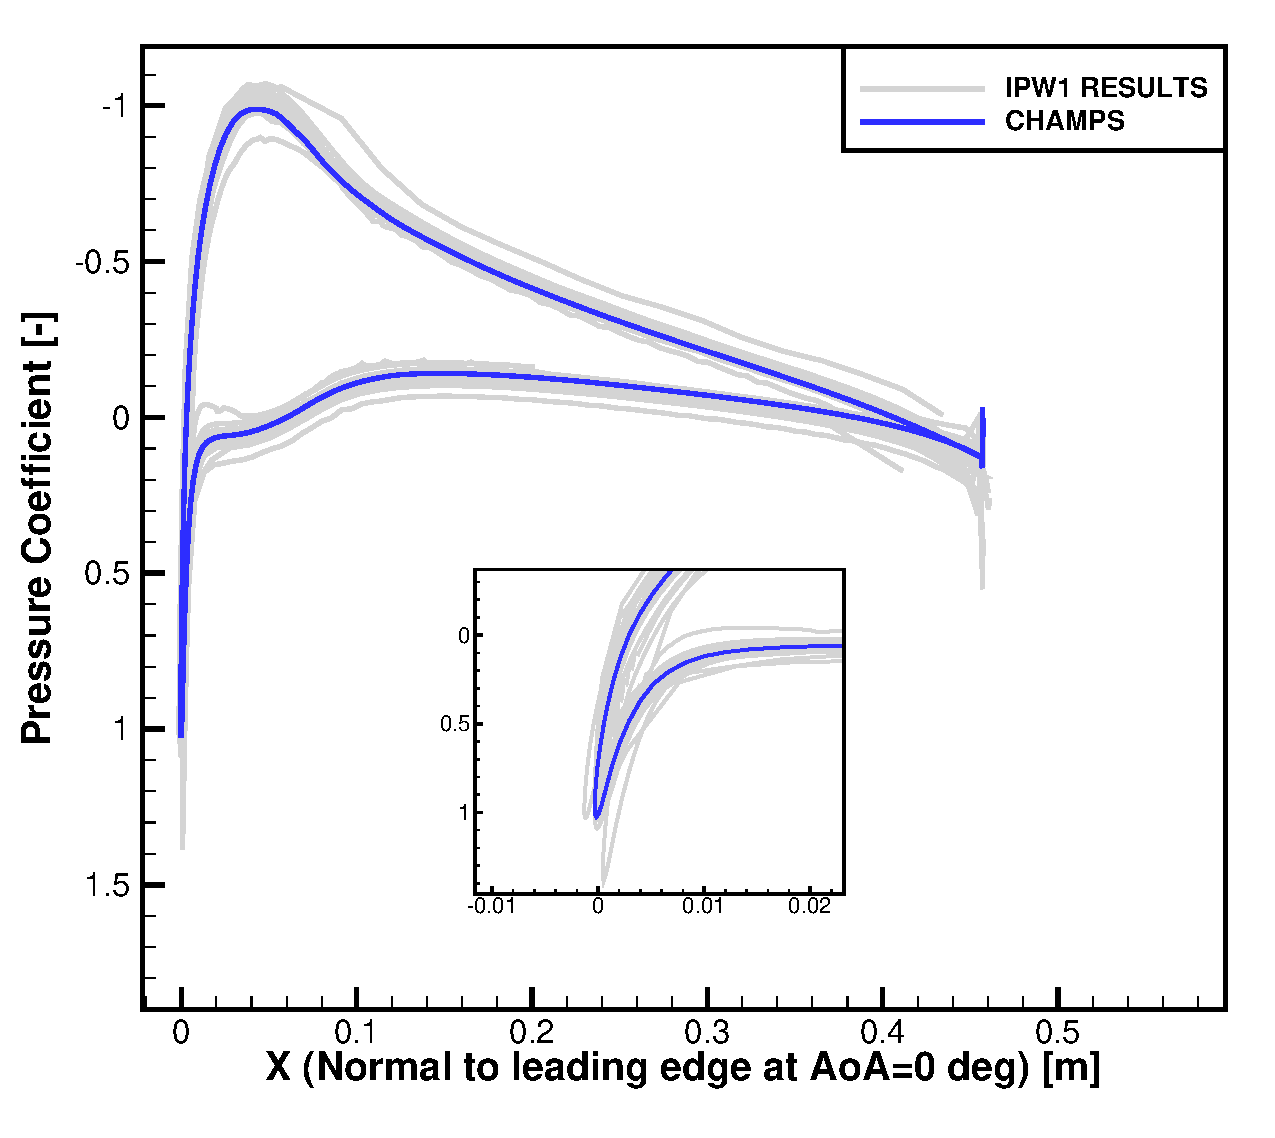
\includegraphics[trim={0cm 0cm 0cm 0cm},clip,width=0.32\textwidth]{FIGURES/LEVELSET_ARTICLE/CASE_IPW1_241_CP.eps}
    \label{fig:Case241Cp}%
    }
    \hspace*{0.1cm}
    \subfloat[Collection efficiency.]{%
    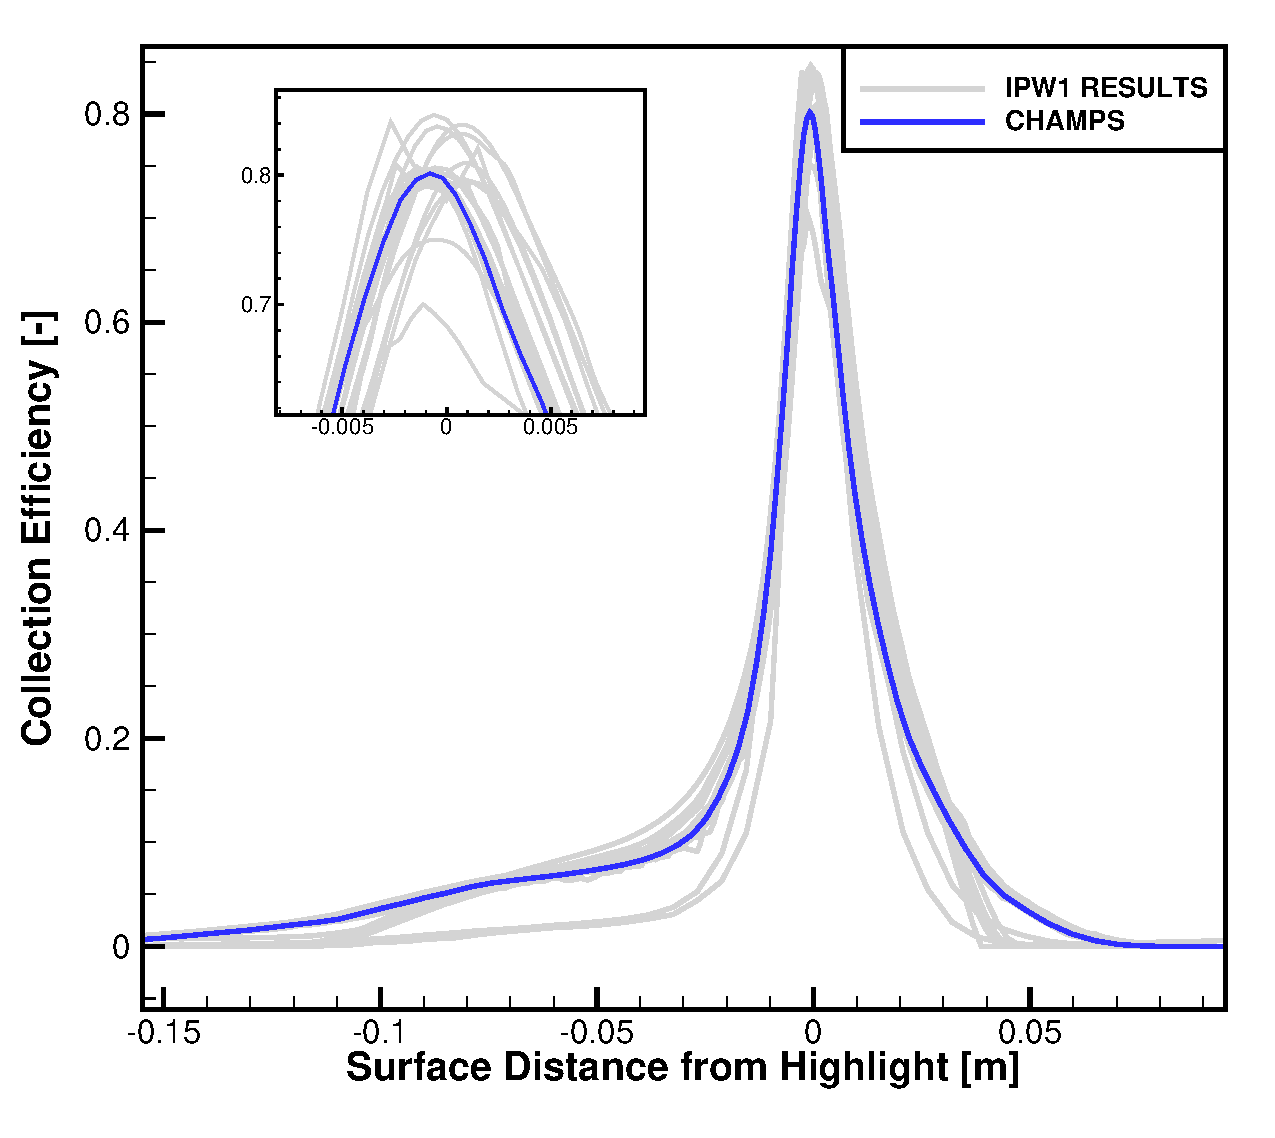
\includegraphics[trim={0cm 0cm 0cm 0cm},clip,width=0.32\textwidth]{FIGURES/LEVELSET_ARTICLE/CASE_IPW1_241_BETA.eps}
    \label{fig:Case241Beta}%
    }
    \hspace*{0.1cm}
    \subfloat[Convective heat transfer.]{%
    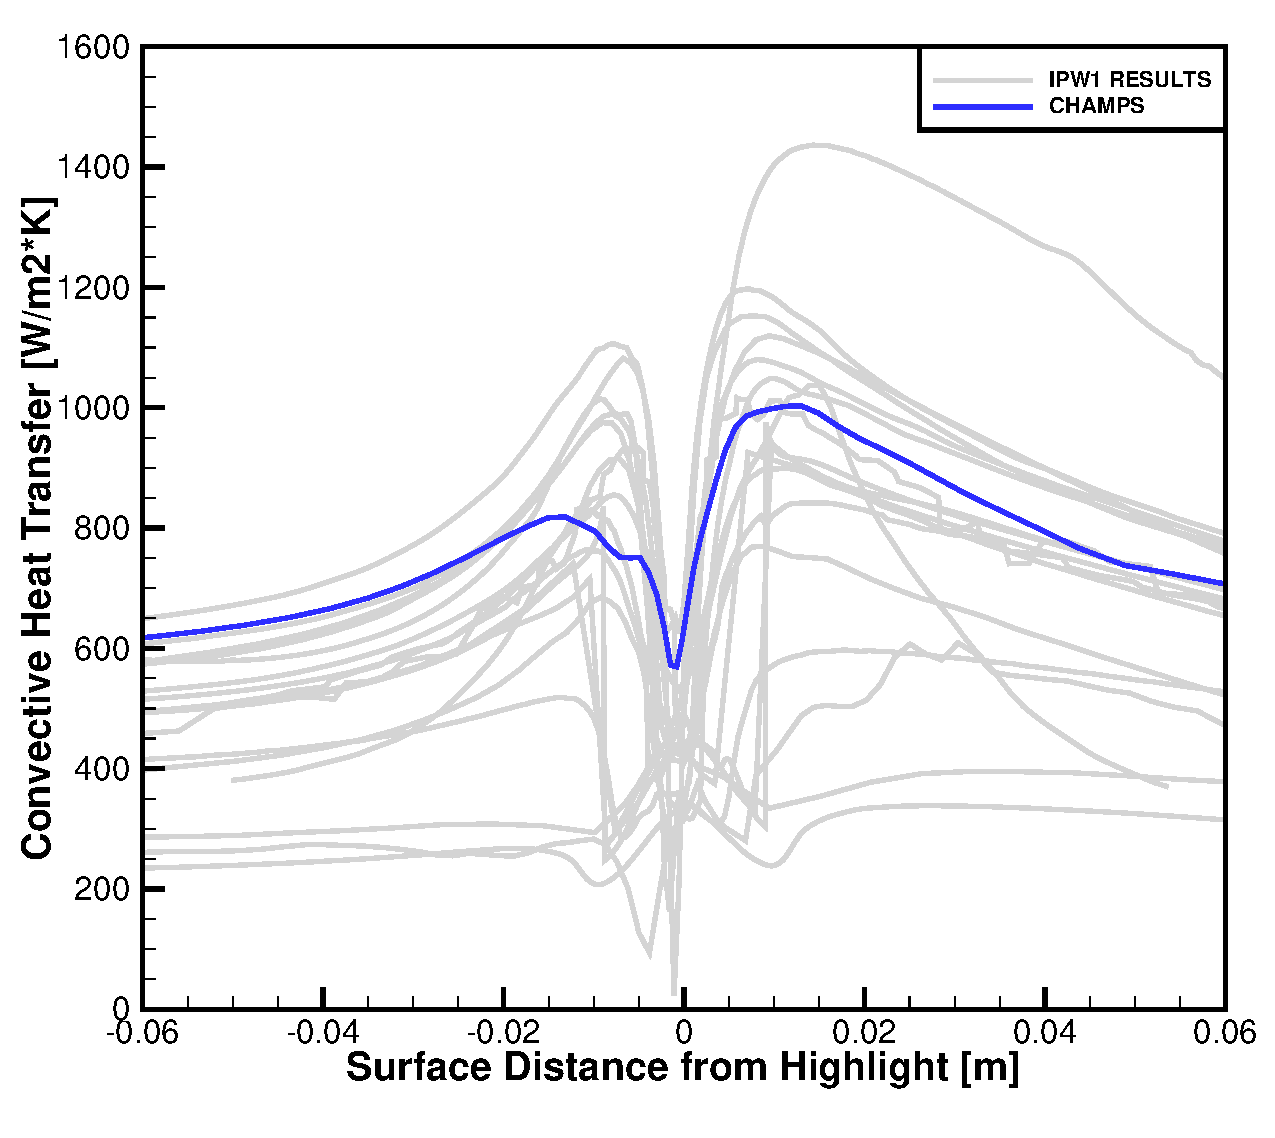
\includegraphics[trim={0cm 0cm 0cm 0cm},clip,width=0.32\textwidth]{FIGURES/LEVELSET_ARTICLE/CASE_IPW1_241_HTC.eps}
    \label{fig:Case241HTC}%
    }
    \caption{Comparison of the predicted aerodynamic and icing-related surface quantities for IPW1 Case 241 with the range of results submitted by IPW1 participants.}
    \label{fig:Case241VariablesResults}
\end{figure}

\begin{figure}[htbp] 
    \centering
    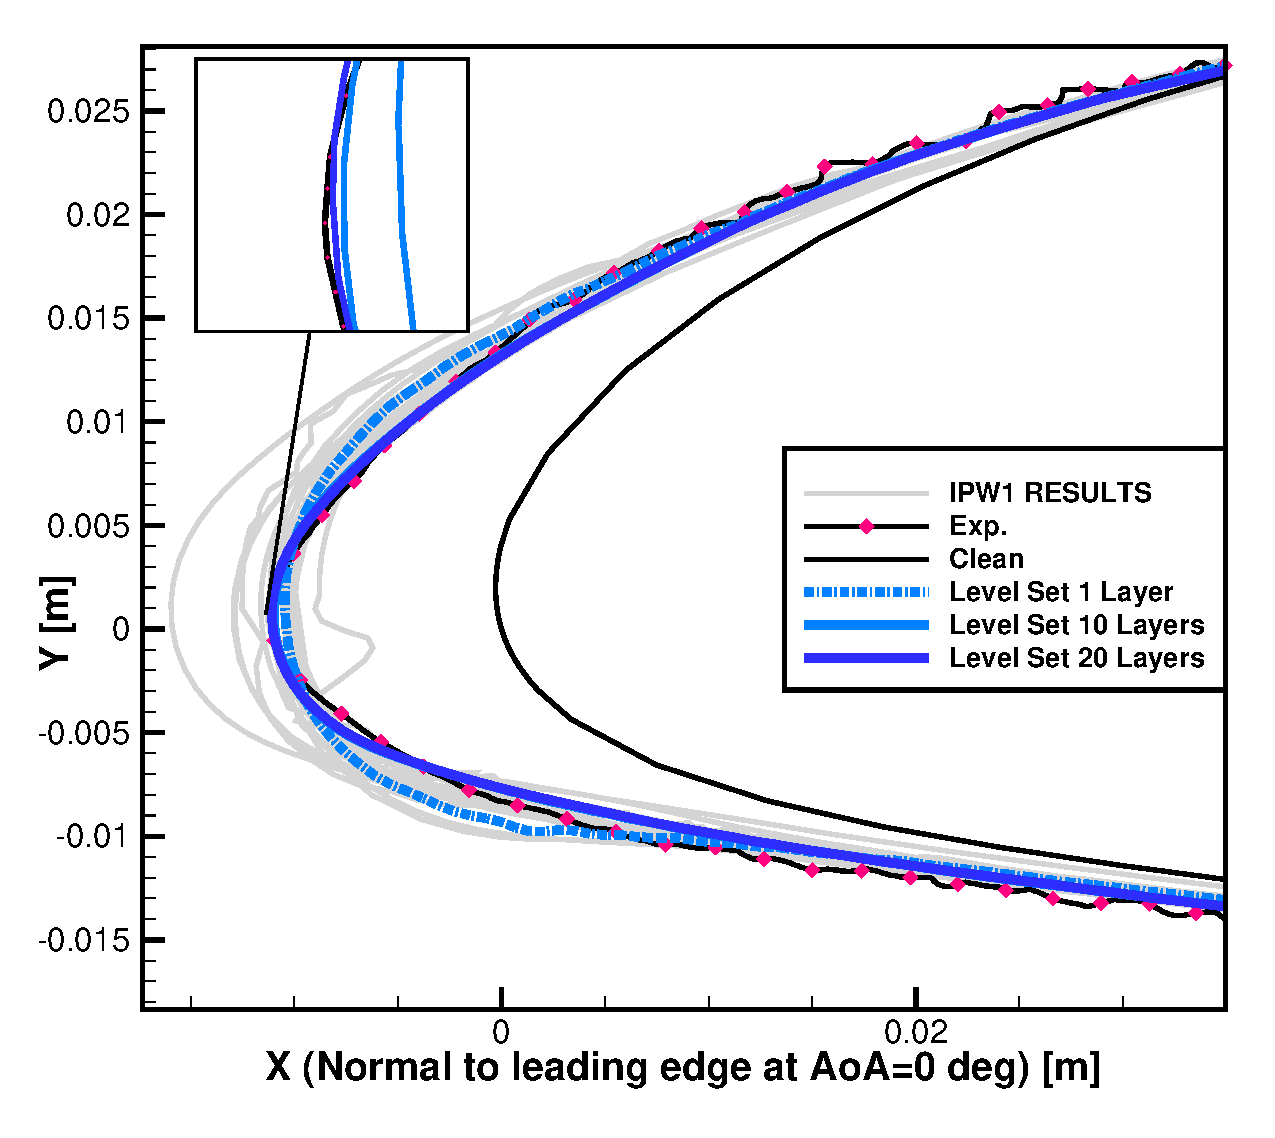
\includegraphics[trim={.1cm .1cm .1cm .1cm}, clip, width=0.5\textwidth]{FIGURES/LEVELSET_ARTICLE/CASE_IPW1_241_ICE_SHAPE.eps}
    \caption{Predicted ice shapes for IPW1 Case 241. The clean and experimental profiles are shown with the IPW1 participants' results. CHAMPS level-set predictions using 1, 10, and 20 accretion layers are included to assess the effect of the multilayer approach.}
    \label{fig:Case241IceShape}
\end{figure}

Ice shape comparisons remain difficult to assess in a fully quantitative manner, since the agreement between numerical and experimental accretions is often judged not only through global geometric measures but also through more qualitative considerations. In practice, validation therefore frequently relies on a combination of visual inspection and a limited number of representative geometric indicators. For the present rime ice case, no experimental ice mass data is available, which prevents the use of a direct mass-based comparison metric. Under these conditions, the maximum ice height at the leading edge constitutes a particularly relevant quantity for comparison, as it provides a simple and physically meaningful measure of the accretion. The values reported in Table~\ref{tab:maxIceHeightComparison} show that this metric is progressively improved as the number of accretion layers increases, with the relative error decreasing from 6.47$\%$ for the single-layer level-set prediction to 1.68$\%$ for the 10 layers simulation and 0.70$\%$ for the 20 layers simulation. These results indicate a clear convergence of the predicted rime ice shape toward the experimental reference with increasing temporal resolution of the multilayer accretion process.

\begin{table}[ht]
\centering
\caption{Comparison of the maximum ice height relative to the clean geometry.}
\begin{tabular}{lcc}
\hline \hline
Config. & Ice height [mm] & Relative error [\%] \\
\hline
Exp.   & $10.87$ & -- \\
01 layer   & $10.16$ & $6.47$ \\
10 layers & $10.69$ & $1.68$ \\
20 layers & $10.79$ & $0.70$ \\
\hline \hline
\end{tabular}
\label{tab:maxIceHeightComparison}
\end{table}

\subsection{Case IPW1 242}
\label{subsec:naca_242}
The third case considered is a glaze ice case, for which the static temperature is not sufficiently low to ensure immediate freezing upon droplet impact. As a result, a liquid water film forms on the surface, and part of the collected water runs back downstream before freezing. In contrast to rime ice, this process leads to less streamlined and more complex accreted shapes, often characterized by the development of ice horns \cite{diebold2013aerodynamic}. The icing-related variables obtained for this case are presented in Figure~\ref{fig:Case242VariablesResults}. Overall, the predicted trends remain in reasonable agreement with the range of results reported by the other IPW1 participants. However, the computed heat transfer coefficient (HTC) lies on the lower end of the participant spread, which is consistent with the formation of an ice shape that does not fully match the experimental accretion, as further illustrated in Figure~\ref{fig:iceShapeBaselineVsImproved}.

\begin{figure}[ht!]
\hspace*{0cm}
    \subfloat[Pressure coefficient.]{%
    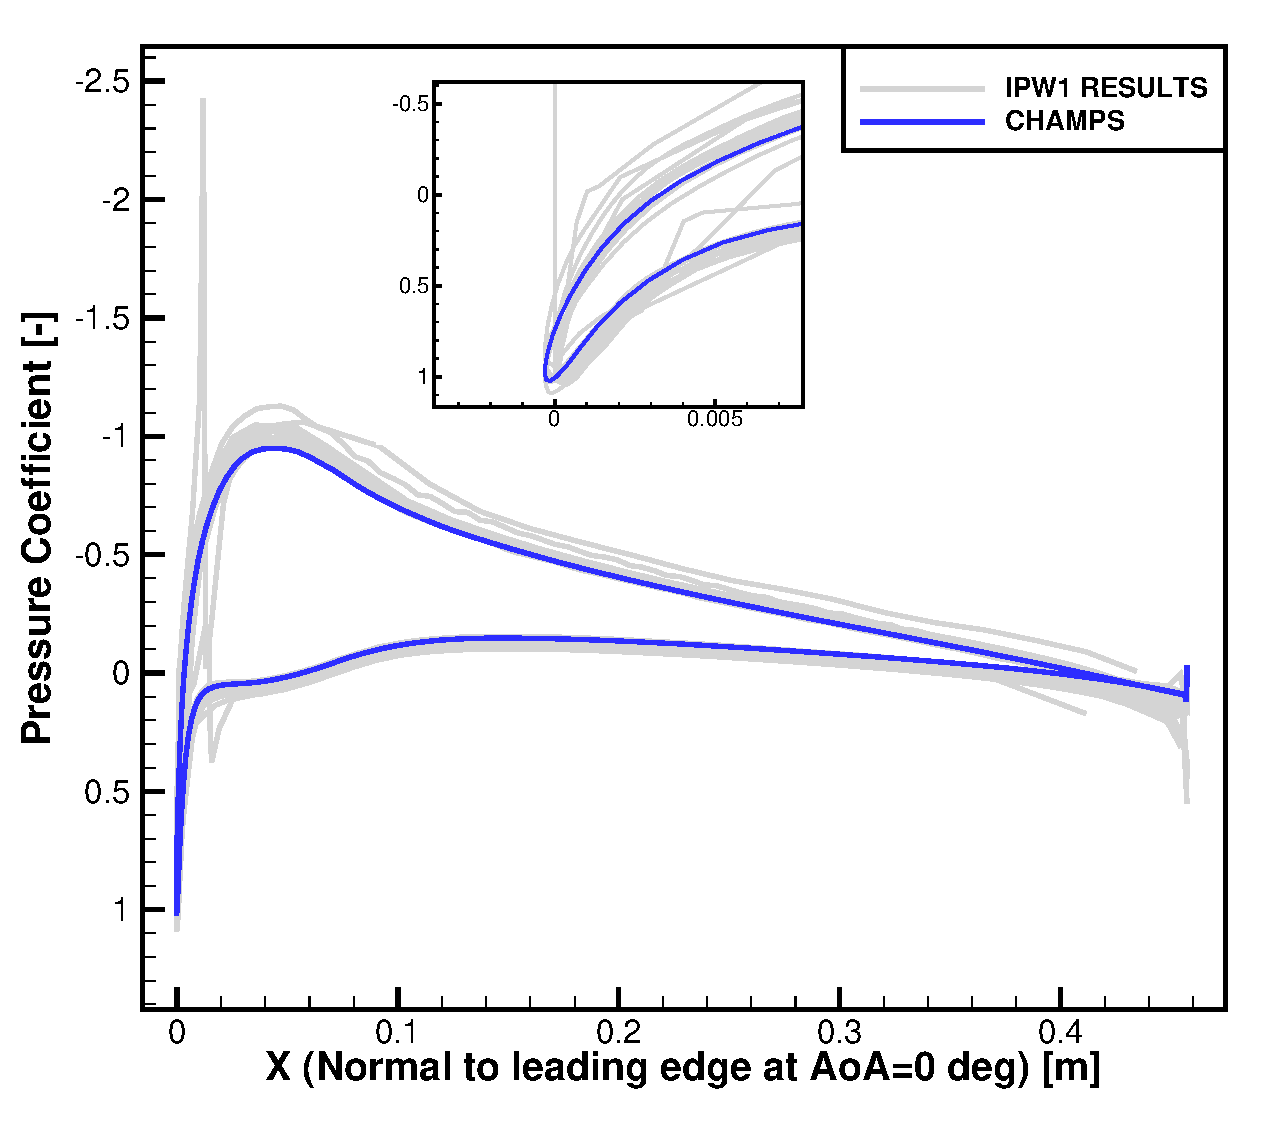
\includegraphics[trim={0cm 0cm 0cm 0cm},clip,width=0.32\textwidth]{FIGURES/LEVELSET_ARTICLE/CASE_IPW1_242_CP.eps}
    \label{fig:Case242Cp}%
    }
    \hspace*{0.1cm}
    \subfloat[Collection efficiency.]{%
    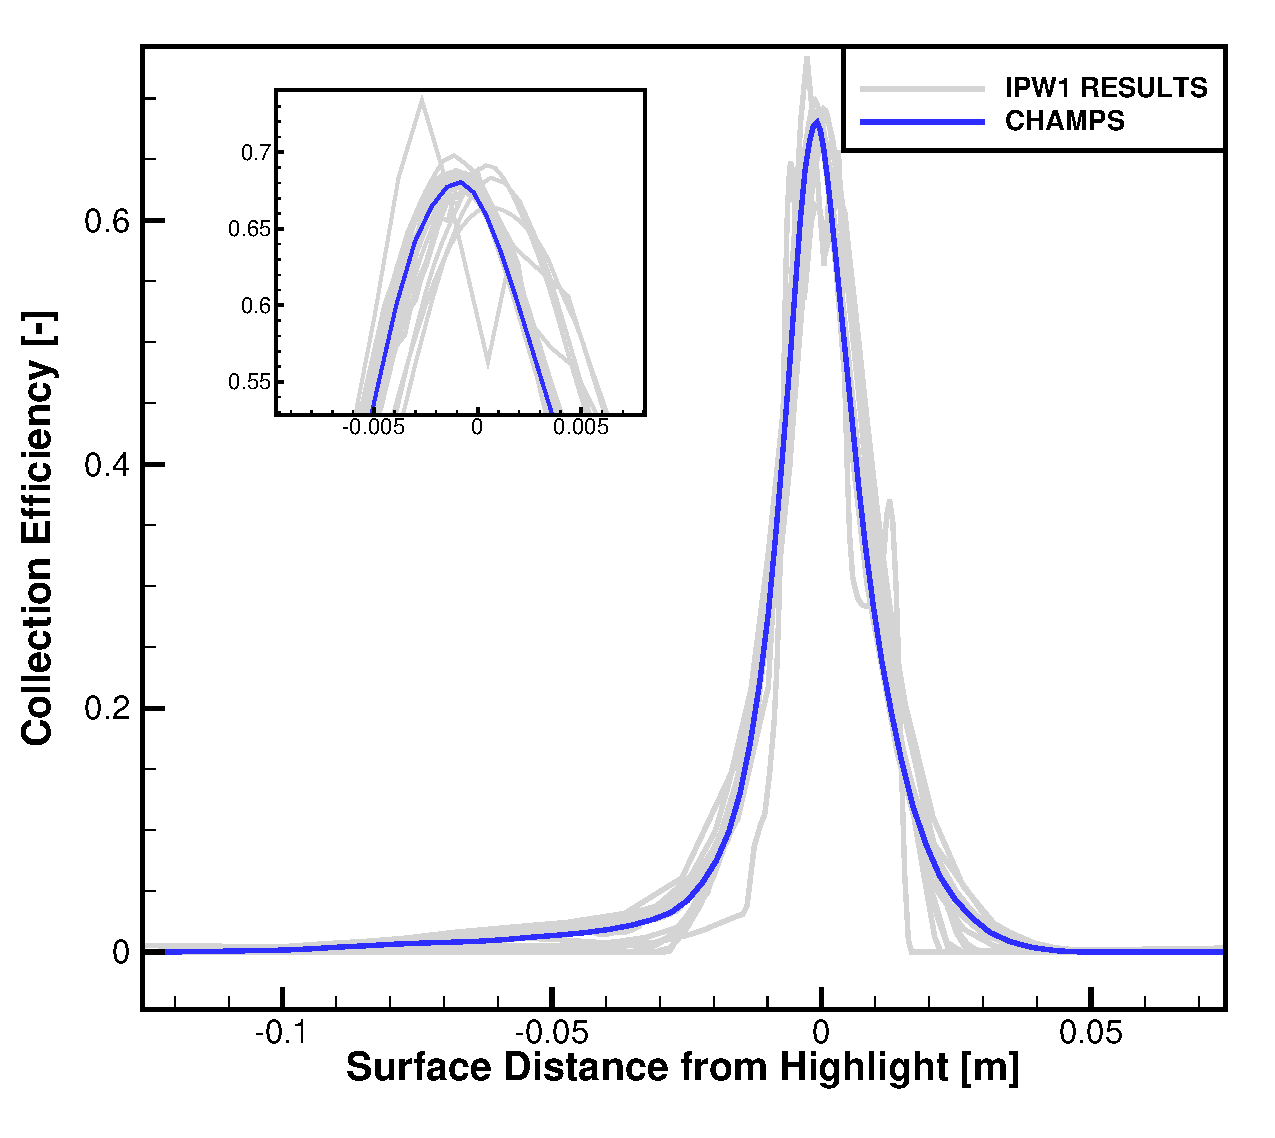
\includegraphics[trim={0cm 0cm 0cm 0cm},clip,width=0.32\textwidth]{FIGURES/LEVELSET_ARTICLE/CASE_IPW1_242_BETA.eps}
    \label{fig:Case242Beta}%
    }
    \hspace*{0.1cm}
    \subfloat[Convective heat transfer.]{%
    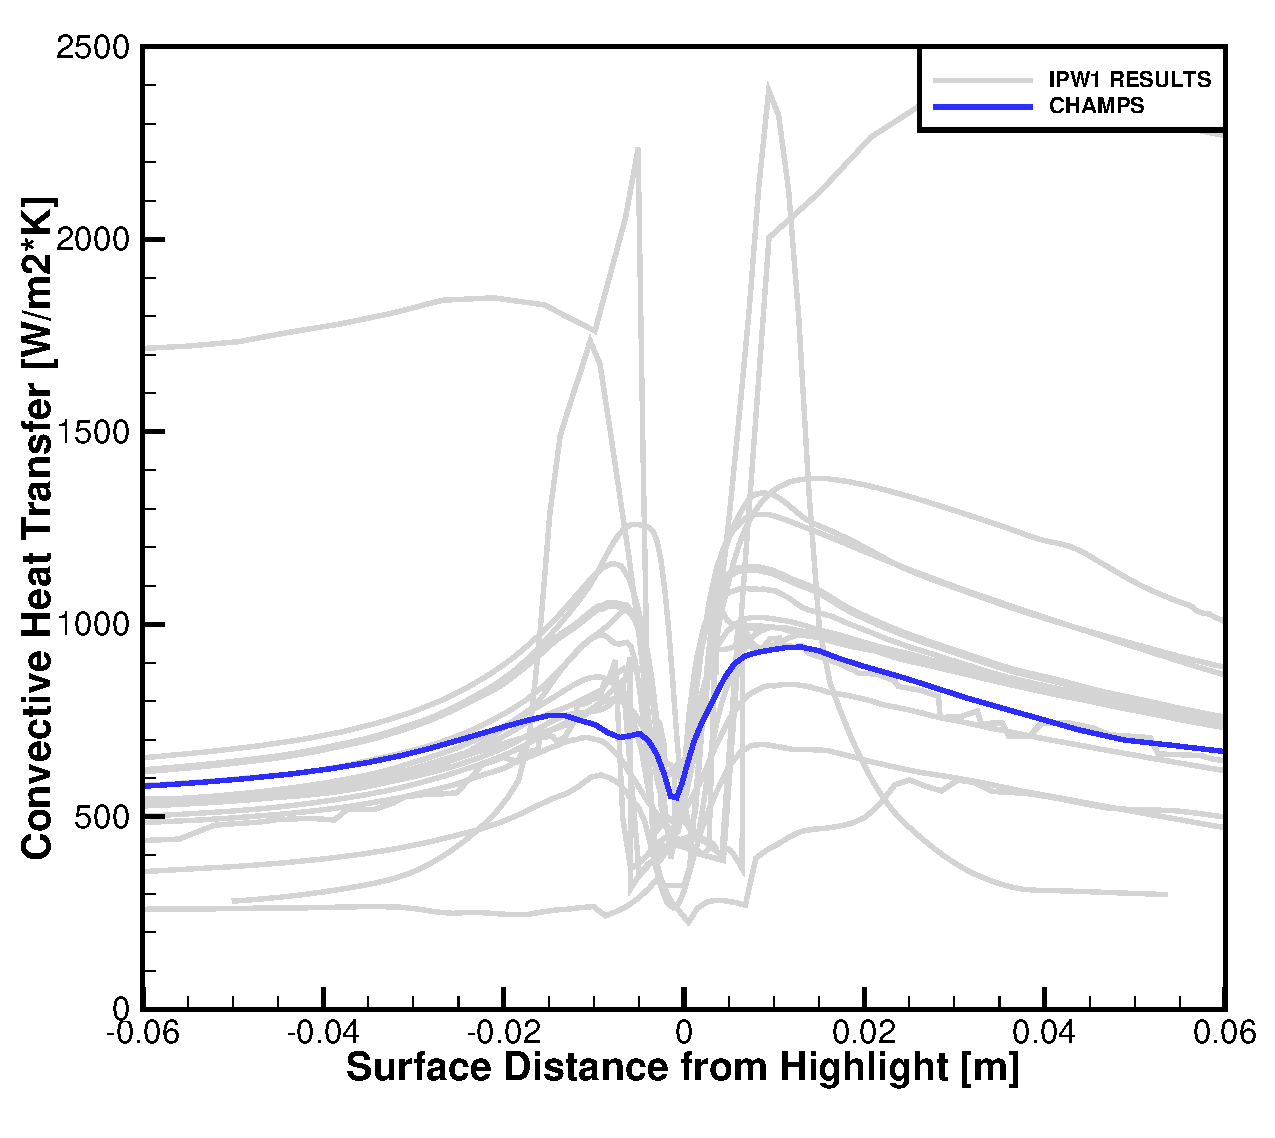
\includegraphics[trim={0cm 0cm 0cm 0cm},clip,width=0.32\textwidth]{FIGURES/LEVELSET_ARTICLE/CASE_IPW1_242_HTC.eps}
    \label{fig:Case242HTC}%
    }
    \caption{Comparison of the predicted aerodynamic and icing-related surface quantities for IPW1 Case 242 with the range of results submitted by IPW1 participants.}
    \label{fig:Case242VariablesResults}
\end{figure}

\begin{figure}[htbp] 
    \centering
    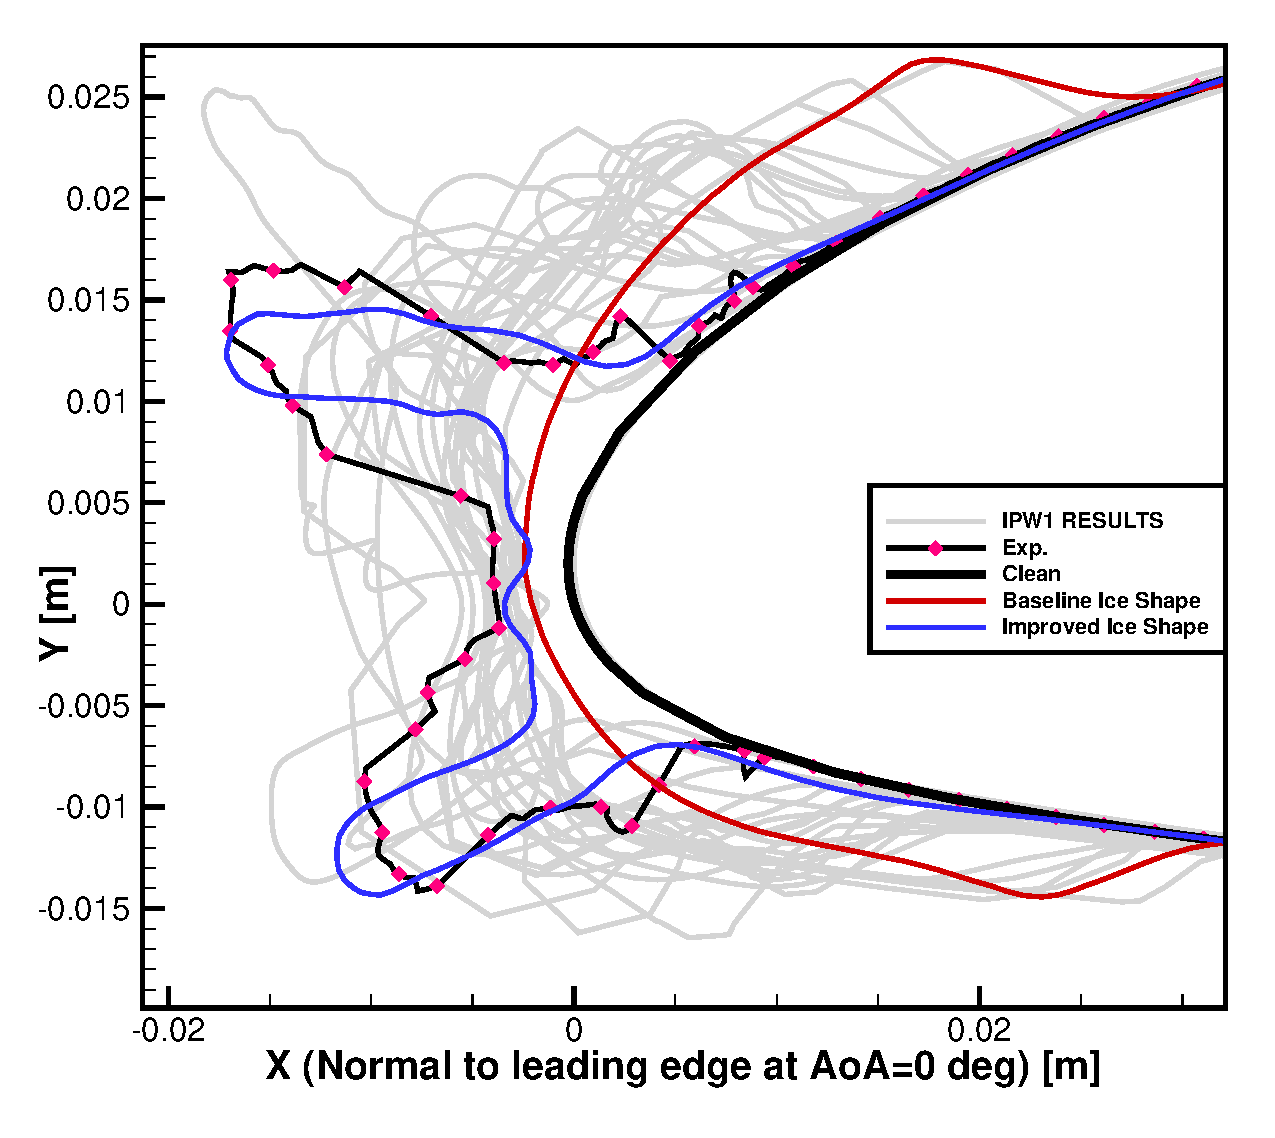
\includegraphics[trim={.1cm .1cm .1cm .1cm}, clip, width=0.5\textwidth]{FIGURES/LEVELSET_ARTICLE/CASE_IPW1_242_ICE_SHAPE.eps}
    \caption{Comparison of the predicted ice shapes for Case 242 obtained with different prescribed roughness values. Increasing \(k_s/c\) modifies the heat-transfer distribution and improves the predicted horn orientation.}
    \label{fig:iceShapeBaselineVsImproved}
\end{figure}

To assess whether the remaining discrepancy could be attributed to insufficient numerical convergence, a temporal convergence study was performed with respect to the number of accretion layers. The results showed that the predicted glaze ice shape reached convergence at approximately 20 layers, as illustrated in Figure~\ref{fig:Case242IceShapeLayerConvergence}. This indicates that the remaining differences with the experimental ice shape cannot be primarily attributed to the number of accretion layers and instead point to limitations associated with the physical modeling.

This finding suggests that another physical parameter plays a major role in glaze ice shape formation. Because the predicted HTC strongly influences the local freezing fraction and water runback, the parameters controlling convective heat transfer require further investigation. One of the key input parameters directly affecting HTC is the equivalent sand-grain roughness of the surface. Surface roughness enhances near-wall momentum exchange and promotes turbulence within the boundary layer, thereby increasing convective heat transfer at the wall. In the context of icing, a higher HTC promotes faster heat removal from the water film, thereby reducing liquid water runback and favoring earlier freezing closer to the impingement region. This mechanism is particularly important in glaze ice accretion, where the competition between water runback and local freezing largely governs horn development.

In the present simulations, no advanced roughness evolution model is yet available to update the roughness consistently from one accretion layer to the next. Consequently, the flow solver relies on a user-prescribed roughness value, which was initially set to $k_s/c = 0.001$ for the baseline solution, a value commonly adopted in the literature \cite{wright1997dra}. A second study was therefore performed to assess the influence of this parameter on horn formation. The results, presented in Figure~\ref{fig:Case242IceShapeKs}, show that increasing $k_s$ increases the HTC, which in turn reduces water runback and promotes earlier freezing as expected. This behavior strengthens horn formation and shifts the accretion toward shapes that are more representative of the experimental glaze ice geometry. In particular, larger roughness values lead to more pronounced horn development and reduce the downstream displacement of the horn tips. For the present case, among the values examined, \(k_s/c=0.003\) provides the best overall agreement with the experimental profile, especially in terms of horn angle, as highlighted in Table~\ref{tab:hornAngleComparison}. Some discrepancies nevertheless remain in horn thickness. This comparison suggests that roughness-driven HTC variations play a central role in glaze ice horn formation and should be modeled with greater physical fidelity. Future work will therefore investigate more elaborate roughness formulations.


\begin{figure}[htbp] 
    \subfloat[Layer convergence.]{%
    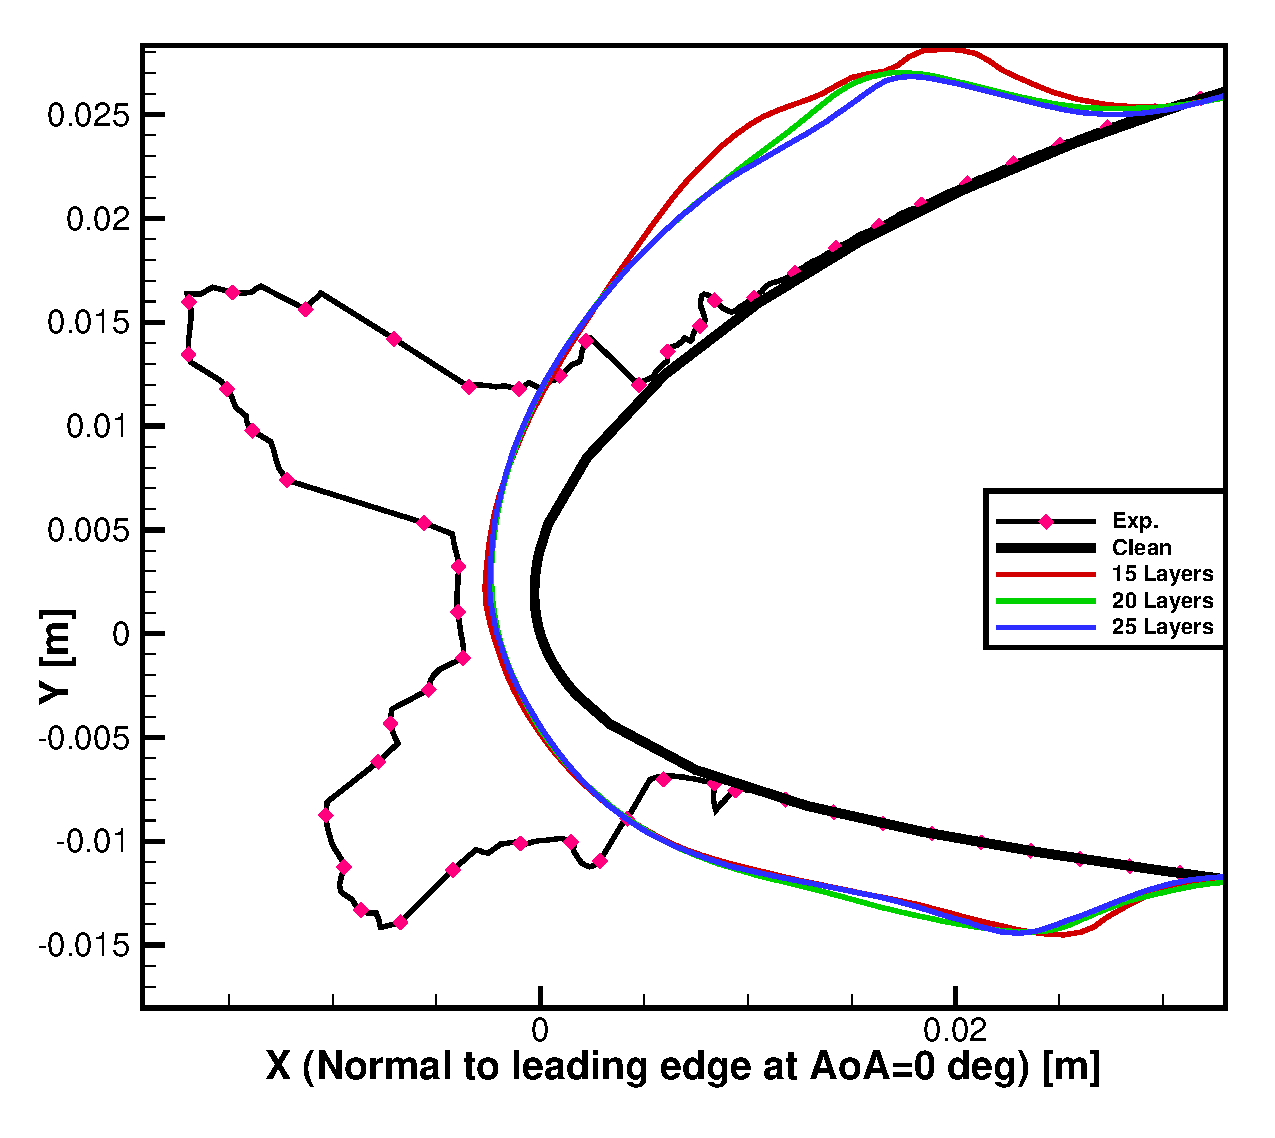
\includegraphics[trim={0cm 0cm 0cm 0cm},clip,width=0.325\textwidth]{FIGURES/LEVELSET_ARTICLE/Case242LayerConvergence.eps}
    \label{fig:Case242IceShapeLayerConvergence}%
    }
    \hspace*{0.1cm}
    \subfloat[HTC variation.]{%
    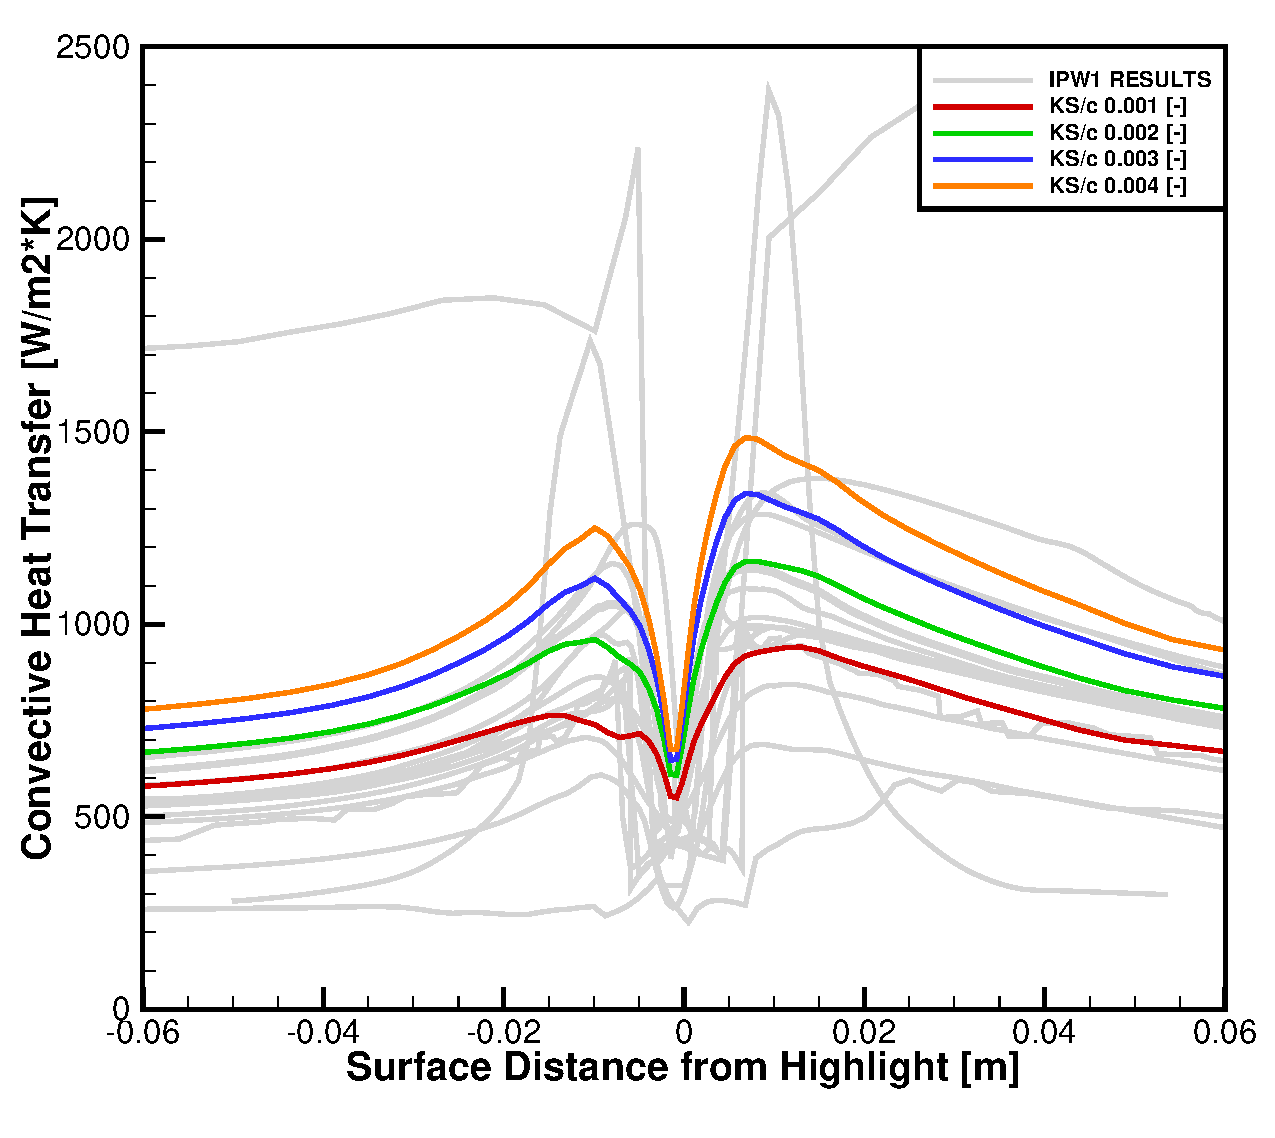
\includegraphics[trim={.1cm 0.1cm 0.1cm 0.1cm},clip,width=0.325\textwidth]{FIGURES/LEVELSET_ARTICLE/Case242HTCVariation.eps}
    \label{fig:Case242IceShapeHighlights}%
    }
    \subfloat[Ice shape variation.]{%
    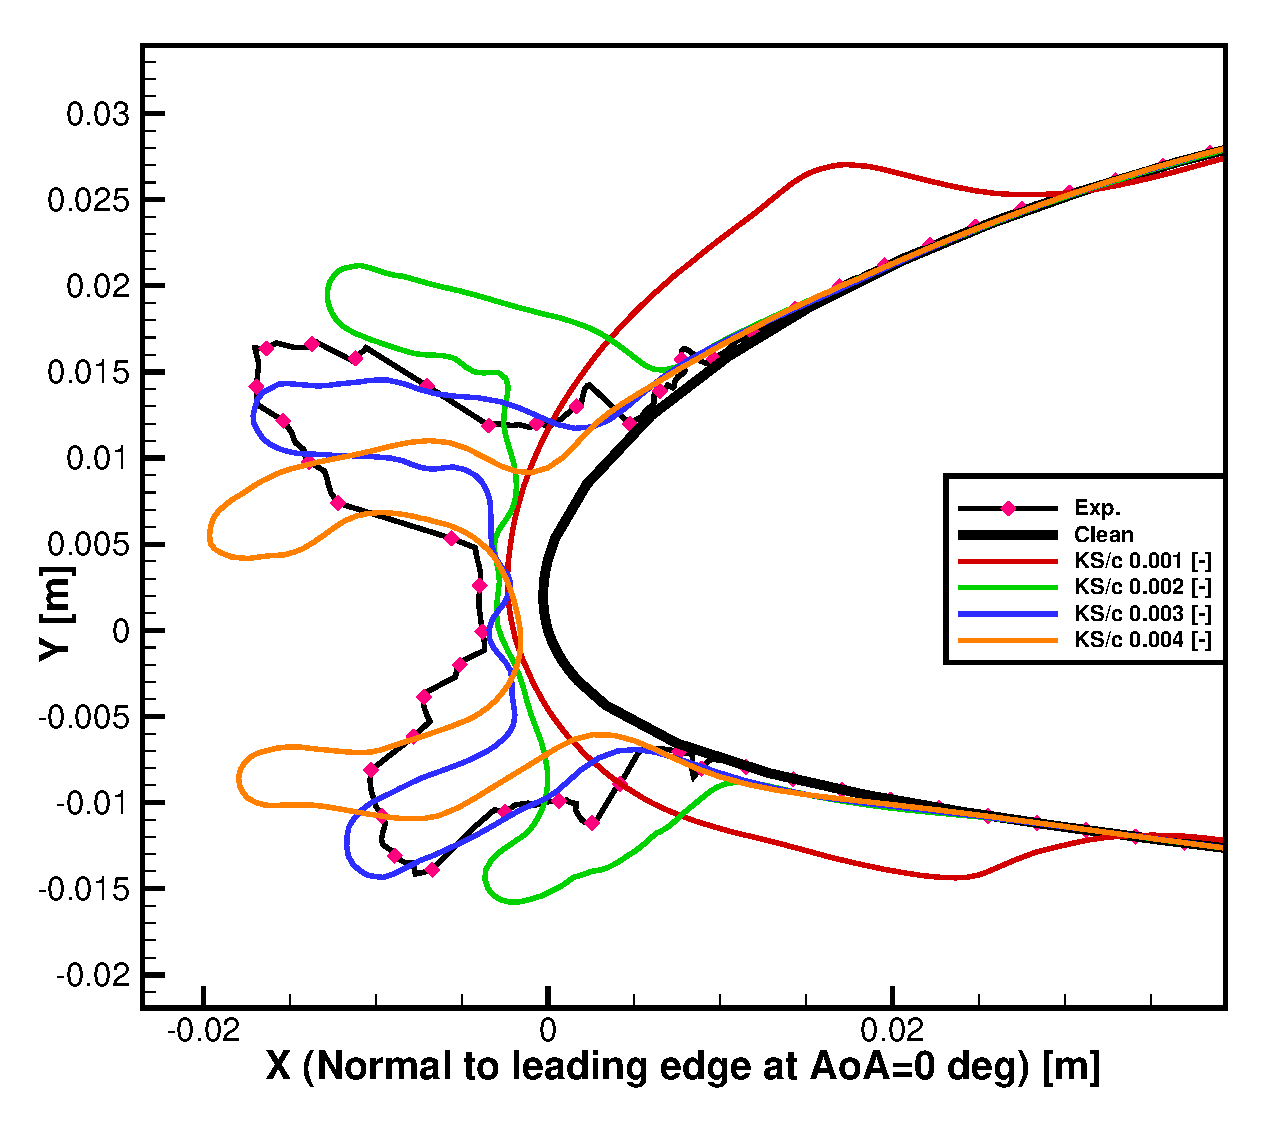
\includegraphics[trim={0cm 0cm 0cm 0cm},clip,width=0.325\textwidth]{FIGURES/LEVELSET_ARTICLE/Case242RoughnessVariation.eps}
    \label{fig:Case242IceShapeKs}%
    }

    \caption{Comparison of glaze ice predictions for Case 242: temporal convergence with respect to the number of accretion layers, variation of the heat transfer coefficient (HTC) with roughness magnitude $k_s$, and influence of $k_s$ on the predicted ice shape.}
    \label{fig:Case242Ice}
\end{figure}

In contrast to the previous case, for which the overall accretion remains relatively compact and the maximum ice height provides a meaningful scalar indicator, the characterization of the present glaze ice case is more appropriately based on the orientation of the upper and lower horns. For this reason, the horn angles were selected as the primary quantitative metrics for this case. The smallest roughness value, $k_s/c = 0.001$, is not considered in the analysis, as no clear horn formation is observed for this configuration.

The horn angles were computed using reference points extracted from the experimental ice shape (Fig.~\ref{fig:hornAnglesMeasurement}). Specifically, for each horn, upper and lower, a representative point was identified at the midpoint of the corresponding horn region. The associated reference point on the clean airfoil was then defined as the closest point on the clean geometry to this experimental horn location. These experimentally derived reference points were subsequently used consistently for all roughness cases.

\begin{figure}[htbp] 
    \centering
    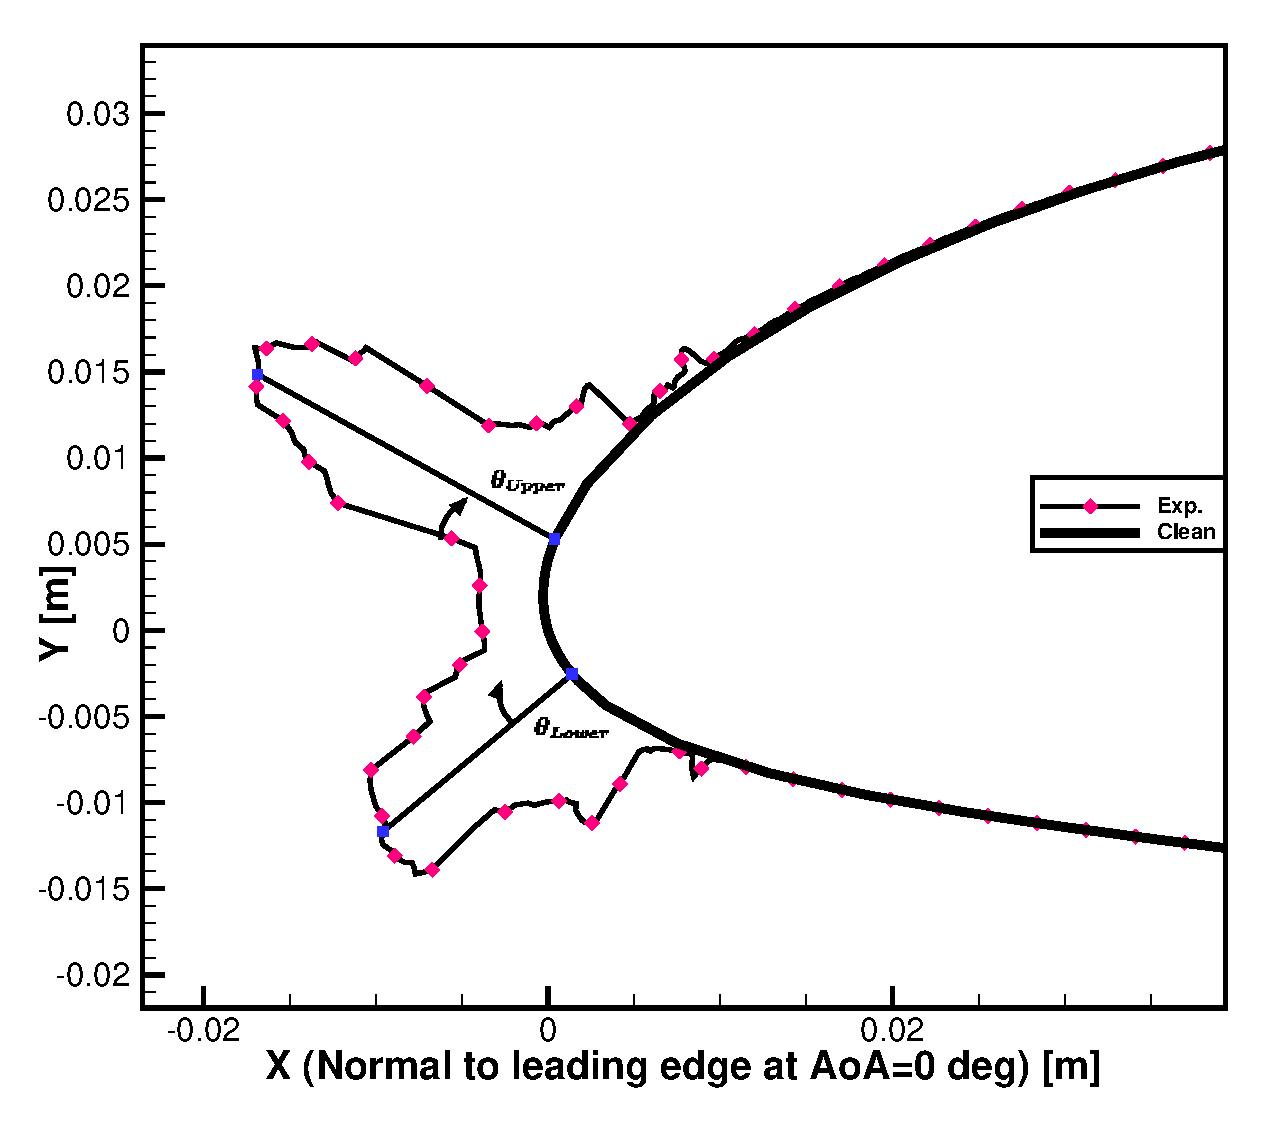
\includegraphics[trim={.1cm .1cm .1cm .1cm}, clip, width=0.5\textwidth]{FIGURES/LEVELSET_ARTICLE/Case242HornAngles.eps}
    \caption{Definition of the horn angles on the experimental ice shape.}
    \label{fig:hornAnglesMeasurement}
\end{figure}

For a given roughness case $k_s$, the horn tip was identified as the point exhibiting the largest upstream extension, that is, the most negative $x$-coordinate. The horn angle was then computed as the angle between the vector connecting the clean reference point to the selected horn tip and the horizontal axis passing through.

The comparison reported in Table~\ref{tab:hornAngleComparison} shows that the predicted horn orientation is strongly affected by the prescribed roughness level. Among the values considered, the case $k_s/c=0.003$ yields the best overall agreement with the experimental reference, with relative errors of $22.9\%$ and $5.96\%$ for the upper and lower horn angles, respectively. Lower roughness values underpredict the horn deviation and lead to angles that remain too close to the airfoil surface, whereas the largest roughness value does not further improve the agreement. Instead, it appears to over-promote local freezing and modifies the horn morphology such that the measured horn angles are again underpredicted.

\begin{table}[ht]
\centering
\caption{Comparison of the upper and lower horn angles for Case 242, together with the relative error with respect to the experimental reference.}
\begin{tabular}{cccccc}
\hline \hline
Config. & $k_s/c \, [-]$ & $\theta_{Upper}$ [$^\circ$] & Upper rel. error [\%] & $\theta_{Lower}$ [$^\circ$] & Lower rel. error [\%] \\
\hline
Exp. & --    & $29.00$ & --    & $39.77$ & --    \\
2    & $0.002$ & $46.69$ & $60.96$ & $66.89$ & $68.21$ \\
3    & $0.003$ & $22.34$ & $22.99$ & $37.39$ & $5.96$  \\
4    & $0.004$ & $0.63$  & $97.83$ & $17.34$ & $56.39$ \\
\hline \hline
\end{tabular}
\label{tab:hornAngleComparison}
\end{table}

\subsection{Case IPW1 361}
\label{subsec:3D_case_361}

Case 361 involves a $30^\circ$ swept NACA 0012 wing configuration tested in a wind tunnel. According to the workshop conditions, this case corresponds to a rime ice regime. Figure~\ref{fig:Case361VariablesResults} presents the obtained predictions for the aerodynamic and icing-related surface quantities. Overall, a good agreement is observed with the envelope of the IPW1 participants' results, indicating that the main physical trends are well captured by the present framework.

\begin{figure}[ht!]
\hspace*{0cm}
    \subfloat[Pressure coefficient.]{%
    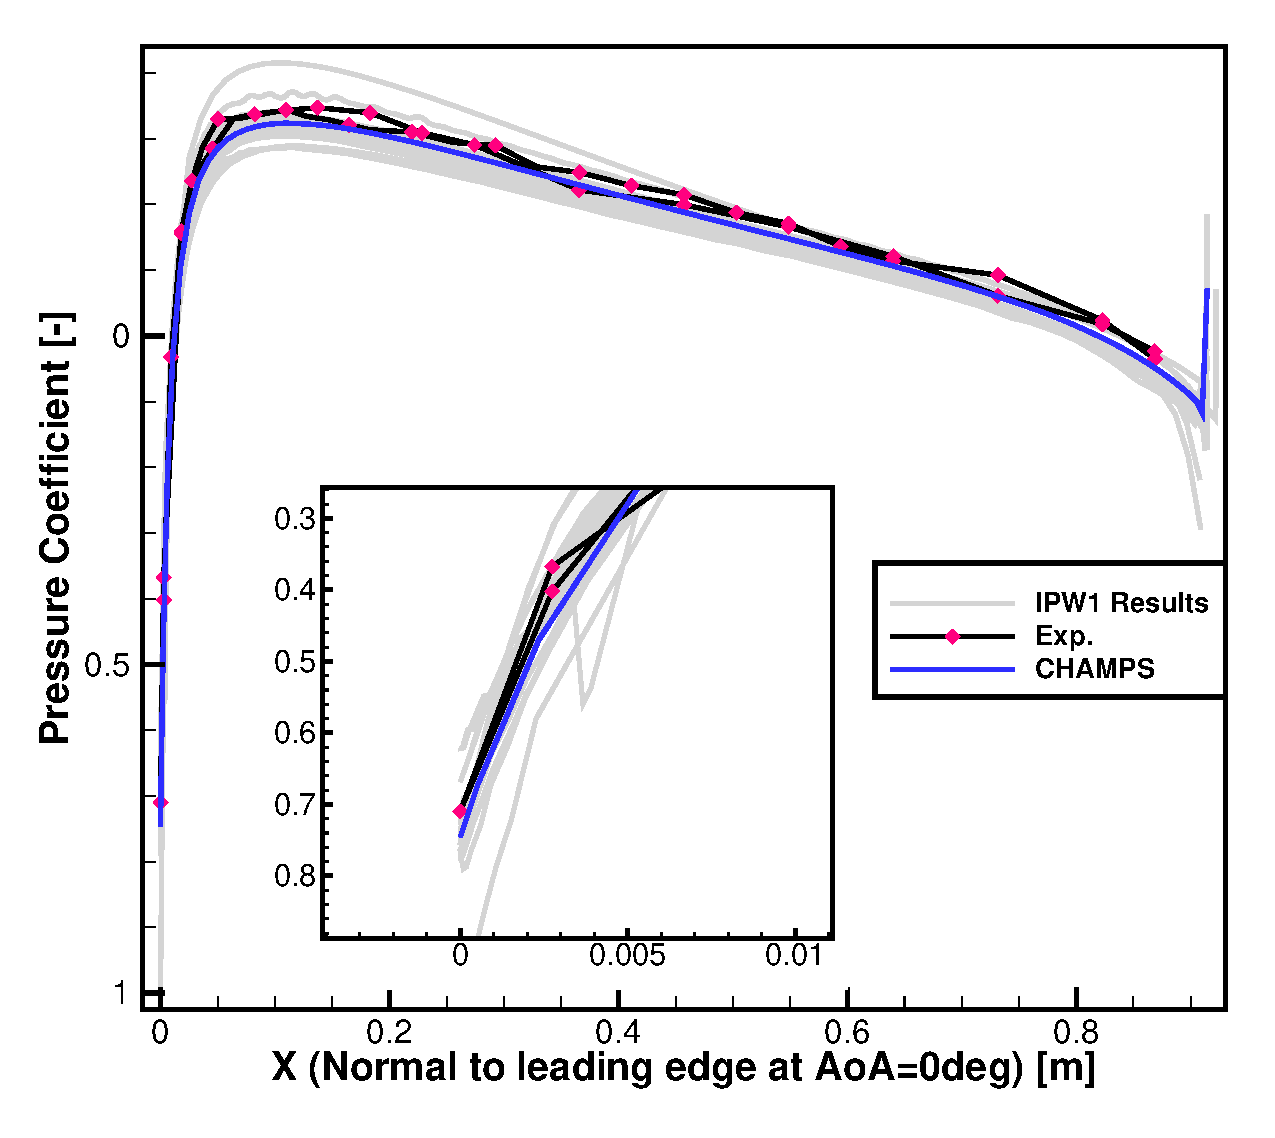
\includegraphics[trim={0cm 0cm 0cm 0cm},clip,width=0.32\textwidth]{FIGURES/LEVELSET_ARTICLE/CASE_IPW1_361_CP.eps}
    \label{fig:Case361Cp}%
    }
    \hspace*{0.1cm}
    \subfloat[Collection efficiency.]{%
    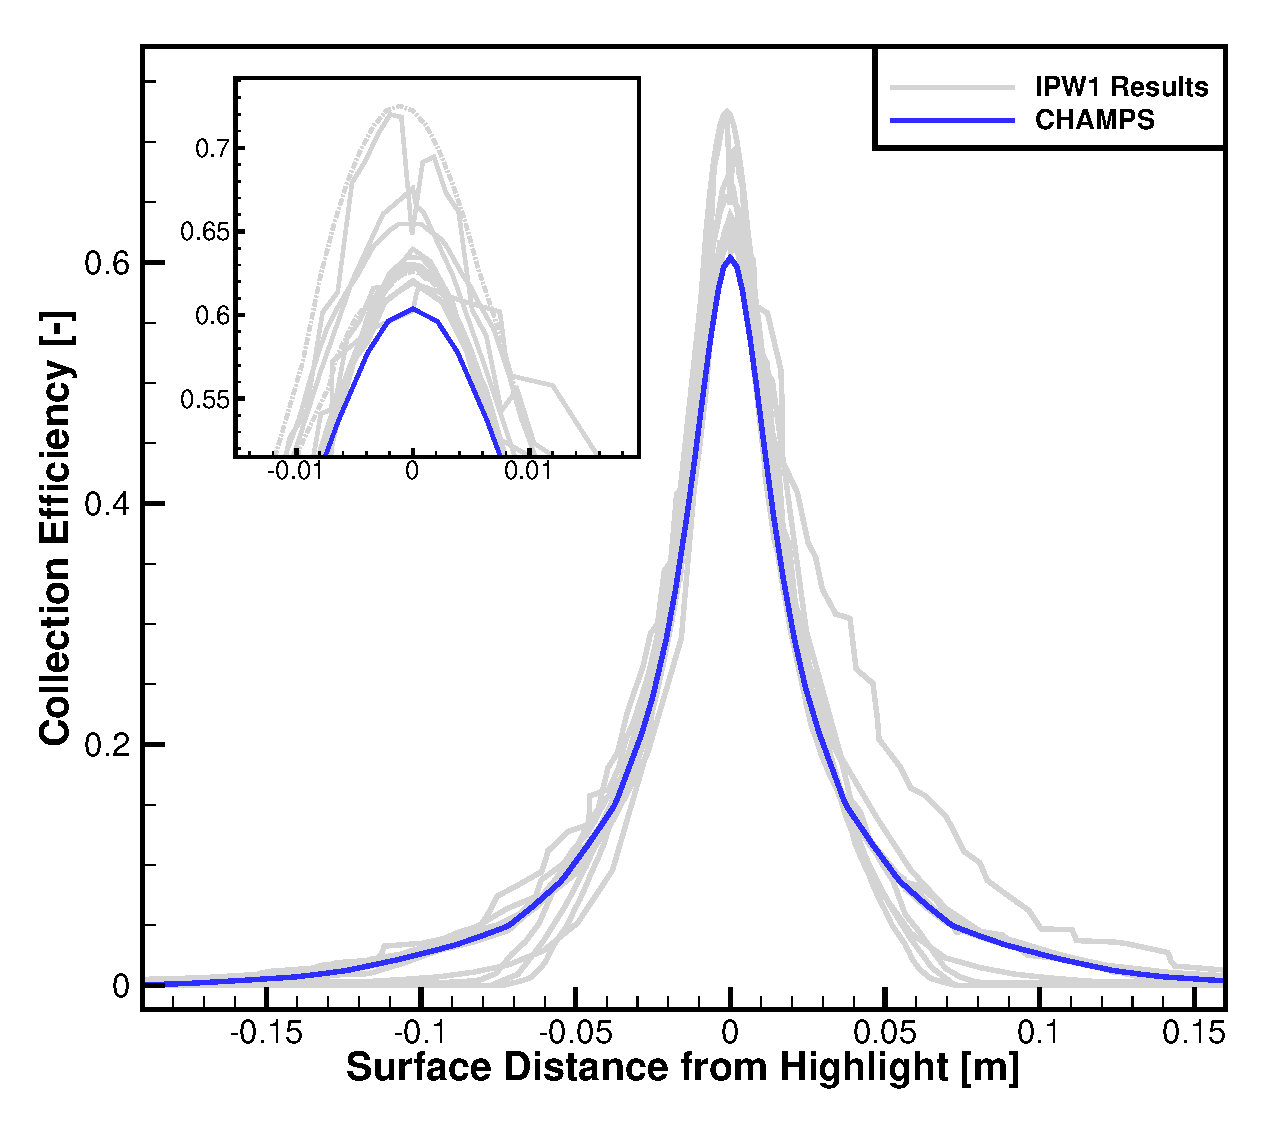
\includegraphics[trim={0cm 0cm 0cm 0cm},clip,width=0.32\textwidth]{FIGURES/LEVELSET_ARTICLE/CASE_IPW1_361_BETA.eps}
    \label{fig:Case361Beta}%
    }
    \hspace*{0.1cm}
    \subfloat[Convective heat transfer.]{%
    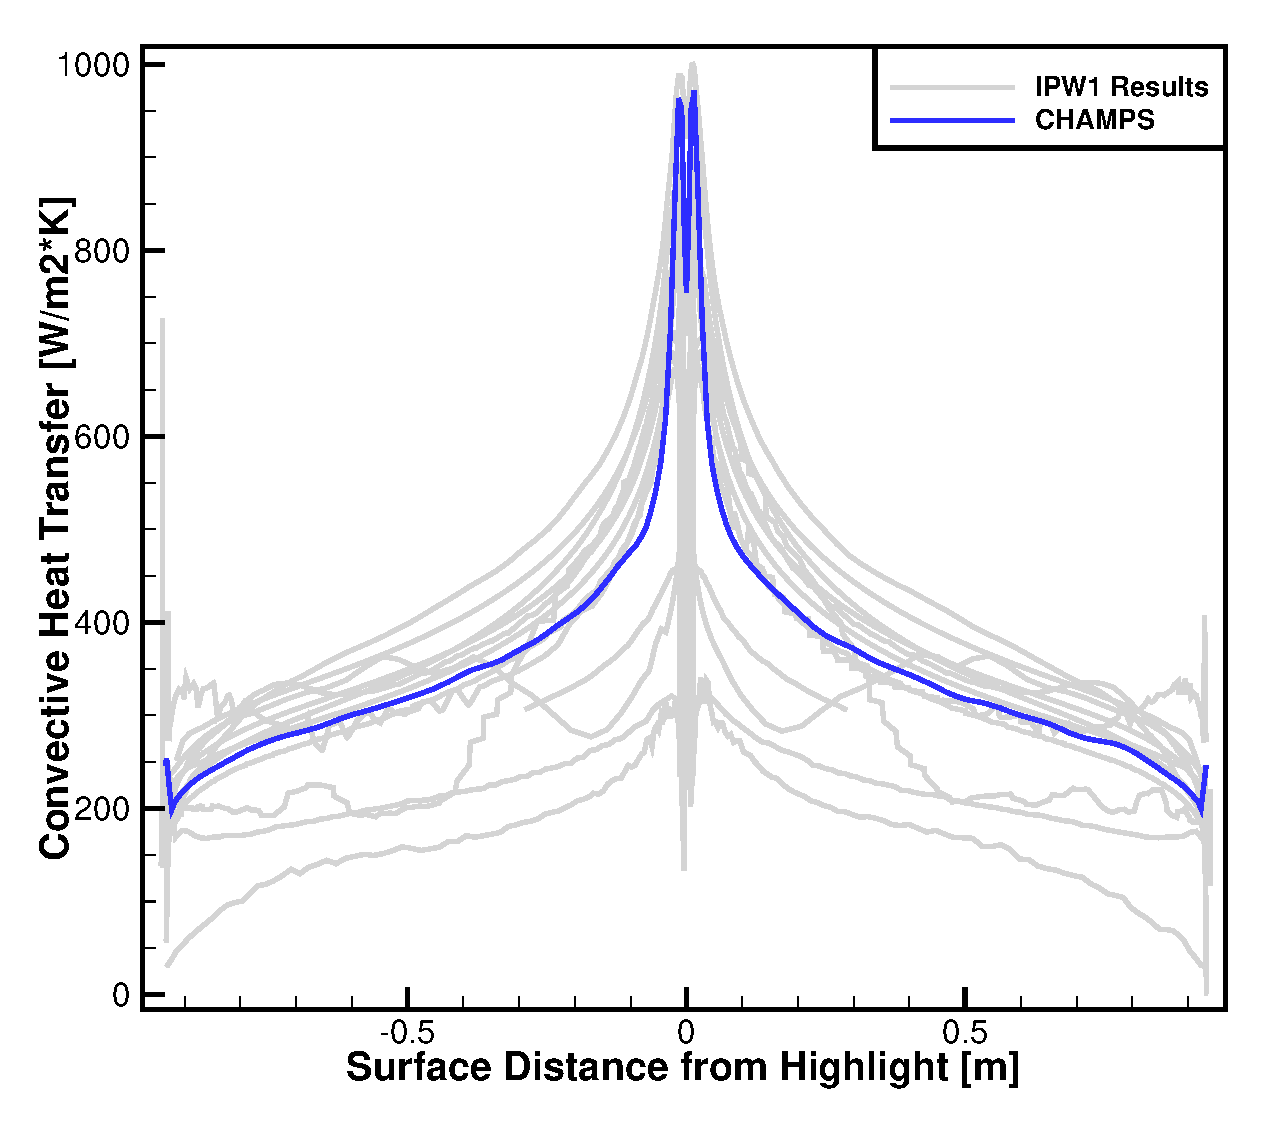
\includegraphics[trim={0cm 0cm 0cm 0cm},clip,width=0.32\textwidth]{FIGURES/LEVELSET_ARTICLE/CASE_IPW1_361_HTC.eps}
    \label{fig:Case361HTC}%
    }
    \caption{Comparison of the predicted aerodynamic and icing-related surface quantities for IPW1 Case 361 against the results submitted by IPW1 participants.}
    \label{fig:Case361VariablesResults}
\end{figure}

Figure~\ref{fig:Case361Ice} compares the ice shapes obtained with 1, 2, and 5 accretion layers against the experimental ice shape and the IPW1 participants' results. The predicted shapes were post-processed following the workshop guidelines by extracting maximum combined cross sections (MCCS) from the computed 3D ice shape. In contrast with the behavior observed for the previous cases, the single-layer prediction appears to remain the closest to the experimental ice shape. A similar trend was also reported by \cite{alessandroLevelSet}. As the number of layers increases, the predicted ice shape becomes progressively thicker and more streamlined, which is consistent with the behavior expected for a rime ice case.

This tendency suggests that the discrepancy may not primarily originate from the numerical treatment of the geometric update, but rather from the experimental accretion conditions themselves. More specifically, the flatter and less protruding experimental ice shape may indicate that the accretion did not correspond to an ideal purely rime regime, or that additional physical effects not included in the present model influenced the final geometry.

\begin{figure}[ht!] 
    \subfloat[Comparison of predicted ice shapes by the level-set]{%
    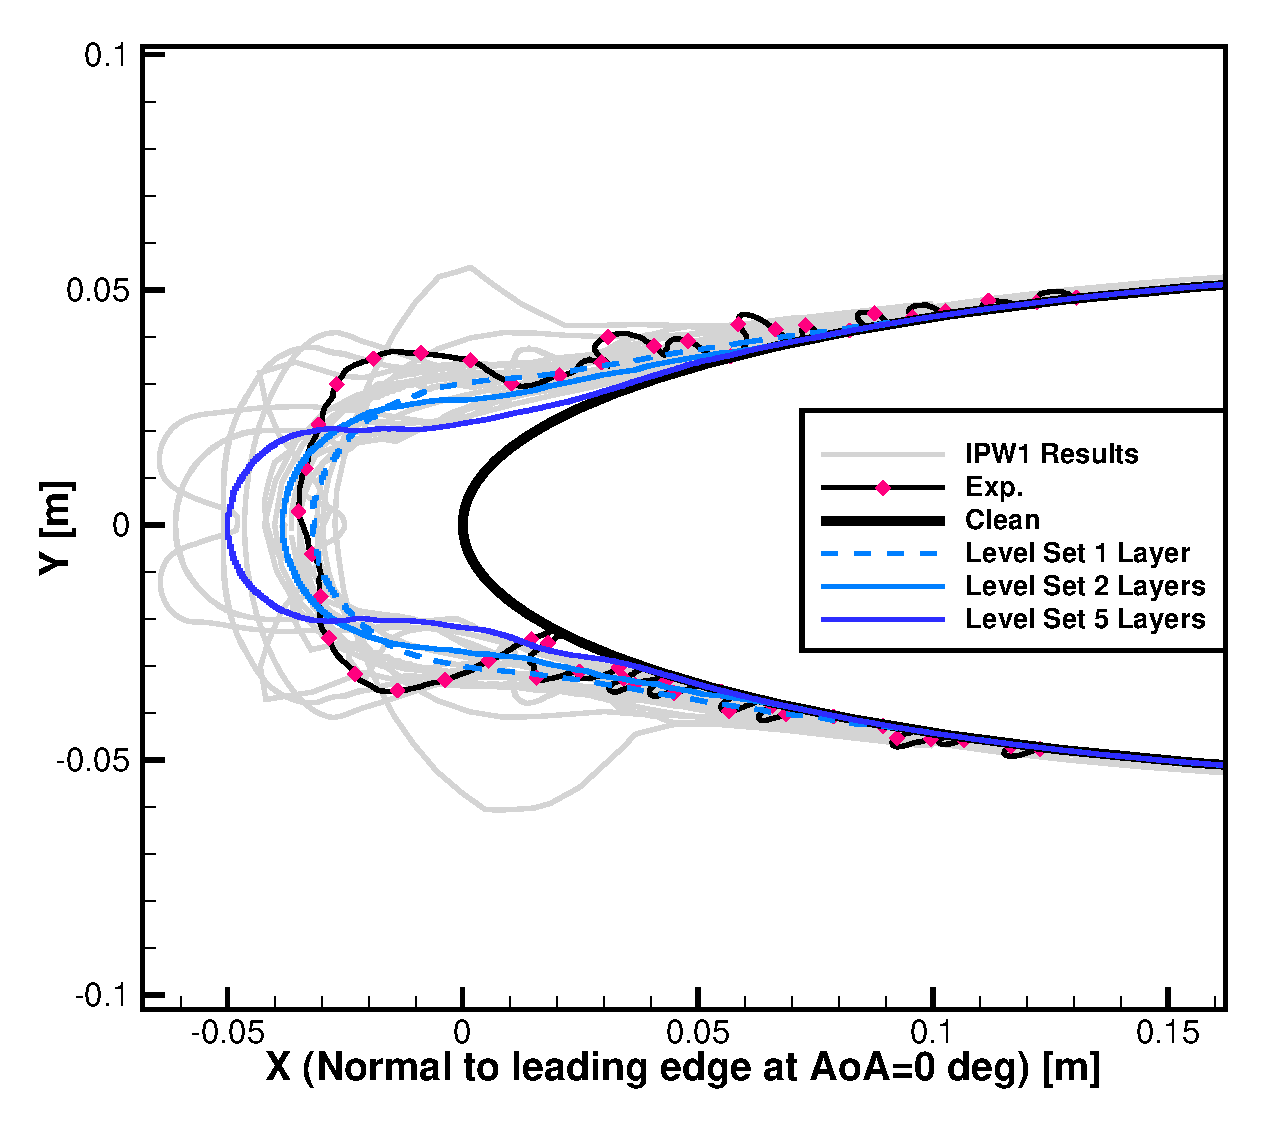
\includegraphics[trim={0cm 0cm 0cm 0cm},clip,width=0.5\textwidth]{FIGURES/LEVELSET_ARTICLE/CASE_IPW1_361_ICE_SHAPE.eps}
    \label{fig:Case361IceShape}%
    }
    \subfloat[Clipped view of the 5-layer ice shape]{%
    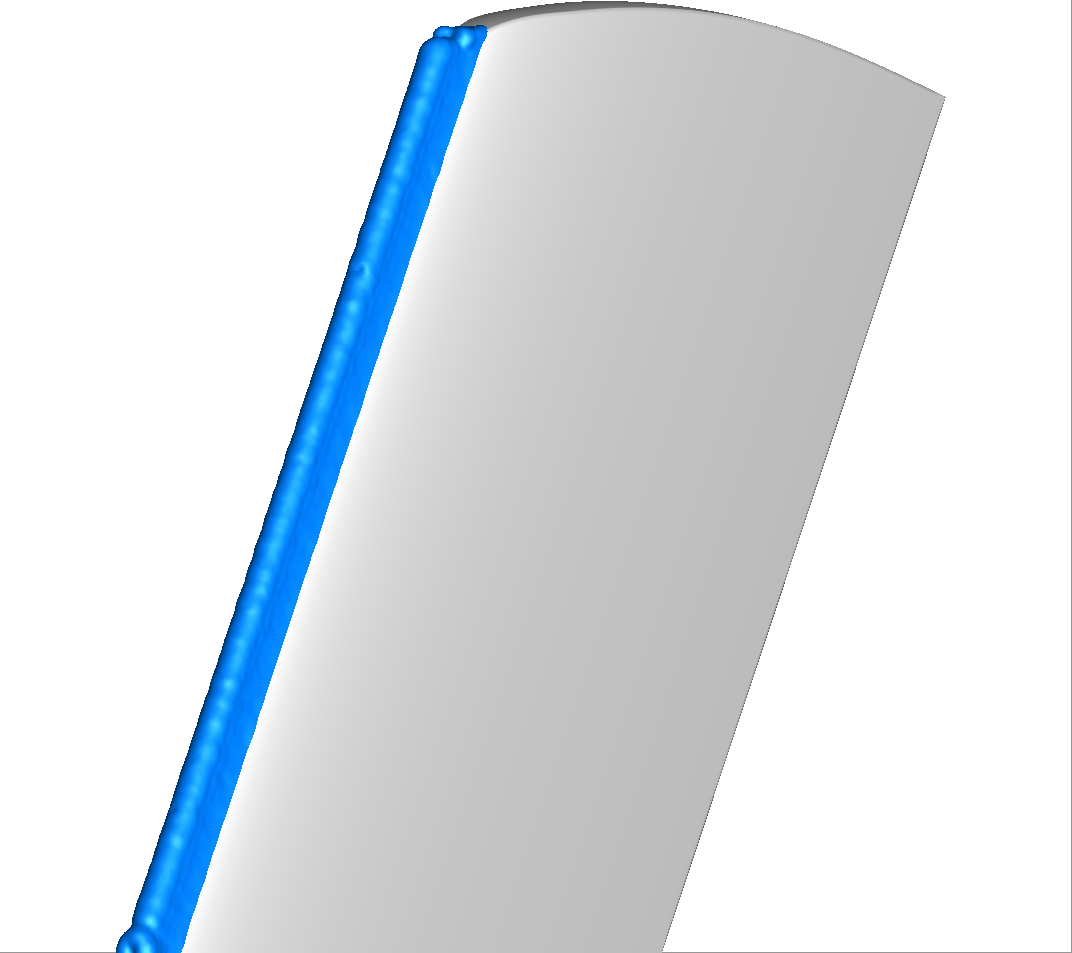
\includegraphics[trim={1cm 0.1cm 1cm 0.1cm},clip,width=0.5\textwidth]{FIGURES/LEVELSET_ARTICLE/CLIPPED_ICE_SHAPE_CASE_361.png}
    \label{fig:Case361ClippedIceShape}%
    }
    \caption{Predicted ice shapes for Case 361. The effect of the number of accretion layers on the final ice shape is shown for 1, 2, and 5 layers, together with the experimental ice shape and the IPW1 participants' results. A 3D view of the predicted accreted geometry is also presented.}
    \label{fig:Case361Ice}
\end{figure}

\subsection{Case IPW1 362}
\label{subsec:3D_case_362}
Following the previous rime ice case, Case 362 is characterized by similar aerodynamic and icing conditions, with the main difference being the higher static temperature. Although this change has only a limited effect on the aerodynamic flow field, it plays a central role in the resulting ice morphology. As discussed previously, increasing the temperature reduces the local freezing fraction and promotes liquid water runback along the surface. The water can then freeze farther downstream, leading to more complex glaze ice shapes. In the present swept wing configuration, this behavior is associated with the formation of spanwise scallop structures with non-uniform size and spacing. Such features are consistent with the 3D nature of glaze ice accretion on swept wings, where the spanwise flow component, liquid-water runback, and local heat-transfer variations can promote non-uniform ice growth. These features are illustrated in Fig.~\ref{fig:Case362Clip}.

\begin{figure}[ht!]
\hspace*{0cm}
    \subfloat[Clipped view of the 10-layer ice shape]{%
    %\fbox{%
    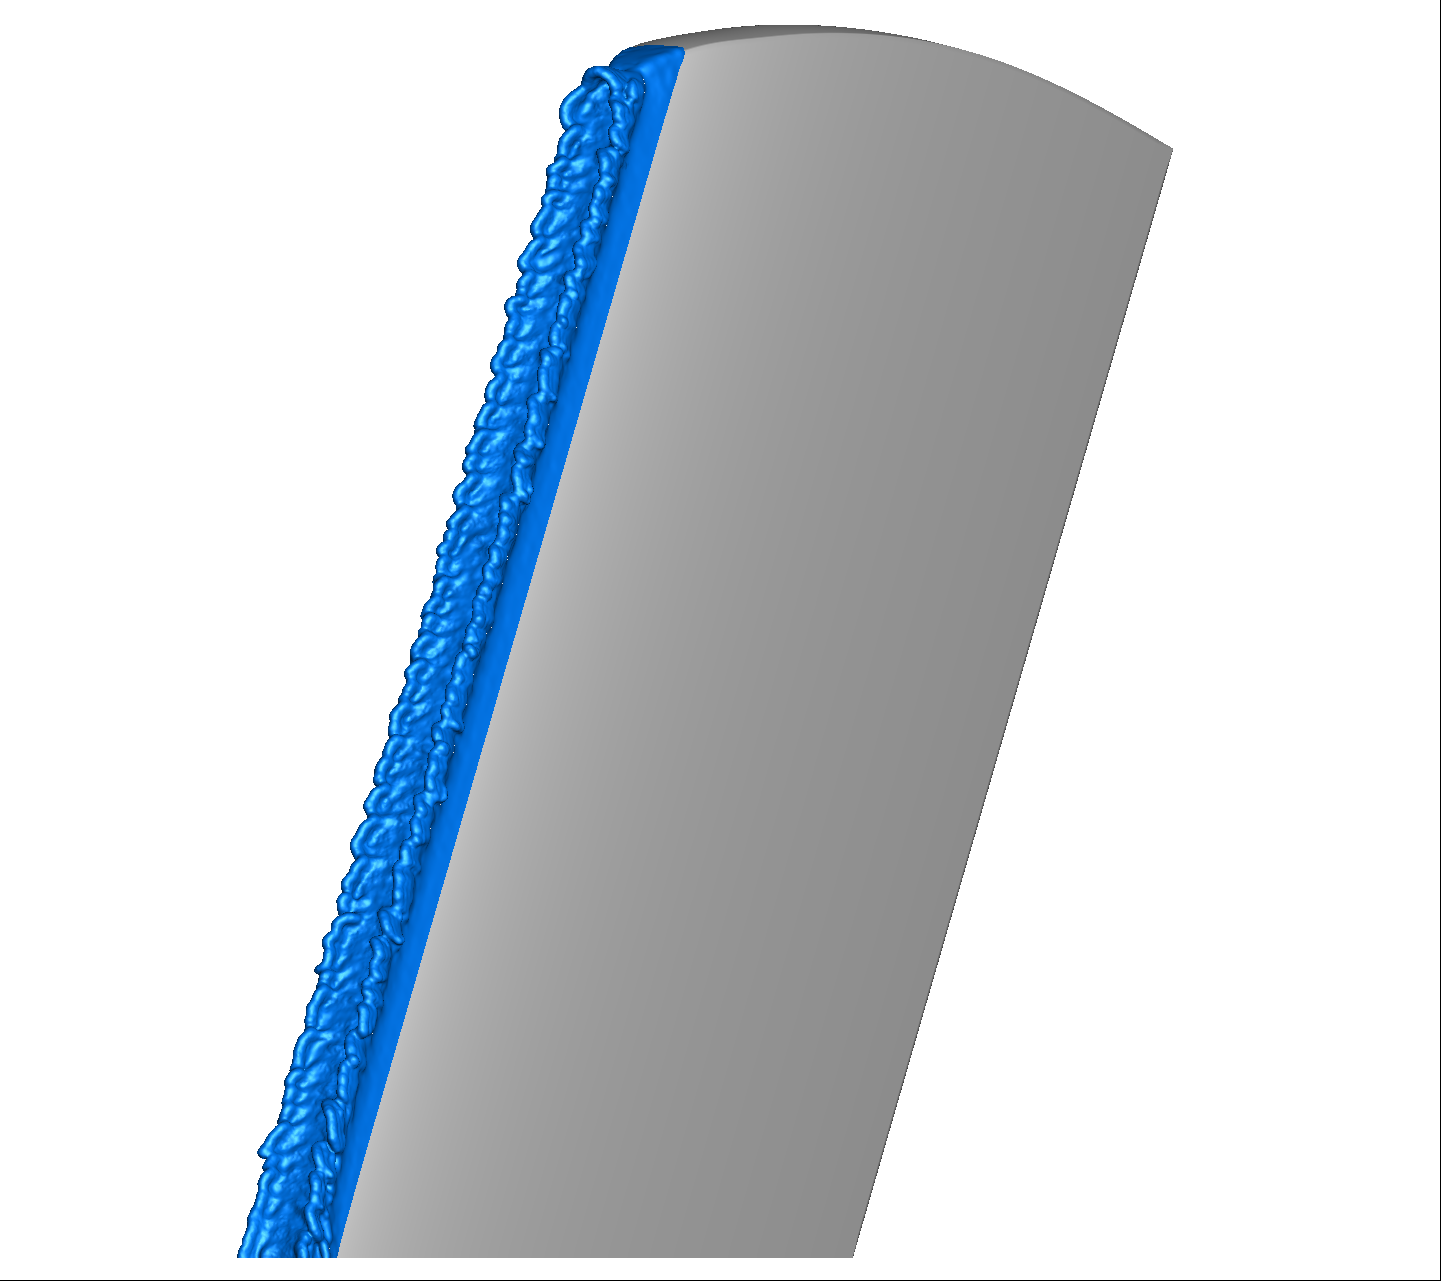
\includegraphics[trim={8cm 1cm 9.5cm 1cm},clip,width=0.305\textwidth]
    {FIGURES/LEVELSET_ARTICLE/CLIPPED_ICE_SHAPE_CASE_362_1.png}
    %}
    \label{fig:Case362Clip1}%
    }
    \hspace*{0.1cm}
    \subfloat[Spanwise scallop structures]{%
    %\fbox{%
    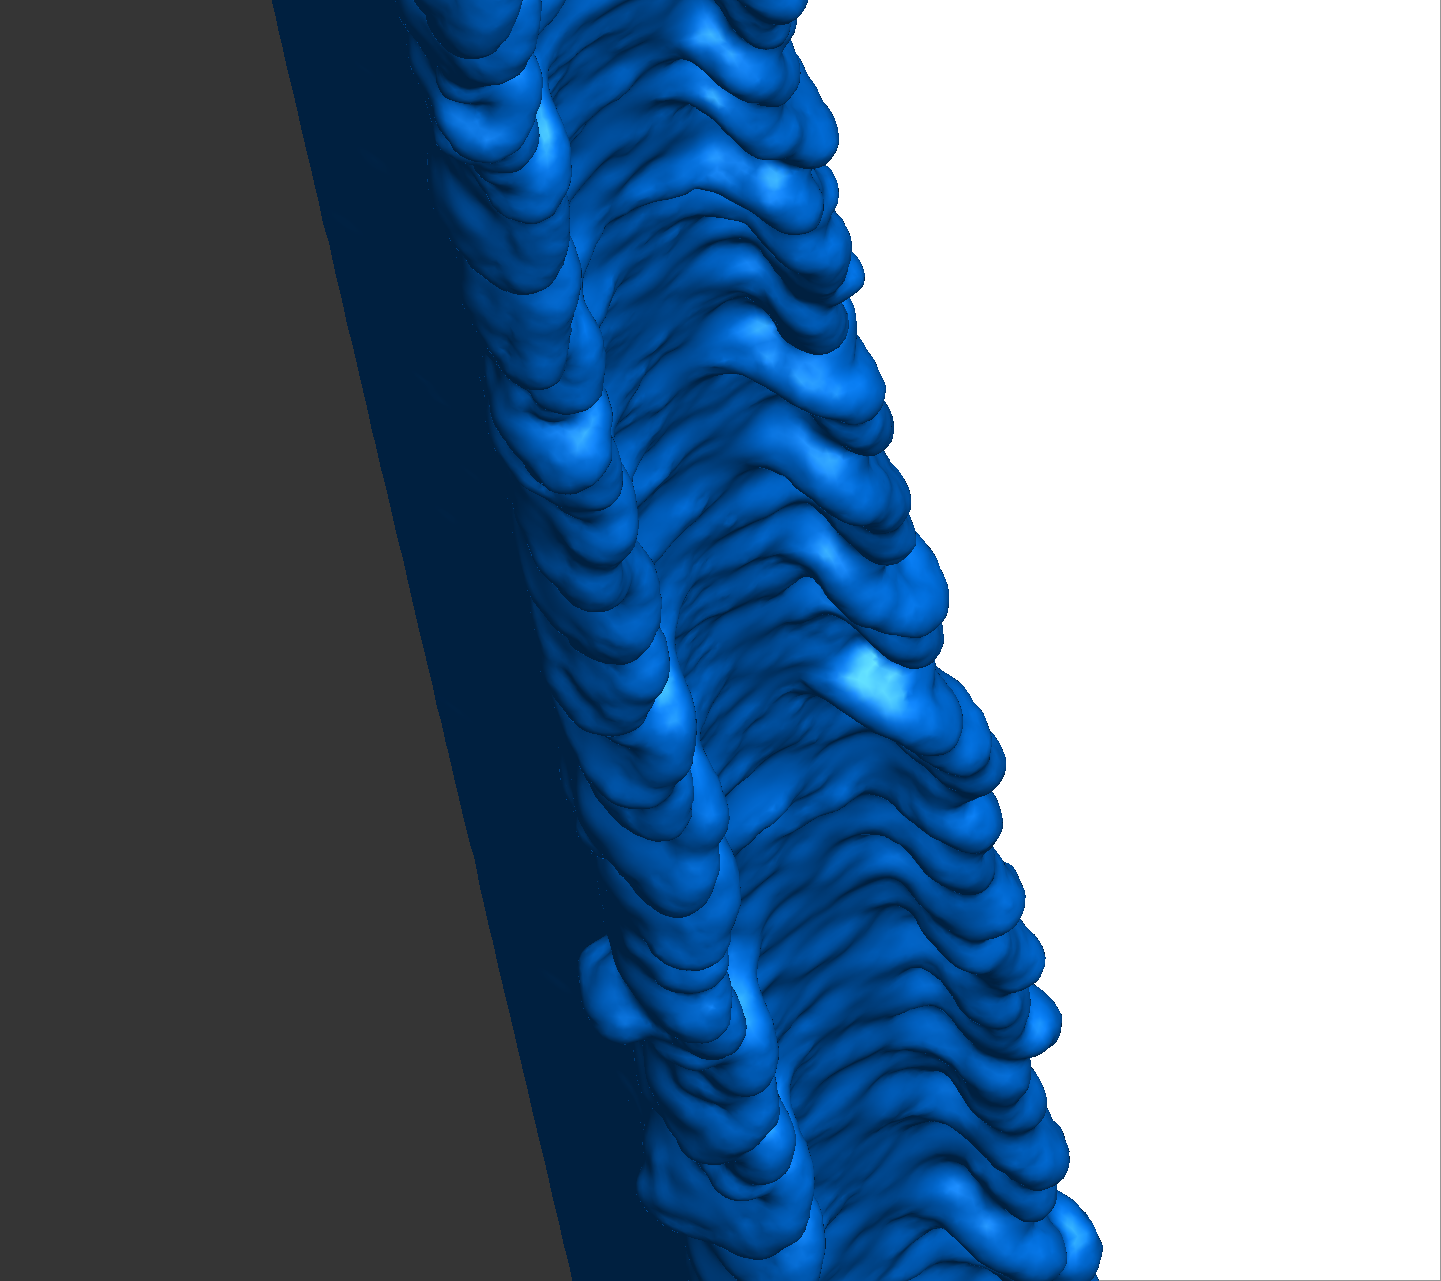
\includegraphics[trim={1cm 0.1cm 12cm 0.1cm},clip,width=0.305\textwidth]{FIGURES/LEVELSET_ARTICLE/CLIPPED_ICE_SHAPE_CASE_362_2.png}
    %}
    \label{fig:Case362Clip2}%
    }
    \hspace*{0.1cm}
    \subfloat[Adapted surface mesh on the ice shape]{%
    %\fbox{%
    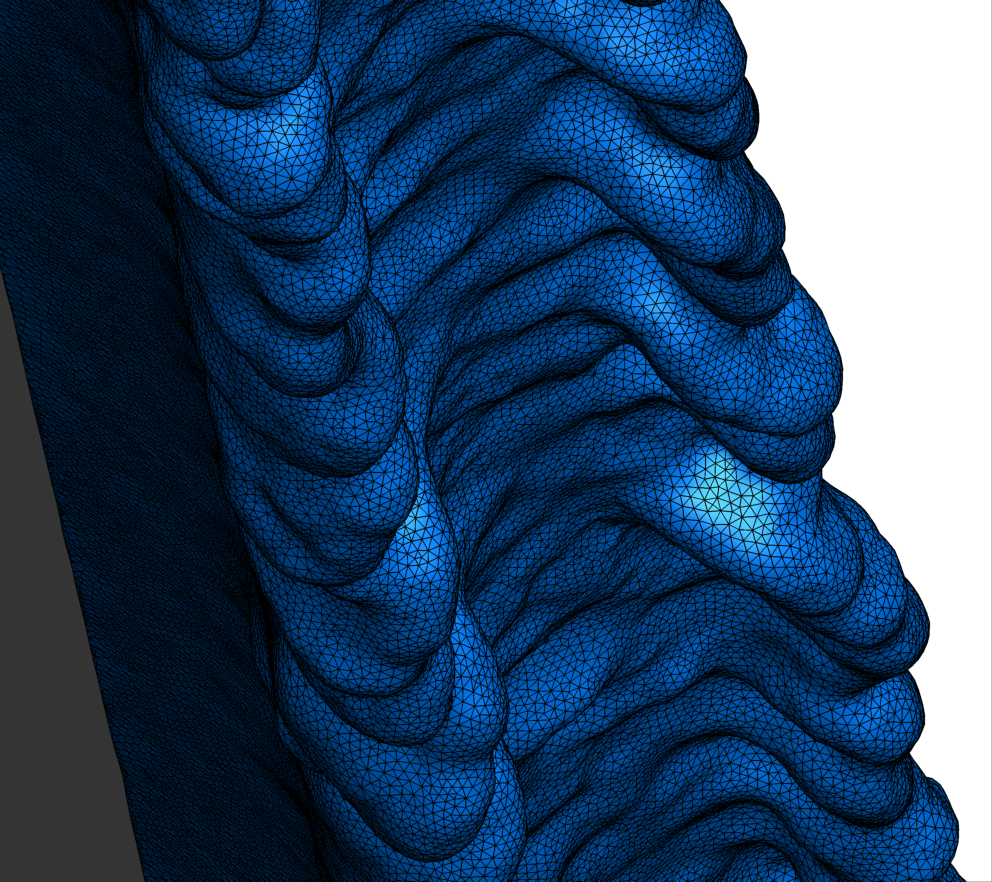
\includegraphics[trim={1cm 0.1cm 2cm 0.1cm},clip,width=0.38\textwidth]{FIGURES/LEVELSET_ARTICLE/CLIPPED_ICE_SHAPE_CASE_362_3.png}
    %}
    \label{fig:Case362Clip3}%
    }
    \caption{Predicted 3D ice shape for IPW1 Case 362 after 10 accretion layers. The clipped views illustrate the spanwise scallop structures formed along the leading edge and the corresponding adapted surface mesh after level-set extraction.}
    \label{fig:Case362Clip}
\end{figure}

In contrast with the rime ice case, a multilayer approach is essential for this glaze ice configuration in order to progressively capture the development of the complex scallop structures, as shown in Fig.~\ref{fig:IceShapeCase362}. The MCCS obtained with 10 accretion layers shows reasonably good overall agreement with the experimental ice shape. However, discrepancies remain near the impingement limits and in the predicted horn orientation. The simulation was performed using a constant roughness height of $k_s/c=0.001$. As shown in the previous cases, the prescribed roughness is an important parameter controlling the horn orientation and downstream water runback. In the present 3D case, the surface features generated under this imposed roughness may have locally limited the runback process, which could partly explain the mismatch observed near the impingement limits.

Figure~\ref{fig:IceShapeCase362_MCCS_VS_SLICE} presents a comparison of the predicted ice shape using a local spanwise slice extracted at the midspan location and the corresponding MCCS representation. Since the experimental data are only available in the form of an MCCS, a direct comparison with the local experimental morphology is not possible. However, the predicted results clearly illustrate how the MCCS can smooth and damp local spanwise variations, masking important 3D features of the ice accretion. This emphasizes the limitations of assessing highly 3D ice shapes using only 2D cross-sectional representations, since they may not fully capture the local morphology of the accretion. Future work should therefore aim to develop improved 3D comparison tools and more representative quantitative metrics for evaluating the agreement between predicted and experimental ice shapes.

\begin{figure}[ht!]
\hspace*{0cm}
    \subfloat[Effect of the number of accretion layers]{%
    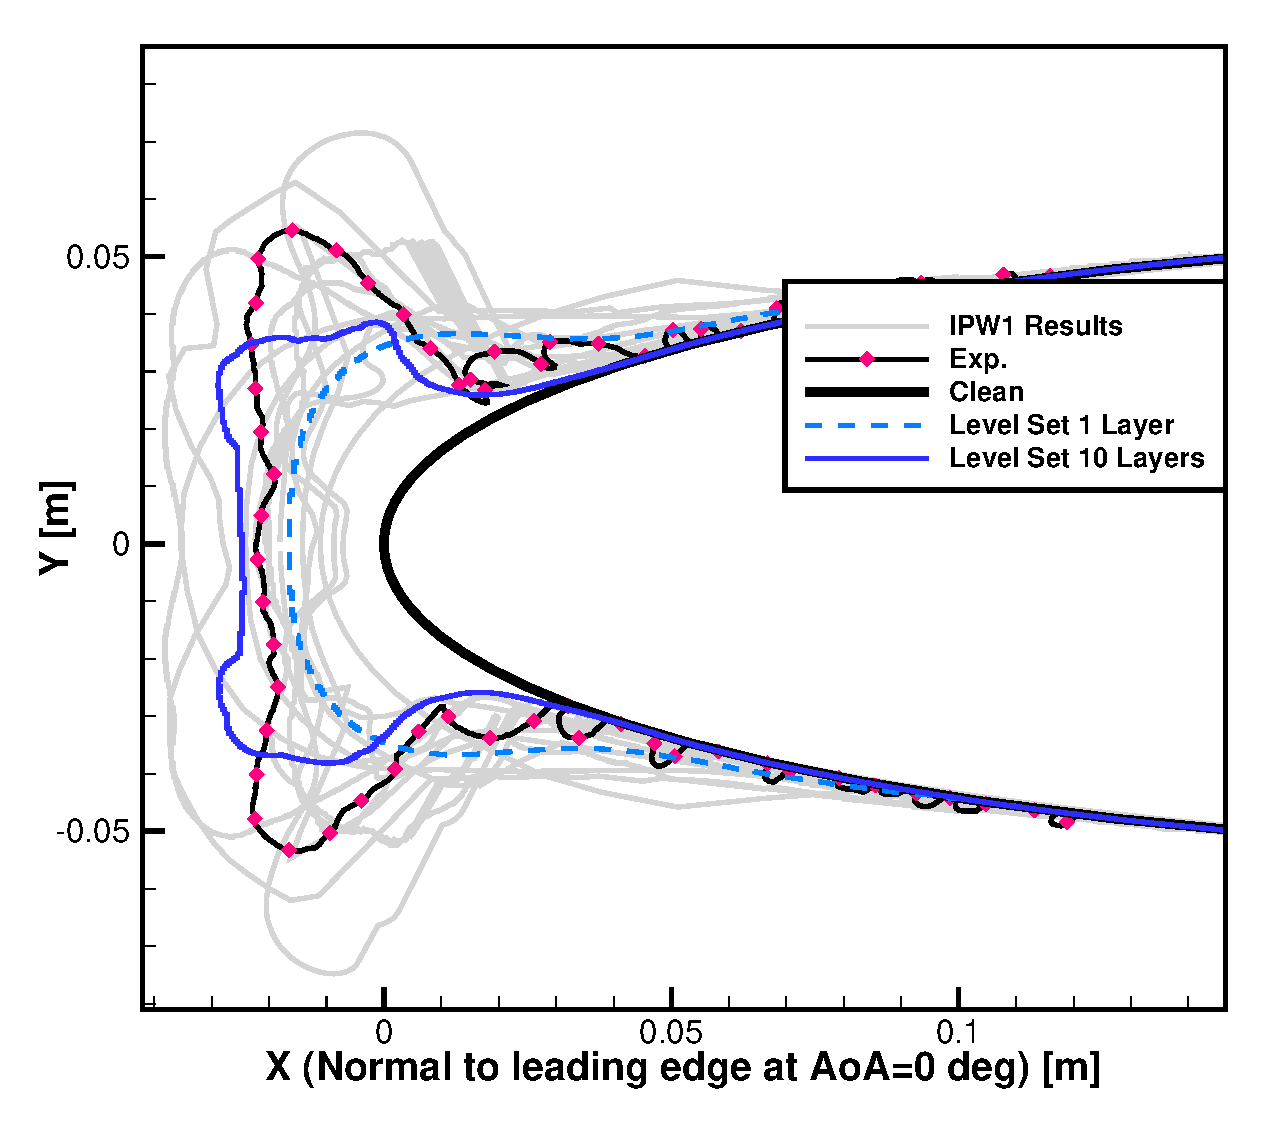
\includegraphics[trim={0cm 0cm 0cm 0cm},clip,width=0.5\textwidth]{FIGURES/LEVELSET_ARTICLE/CASE_IPW1_362_ICE_SHAPE.eps}
    \label{fig:IceShapeCase362}%
    }
    \hspace*{0.1cm}
    \subfloat[Comparison between midspan slice and MCCS extraction]{%
    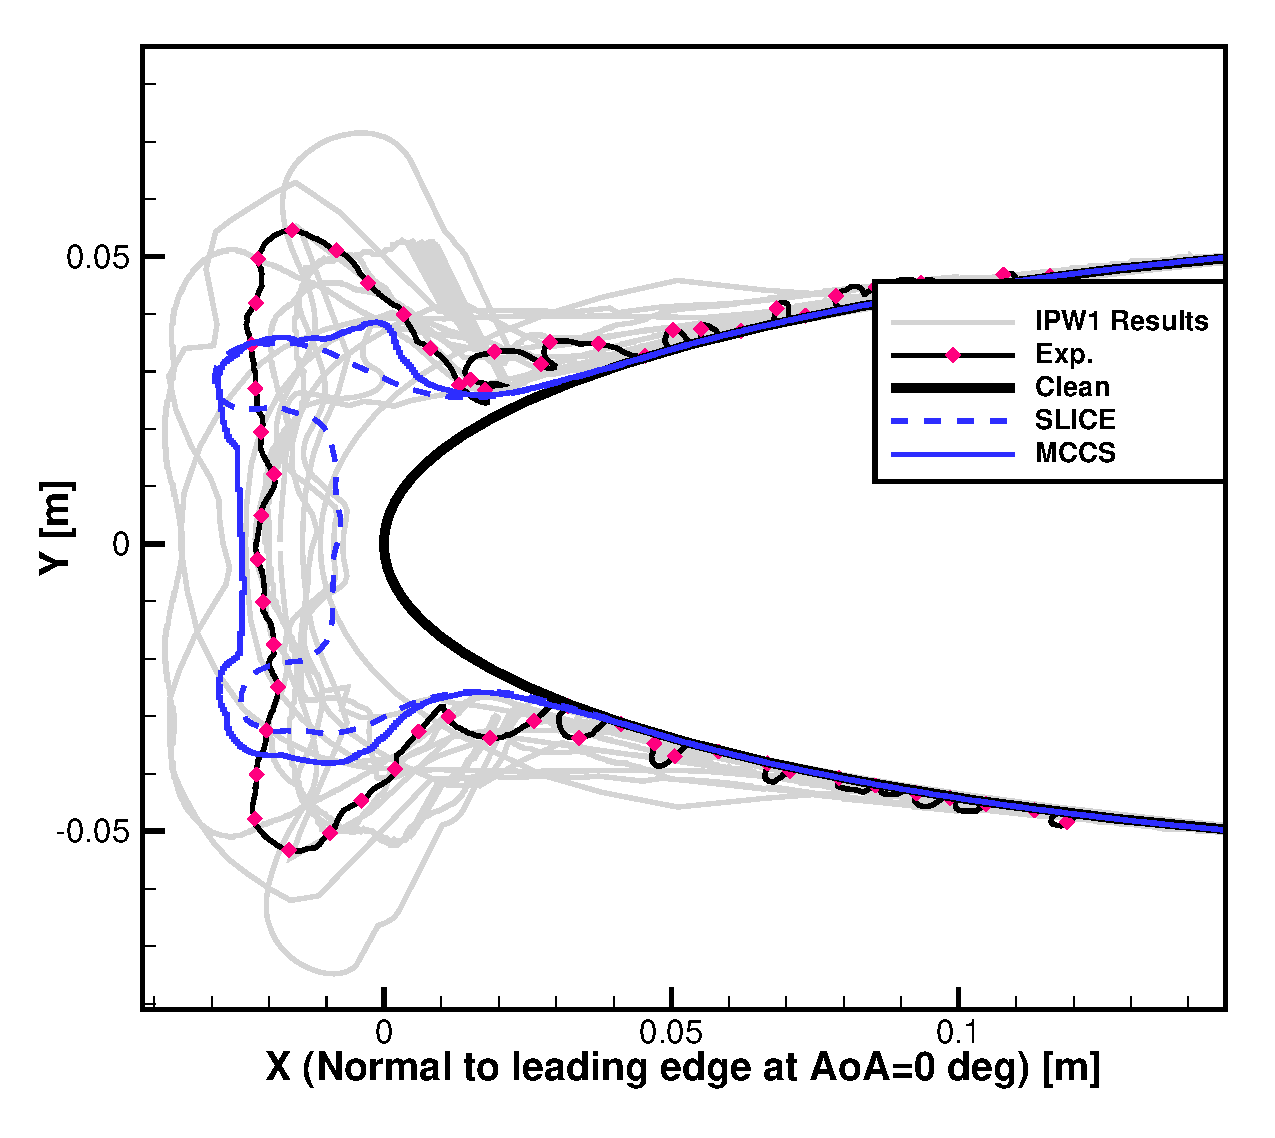
\includegraphics[trim={0cm 0cm 0cm 0cm},clip,width=0.5\textwidth]{FIGURES/LEVELSET_ARTICLE/CASE_IPW1_362_ICE_SHAPE_MCCS_vs_SLICE.eps}
    \label{fig:IceShapeCase362_MCCS_VS_SLICE}%
    }
    \caption{Predicted ice shapes for IPW1 Case 362. The experimental ice shape, clean airfoil profile, and IPW1 participant results are shown for reference. The level-set predictions obtained with 1 and 10 accretion layers are compared, together with the ice shape extracted from a single spanwise slice and the maximum combined cross-section (MCCS) extracted from the 3D ice shape.}
    \label{fig:IceShapeCase362Comp}
\end{figure}

\section{Conclusion}
\label{sec:conclusionsLS}

This work presented a level-set based framework for 3D multilayer ice accretion simulations within the \textsc{CHAMPS} solver. The proposed methodology combines a conservative level-set formulation, a semi-implicit Rosenbrock--Wanner time integration strategy, local interface reconstruction for ice-volume evaluation, and zero level set extraction using \textsc{MMG} to generate conformal surface geometries. In addition, a smoothing procedure was introduced to regularize the extracted interface while preserving the overall geometric integrity of the accreted ice shape. Altogether, these elements provide a robust alternative to traditional Lagrangian node-displacement methods, particularly for configurations involving complex geometric features and possible topological changes.

The proposed framework was assessed on both manufactured and experimental benchmark cases. The results showed that the method is capable of capturing complex ice-shape evolutions while maintaining good agreement with reference solutions and experimental data. In particular, the level-set formulation demonstrated clear advantages in terms of geometric robustness and conformity of the extracted interface. The analysis of the glaze ice case also highlighted the strong sensitivity of horn formation to the convective heat-transfer and, consequently, to the prescribed surface roughness.

Future work will focus on improving the physical modeling of glaze ice accretion. In particular, more advanced local roughness models will be investigated to represent the spatial and temporal evolution of surface roughness throughout successive accretion layers, rather than relying on a prescribed uniform equivalent sand-grain roughness. Such developments are expected to improve the prediction of local heat transfer, water runback, and ultimately glaze ice horn formation. In addition, future efforts should also address the comparison of highly 3D ice shapes with experimental measurements by developing improved comparison tools and quantitative metrics that better preserve local morphological features.
